%---------------------------------------------------------------------------------------------------
% Note: Use pdflatex to process this file.
%---------------------------------------------------------------------------------------------------

\documentclass[10pt]{book}

%%\usepackage[all]{nowidow}
\usepackage{index}
\usepackage{setspace}
\usepackage{graphicx}
\usepackage{moreverb}    % Defines {listing} environment.
\usepackage{amsmath, amsthm, amssymb, amsbsy, mathtools}
\usepackage{alltt}
\usepackage{rotating}
\usepackage{subcaption}
\usepackage{xspace}
\usepackage{xcolor}
%%\usepackage{makeidx}
\usepackage[section]{placeins}   % For preventing floats from floating to end of chapter.
\usepackage{longtable}  % For splitting long vertical tables into pieces
\usepackage{multirow}
\usepackage{booktabs}   % For table layouts
\usepackage{yhmath}     % For widehat
\usepackage{eso-pic}    % For cover graphics
\usepackage{enumitem}
%%\usepackage{fancyvrb}
\usepackage{biblatex}
\usepackage[T1]{fontenc}   % so _, <, and > print correctly in text.
\usepackage[strings]{underscore}    % to use "_" in text
\usepackage[pdftex,colorlinks=true,bookmarksnumbered=true]{hyperref}   % Must be last package!

\addbibresource{bibliography.bib}   % compile with `biber AcceleratorLattice`

%---------------------------------------------------------------------------------------------------
% Etienne stuff

\newcommand{\RR}{\textrm{I\kern-0.19emR}}
\newcommand{\CC}{\textrm{I\kern-0.5emC}}
\newcommand{\dragt}{\mbox{\scriptsize $\begin{matrix}\# \\
\# \end{matrix}$}}
\newcommand{\cook}{cookbook}  %future location
\newcommand{\forestj}{Forest}
\definecolor{mucol}{rgb}{0.7,0.1,0.1}
\newcommand{\etex}{{\color{mucol} \Huge $\bullet $} }

% End Etienne stuff

\newcommand{\cosc}{\text{cosc}}
\newcommand{\atantwo}{\text{atan2}}
\newcommand{\sinc}{\text{sinc}}
\newcommand{\sincc}{\text{sincc}}
\newcommand{\Deg}{$^\circ$}
\newcommand{\rc}{r_{\!c}}

\newcommand{\backtick}{\symbol{0}}

\newcommand{\Bf}[1]{{\bf #1}}
\newcommand{\dsfrac}[2]{\frac{\displaystyle #1}{\displaystyle #2}}
\newcommand{\calO}{{\cal O}}
\newcommand{\calH}{{\cal H}}
\newcommand{\calM}{{\cal M}}
\newcommand{\Cal}[1]{{\cal #1}}
\newcommand{\two}{}
\newcommand{\bfsig}{{\boldsymbol{\sigma}}}
\newcommand{\sigb}{\sigma_\beta}
\newcommand{\bfrbar}{\overline{\Bf r}}
\newcommand{\arrowbfq}{\overrightarrow{\Bf q}}
\DeclareMathAlphabet\calbf{OMS}{cmsy}{b}{n}

\newcommand{\mk}[1]{{\mkern-3 mu{#1}}}

\newcommand{\mis}{{\text{mis}}}
\newcommand{\lab}{{\text{lab}}}
\newcommand{\ele}{{\text{ele}}}
\newcommand{\sign}{{\text{sgn}}}
\newcommand{\Out}{{\text{out}}}
\newcommand{\In}{{\text{in}}}
\newcommand{\REF}{{\text{ref}}}   % Some package defines "\Ref" so cannot use

\newcommand{\re}{\operatorname{Re}}
\newcommand{\im}{\operatorname{Im}}

\newcommand{\cali}{\Bf{i}}
\newcommand{\calj}{\Bf{j}}
\newcommand{\calk}{\Bf{k}}

\newcommand{\bfa}{\Bf a}
\newcommand{\bfb}{\Bf b}
\newcommand{\bfc}{\Bf c}
\newcommand{\bfd}{\Bf d}
\newcommand{\bfe}{\Bf e}
\newcommand{\bfg}{\Bf g}
\newcommand{\bfj}{\Bf j}
\newcommand{\bfk}{\Bf k}
\newcommand{\bfl}{\Bf l}
\newcommand{\bfm}{\Bf m}
\newcommand{\bfn}{\Bf n}
\newcommand{\bfp}{\Bf p}
\newcommand{\bfq}{\Bf q}
\newcommand{\bfr}{\Bf r}
\newcommand{\bfs}{\Bf s}
\newcommand{\bft}{\Bf t}
\newcommand{\bfu}{\Bf u}
\newcommand{\bfv}{\Bf v}
\newcommand{\bfw}{\Bf w}
\newcommand{\bfx}{\Bf x}
\newcommand{\bfy}{\Bf y}
\newcommand{\bfz}{\Bf z}
\newcommand{\bfA}{\Bf A}
\newcommand{\bfB}{\Bf B}
\newcommand{\bfC}{\Bf C}
\newcommand{\bfD}{\Bf D}
\newcommand{\bfE}{\Bf E}
\newcommand{\bfF}{\Bf F}
\newcommand{\bfG}{\Bf G}
\newcommand{\bfH}{\Bf H}
\newcommand{\bfI}{\Bf I}
\newcommand{\bfJ}{\Bf J}
\newcommand{\bfK}{\Bf K}
\newcommand{\bfL}{\Bf L}
\newcommand{\bfM}{\Bf M}
\newcommand{\bfN}{\Bf N}
\newcommand{\bfO}{\Bf O}
\newcommand{\bfP}{\Bf P}
\newcommand{\bfQ}{\Bf Q}
\newcommand{\bfR}{\Bf R}
\newcommand{\bfS}{\Bf S}
\newcommand{\bfT}{\Bf T}
\newcommand{\bfU}{\Bf U}
\newcommand{\bfV}{\Bf V}
\newcommand{\bfW}{\Bf W}
\newcommand{\bfZ}{\Bf Z}

\newcommand{\bfeta}{\boldsymbol{\eta}}
\newcommand{\bfbeta}{\boldsymbol{\beta}}

\newcommand{\vdot}[2]{\Bigl[ #1, \, #2 \Bigr]}
\newcommand{\comma}{\> ,}
\newcommand{\period}{\> .}
\newcommand{\bfAbar}{\overline{\bfA}}
\newcommand{\bfCbar}{\overline{\bfC}}
\newcommand{\bfKbar}{\overline{\bfK}}
\newcommand{\bfkbar}{\overline{\bfk}}
\newcommand{\bfSbar}{\overline{\bfS}}
\newcommand{\bfTbar}{\overline{\bfT}}
\newcommand{\Hbar}{{\overline{H}}}
\newcommand{\Kbar}{\overline{K}}
\newcommand{\kbar}{\overline{k}}
\newcommand{\Pbar}{\overline{P}}
\newcommand{\gam}{\gamma}                                     
\newcommand{\inv}{^{-1}}

\newcommand{\tot}{{\text{tot}}}

%%\newcommand{\dotproduct}{\mathbin{\scriptscriptstyle\stackrel{\bullet}{{}}}}
\newcommand{\dotproduct}{\mathbin{\boldsymbol{\cdot}}}
\newcommand{\cross}{\mathbin{\boldsymbol{\times}}}

\newcommand{\what}{\widehat}
\newcommand{\wt}{\widetilde}
\newcommand{\bfhat}[1]{{\widehat{\bf  #1}}}
\newcommand{\bftilde}[1]{{\widetilde{\bf #1}}}
\newcommand{\xw}{{\widetilde x}}
\newcommand{\yw}{{\widetilde y}}
\newcommand{\rw}{{\widetilde r}}
\newcommand{\pw}{{\widetilde p}}

\newcommand{\tstyle}{\textstyle}
\newcommand{\dstyle}{\displaystyle}
\newcommand{\stilde}{{\widetilde s}}
\newcommand{\tWl}{\widetilde{W}^{SR}_\parallel}
\newcommand{\WlS}{W^{SR}_\parallel}
\newcommand{\WtS}{W^{SR}_\perp}
\newcommand{\WtL}{W^{LR}_\perp}

\newcommand{\hyperbf}[1]{\textbf{\hyperpage{#1}}}
\newcommand{\Hyperref}[2]{\index[routine]{#2}\hyperref[#1]{#2}}

\newcommand{\om}{\omega}
\newcommand{\qqquad}{\qquad \qquad}
\newcommand{\ks}{\widetilde k_s}
\newcommand{\kone}{\widetilde k_1}

\newcommand{\hphphp}{\hphantom{\dfrac{k_x}{k_y}}}
\newcommand{\Ce}{\text{C}}
\newcommand{\Se}{\text{S}}
\newcommand{\Ch}{\text{Ch}}
\newcommand{\Sh}{\text{Sh}}

\newcommand{\CR}{\\}
\newcommand{\CRNO}{\nonumber \\}

\newcommand{\fig}[1]{Fig.~\ref{#1}}
\newcommand{\figs}[1]{Figs.~\ref{#1}}

\newcommand{\pow}[1]{\cdot 10^{#1}}
\newcommand{\tao}{{\sl Tao}\xspace}
\newcommand{\bmad}{{\sl Bmad}\xspace}
\newcommand{\bmadjl}{{\sl Bmad.jl}\xspace}
\newcommand{\julia}{{\sl Julia}\xspace}
\newcommand{\mad}{{\sl MAD}\xspace}
\newcommand{\quickplot}{{\sl Quick Plot}\xspace}
\newcommand{\cpp}{$C$\hskip-0.3ex\protect\raisebox{0.2ex}{\scriptsize ++}\xspace}
\newcommand{\CPP}{$C$\hskip-0.3ex{\protect\raisebox{.3ex}{\large {+}+}}\xspace}
%%\newcommand{\CPP}{$C${\small ++}\xspace}

\newcommand{\eq}[1]{{(\protect\ref{#1})}}
\newcommand{\Eq}[1]{{Eq.~(\protect\ref{#1})}}
\newcommand{\Eqs}[1]{{Eqs.~(\protect\ref{#1})}}

\newcommand{\svn}{\vn{Subversion}\xspace}
\newcommand{\sref}[1]{$\S$\ref{#1}}
\newcommand{\Sref}[1]{Sec.~\sref{#1}}
\newcommand{\cref}[1]{Chapter~\ref{#1}}
\newcommand{\s}{$\S$}

\newcommand{\toffset}{\vskip 0.01in}
\newcommand{\rot}[1]{\begin{rotate}{-45}#1\end{rotate}}

\newcommand{\ave}[1]{\left\langle #1 \right\rangle}

\newcommand\txt[1]{{\text{#1}}}
\newcommand{\vn}{\begingroup\catcode`\_=11 \catcode`\%=11 \dottcmd}
\newcommand\dottcmd[1]{\texttt{#1}\endgroup}


%\newcommand\ttverb{
%  \bgroup\let\do\@makeother\dospecials\catcode`{=1 \catcode`}=2 \DSAcode}
%\newcommand*\DSAcode[1]{\texttt{#1}\egroup}

\newcommand{\kxx}{k_x (x + x_0)}
\newcommand{\kyy}{k_y (y + y_0)}
\newcommand{\kzz}{k_z z + \phi_z}
\newcommand{\CRNEG}{\nonumber \\*[-1.5\jot]}
\newcommand{\CRneg}{\nonumber \\*[-1\jot]}
\newcommand{\Newline}{\hfil \\}

\newcommand{\plus}{\; + \;}

\newcommand{\Th}{$^{th}$\xspace}
\newcommand{\Nd}{$^{nd}$\xspace}
\newcommand{\Rd}{$^{rd}$\xspace}
\newcommand{\St}{$^{st}$\xspace}
\newcommand{\B}{$\backslash$}

\newlength{\dPar}
\setlength{\dPar}{1.5ex}

% Since a non-zero parskip is used, the alltt environment needs to be modified to keep
% the white space before and after from being too large.

% Note: Use \( ... \) for inline equations in example mode. 
% Use \[ ... \] for display equations.
%\sb{} and \sp{} need to be used for subscripts and superscripts instead of "_" and "^".

\newenvironment{example}
  {\vspace{-3.0ex} \begin{alltt}}
  {\end{alltt} \vspace{-2.5ex}}

\newenvironment{example2}
  {\vspace{-2.5ex} \begin{alltt}}
  {\end{alltt} \vspace{-2.0ex}}

\newenvironment{Itemize}
  {\begin{list}{$\bullet$}
    {\addtolength{\topsep}{-1.5ex} 
     \addtolength{\itemsep}{-1ex}
    }
  }
  {\end{list} \vspace*{1ex}}

% \ExampleNum is for numbering "example" blocks using the same numbering counter
% as the "equation" counter

\newcommand{\ExampleNum}[1]{\hfill \refstepcounter{equation} \((\arabic{equation})\protect\label{#1}\)}

% From pg 64 of The LaTex Companion.

\newenvironment{ventry}[1]
  {\begin{list}{}
    {\renewcommand{\makelabel}[1]{\textsf{##1}\hfil}
     \settowidth{\labelwidth}{\textsf{#1}}
     \addtolength{\itemsep}{-1.5ex}
     \addtolength{\topsep}{-1.0ex} 
     \setlength{\leftmargin}{5em}
    }
  }
  {\end{list}}

%\BAR gives an overline raised up a little bit (otherwise it is too close to what is below).
\newcommand{\BAR}[1]{\overline{\raisebox{0pt}[\dimexpr\height+0.15ex\relax]{$#1$}}}

% Superscript or subscript minus and plus looks better if smaller and bolder than normal.
%\newcommand\bpkplus{{\mbox{\fontfamily{pbk}\fontseries{db}\selectfont+}}}  % This is too bold

\newcommand\pbkminus{{\mbox{\fontfamily{pbk}\selectfont-}}}
\newcommand{\mmin}{{\hspace{-0.1em} \raisebox{-0.5ex}{\scalebox{1.4}[1.4]{\pbkminus}}}}

\newcommand\pbkplus{{\mbox{\fontfamily{pbk}\selectfont+}}}
\newcommand{\ppls}{{\hspace{-0.1em} \raisebox{-0.4ex}{\scalebox{1.0}[1.0]{\pbkplus}}}}

\newcommand{\DAG}{$^\dagger$}
\newcommand{\DDAG}{$^\ddagger$}

%%% Table of Contents spacing.
\makeatletter   % So can use @ sign in \renewcommand
\renewcommand{\l@section}{\@dottedtocline{1}{1.5em}{3.3em}}
\renewcommand{\l@subsection}{\@dottedtocline{2}{3.8em}{4.2em}}
\renewcommand{\l@figure}{\@dottedtocline{1}{1.5em}{3.3em}}
\renewcommand{\l@table}{\@dottedtocline{1}{1.5em}{3.3em}}
\renewcommand{\l@subsection}{\@dottedtocline{2}{1.5em}{3.5em}}
\makeatother    % Reset 


\setlength{\textwidth}{6.25in}
\setlength{\hoffset}{0.0in}
\setlength{\oddsidemargin}{0.0in}
\setlength{\evensidemargin}{0.0in}
\setlength{\textheight}{8.5in}
\setlength{\topmargin}{0in}

\renewcommand{\textfraction}{0.1}
\renewcommand{\topfraction}{1.0}
\renewcommand{\bottomfraction}{1.0}

\DeclareUnicodeCharacter{03B2}{\ensuremath{\beta}}
\DeclareUnicodeCharacter{03B3}{\ensuremath{\gamma}}

\makeindex

\begin{document}

%---------------------------------------------------------------------------------------------------

\thispagestyle{empty}

\raisebox{-0.8in}{
\includegraphics[width=2in]{scibmad.pdf}}
\hfill
\large\parbox[b]{1.8in}{
  Revision: March 24, 2024 \\
  Version: 0.5.2
}

\pdfbookmark[0]{Preamble}{Preamble} 

\vfill

{
\begin{center}
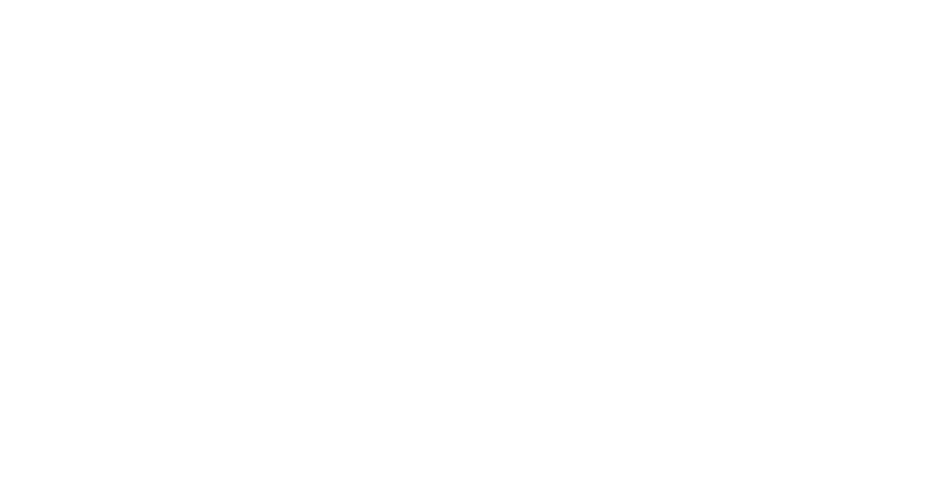
\includegraphics[width=12cm]{AcceleratorLattice-manual-logo.pdf} \\
\vskip 0.3in
\huge\bf David Sagan
\end{center}
}

\vfill
\break


%---------------------------------------------------------------------------------------------------

\cleardoublepage
\phantomsection 
\pdfbookmark[0]{Contents}{Contents}
\pdfbookmark[1]{Table of Contents}{toc} 
\tableofcontents

\cleardoublepage
\phantomsection 
\pdfbookmark[1]{List of Figures}{LoF} 
\listoffigures

\cleardoublepage
\phantomsection 
\pdfbookmark[1]{List of Tables}{LoT} 
\listoftables

%---------------------------------------------------------------------------------------------------
\setlength{\parskip}{\dPar}
\setlength{\parindent}{0ex}

%---------------------------------------------------------------------------------------------------
\part{Lattice Construction and Manipulation}
%---------------------------------------------------------------------------------------------------
\chapter{Introduction and Concepts}

%---------------------------------------------------------------------------
\section{Introduction}

This chapter is an introduction to, the \accellat package which is part of the
greater \scibmad ecosystem of toolkits and programs for accelerator simulations. With \accellat,
lattices can be constructed and manipulated. Essentially, a \vn{lattice} instance contains
a set of ``\vn{branches}'' and a branch contains 
an array of lattice \vn{elements} with each element representing an object like a magnet
or a RF cavity. A branch can be used to describe such
things as LINACs, storage rings, injection lines, X-ray beam lines, etc. Different branches in a
lattice can be connected together. For example, an injection line branch can be connected to a storage
ring branch or the lines of two rings can be connected together to form a colliding beam machine. 
This ability to describe the interconnections between branches means that 
a lattice instance can hold all the information about an entire machine complex from beam creation
to dump lines enabling a single lattice to be used as the basis of start-to-end simulations.

The sole purpose of the \accellat package is to implement methods for lattice construction.
Other stuff, like tracking and lattice analysis (for example, calculating
closed orbits and Twiss functions), is left to other packages in the \scibmad ecosystem.

%---------------------------------------------------------------------------
\section{Documentation}

There are three main sources of documentation of the \accellat package. 
One source is this PDF manual which gives in-depth documentationon. 
A second source is the web based introduction and overview guide.
Finally, functions, structs and other objects are documented in the code files themselves. 
Taking advantage of Julia's built-in documentation system, this code-file documentation 
can be accessed via using Julia's REPL.

%---------------------------------------------------------------------------
\section{Brief History}

\accellat has it's origins in the \bmad\cite{Sagan:Bmad2006} ecosystem of toolkits and programs 
developed over several decades at Cornell University.
While the development of \accellat is heavily influenced by the 
experience --- both good and bad --- of the development and use of \bmad as well as experience
with other accelerator simulation programs, the code of the two are
completely separate with \bmad being written in Fortran and \accellat being written in Julia.

The \julia language itself is used as the basis for constructing lattices with \accellat. 
Other simulation programs
have similarly utilized the underlying programming language for constructing 
lattices\cite{Appleby:Merlin2020,Iadarola:Xsuite2023}. This is in marked contrast to many accelerator
simulation programs such programs as MAD\cite{Grote:MAD1989}, Elegant\cite{Borland:Elegant2000}, and
Bmad. 
By using Julia for the lattice language, the user will automatically have access to such features 
as plotting, optimization packages, linear algebra packages, etc. 
This gives a massive boost to the versatility and usability of any \scibmad simulation program.
Moreover, maintainability is greatly enhanced due to the reduction in the amount of code that needs
to be developed.

%---------------------------------------------------------------------------------------------------
\section{Acknowledgements}

Thanks must go to the people who have contributed to this effort and without
whom \scibmad would only be a shadow of what it is today: 

\'Etienne Forest (aka Patrice Nishikawa),
Dan Abell,
Scott Berg,
Oleksii Beznosov,
Alexander Coxe,
Laurent Deniau,
Auralee Edelen,
Ryan Foussel,
Juan Pablo Gonzalez-Aguilera,
Georg Hoffstaetter,
Chris Mayes,
Matthew Signorelli,
Hugo Slepicka

%---------------------------------------------------------------------------
\section{Using AcceleratorLattice.jl}

\accellat is hosted on GitHub. The official repository is at
\begin{example}
  github.com/bmad-sim/AcceleratorLattice.jl
\end{example}
The \vn{README.md} file there has instructions on how to install \accellat.

A \vn{using} statement must be given before using \accellat in Julia
\begin{example}
  using AcceleratorLattice
\end{example}

%---------------------------------------------------------------------------
\section{Manual Conventions}
\label{s:manual.con}

This manual has the following conventions:
\begin{description}
%
\item[Type fields:]
\vn{Fields} of a type are also referred to as \vn{components} or \vn{parameters}.
A component \vn{c} of a type \vn{S} can be referred to as \vn{S.c}. In the case
of lattice elements, \vn{Ele} (the abstract type that all elements inherit from) is
used represent any of the subtypes such as \vn{Quadrupole}, etc. If the component
is an array, the notation \vn{S.c[]} can be used to emphasize this.
%
\end{description}

%---------------------------------------------------------------------------
\section{Lattice Elements}
\label{s:element.def}

The basic building block used to describe an accelerator is the lattice \vn{element}. An
element is generally something physical like a bending magnet or a
quadrupole, or a diffracting crystal. 

Lattice elements can be divided into two classes.
One class are the elements that particles are tracked through. These ``tracking'' elements are
contained in the ``tracking branches'' (\sref{s:branch.def}) of the lattice. Other elements, 
called ``\vn{lord}'' elements, are used to
represent relationships between elements. ``\vn{Super_lord}'' elements (\sref{c:super}) are
used when elements overlap spatially. ``\vn{Multipass_lord}'' elements (\ref{c:multipass})
are used when a beam goes through the same elements multiple times like in a recirculating Linac
or when different beam go through the same elements like in the interaction region of a
colliding beam machine.

%---------------------------------------------------------------------------
\section{Lattice Branches}
\label{s:branch.def}

The next level up from lattice \vn{elements} are the \vn{branches}.
Each branch holds an array of lattice elements. 
A branch is of type \vn{Branch}. 

There are two types of \vn{branches}: branches whose \vn{Branch.type} parameter is set to
a suitable subtype of \vn{LordBranch} holds Lord elements and 
branches whose \vn{Branch.type} parameter is set to \vn{TrackingBranch} holds an ordered
list of elements that can be tracked through. \accellat defines three lord branches named:
\begin{example}
  "super"       -- Contains super lord elements.
  "multipass"   -- Contains multipass lord elements.
  "girder"      -- Contains Girder elements.
\end{example}
Additional lord branches may be added by the user if desired.

A tracking branch can represent a LINAC, X-Ray beam line, storage ring, etc.
For all tracking branches, the first element in the element array
must be of type \vn{BeginningEle} (\sref{s:begin.ele}).
Additionally, for all tracking branches, 
the end element must be of type \vn{Marker} (\sref{s:mark}).

All tracking branches have a name \vn{Branch.name} inherited from the \vn{BeamLine} that defines
the branch in the lattice file and branches contains an array of elements \vn{Branch.ele[]}.
If the \vn{BeamLine} used to instantiate a tracking branch does not have a name, The default name
is used. The default name is \vn{"bN"} where \vn{N} is the index of the
branch in the \vn{Lattice.branch} array.

%---------------------------------------------------------------------------
\section{Lattices}
\label{s:lattice.def}

A \vn{lattice} (\sref{s:lattice.def}) is the root structure holding the information about a
``machine''. A machine may be as simple as a line of elements (like the elements of a Linac) or
as complicated as an entire accelerator complex with multiple storage rings, Linacs, transfer
lines, etc. All lattices are of type \vn{Lattice}.

Essentially, a \vn{lattice}, has an array \vn{Lattice.branch[]} of \vn{branches} with each branch 
describing part of the machine. 
Branches can be interconnected to form a unified whole.
Tracking branches can be interconnected using \vn{Fork} elements (\sref{s:fork}). 
This is used to simulate forking beam lines such as a connections to a transfer line, dump line, or an
X-ray beam line. The \vn{branch} from which other \vn{branches} fork but is not forked to by any
other \vn{branch} is called a \vn{root} branch.

A lattice may contain multiple \vn{root} \vn{branches}. For example, a pair of intersecting storage
rings will generally have two \vn{root} branches, one for each ring.

Branches can be accessed by name using the overloaded index operator for \vn{Lattice}. 
For example, if \vn{lat} is an instance of a lattice, the super lord branch (\sref{s:branch.def}),
which has the name \vn{"super"}, can be accessed via:
\begin{example}
  lat["super"]     # Access by branch name
  lat.branch[2]    # Access by branch index
\end{example}
Where it is assumed for this example that the super lord branch has index 2.

Similarly, lattice elements can be accessed by name or by index.
For example, if \vn{lat} is a lattice instance, and \vn{"q1"} is the name of an element or
elements that are in a branch named "b2", the following are equivalent:
\begin{example}
  elist = lat["q1"]
  elist = find(lat, "q1")
  b2 = lat.branch["b2"]; elist = b2["q1"]
\end{example}
\vn{elist} will be a vector of elements since a name may match to multiple elements.

%---------------------------------------------------------------------------
\section{AcceleratorLattice Conventions}
\label{s:conventions}

\accellat has the following conventions:
\begin{description}
%
\item[Evaluation is at upstream end:] 
For lattice element parameters that are s-dependent, the evaluation location is the
\vn{upstream} edge of the element (\sref{s:ref.construct}). These parameters include the 
element's floor position, the reference energy/momentum, and the s-position.
%
\end{description}

%---------------------------------------------------------------------------
\section{Minimal Working Lattice Example}
\label{s:min.lat}

The following is a minimal example of constructing a lattice with a quadrupole, drift, and then
a bend:
\begin{example}
  using AcceleratorLattice
  @ele begin_ele = BeginningEle(pc_ref = 1e7, species_ref = species("electron"))
  @ele q = Quadrupole(L = 0.6, K2 = 0.3)
  @ele d = Drift(L = 0.4)
  @ele b = Bend(L = 1.2, angle = 0.001)

  a_line = beamline("simple_line", [begin_ele, q, d, b])
  lat = Lattice("simple_lat", [a_line])
\end{example}

%---------------------------------------------------------------------------
\section{Differences From Bmad}

There are many differences between \accellat and \bmad. Many of of these will be fairly
obvious. Some differences to be aware of:
\begin{description}
\item
\bmad is generally case insensitive (except for things like file names). \accellat, like
the Julia language, is case sensitive.
%
With \bmad, the branch array within a lattice and the element array within a branch is
indexed from zero. With \scibmad, indexing of \vn{Lattice.branch[]} and \vn{branch.ele[]} is 
from one conforming to the Julia standard.
%
\item
The \bmad names for the coordinate systems (\sref{s:coords}) was somewhat different and not
always consistent. The \vn{floor} and \vn{element body} names are the same but \vn{machine}
coordinates are called the \vn{laboratory} in \bmad.
%
\item
Evaluation was at the downstream end (\sref{s:conventions}) in \bmad not the upstream end.
%
\item
With \bmad a value for any aperture limits of zero means the limit does not exist.
with \accellat a value of \vn{NaN} means the aperture does not exist. Additionally, with
\bmad a positive value for \vn{x1_limit} or \vn{y1_limit} meant that the aperture was
on the negative side of the \vn{x-axis} or \vn{y-axis} respectively. With \accellat, a positive
value for \vn{x_limit[1]} or \vn{y_limit[1]} means the aperture is on the positive side of 
of the \vn{x-axis} or \vn{y-axis} respectively. This makes the notation consistent across 
the different ways to specify apertures (compare with \vn{Mask} element syntax.).
%
\item
\accellat defines the reference point for misalignment of a Bend element as the center 
of the chord between the entrance and exit end points. 
With \bmad, the reference point is at the center of the reference trajectory arc between the entrance
and the exit. An additional difference is that the \bmad \vn{roll} misalignment is called \vn{tilt}
under \accellat.
%
\item
\bmad does not allow redefinition of named variables nor elements. \accellat allows this.
%
\item
With \bmad, the beginning and end elements are implicitly inserted into a branch line.
With \accellat, only an end element will be implicitly inserted if the end of the beamline is
not a marker. 
Also with \bmad the beginning element is always named \vn{Beginning} while with \accellat there
is no restriction on the name. 
%
\item
Restrictions on the order of statements used to create a lattice are different. 
For example, in \bmad, a statement defining a lattice element can be placed anywhere
except if there is an \vn{expand_lattice} statement and the element is not being used
with superposition in which case the element definition must be before the \vn{expand_lattice}
statement. With \accellat, element definitions must come before the element is used in a line.
%
\item
With \bmad superposition of two non-drift elements, if there existed the appropriate
combined type, will result in a \vn{super_slave} of the appropriate combined type. For example,
a \vn{solenoid} superimposed over a \vn{quadrupole} would give a \vn{sol_quad} \vn{super_slave} with
\vn{solenoid} and \vn{quadrupole} \vn{super_lords}. The problem here is that calculation of the
\vn{super_slave} parameters may not be possible. For example if the \vn{super_lord}
elements are misaligned, in general it is not possible to compute a corresponding \vn{super_slave}
misalignment. To avoid this, \accellat creates a \vn{UnionEle} \vn{super_slave} element
(which in \bmad is known as a ``jumbo'' \vn{super_slave}). It is up to the tracking routines to
figure out how to track though a \vn{UnionEle}
%
\item
In \vn{Bmad} there are two types of bends called \vn{sbend} and \vn{rbend}. 
This organization was inherited from \vn{MAD}. While both \vn{sbends} and \vn{rbends}
represent the same physical type of bend, the two have different ways to specify the bend parameters. 
This can be confusing since \vn{rbends} and \vn{sbends} use the same names for different parameters.
For example, the length \vn{l} for an \vn{sbend} is the arc length but for an \vn{rbend} it is the
chord length. To avoid confusion, \accellat combines the two into a single \vn{Bend} type with
distinct parameter names. For example, \vn{L} is the arc length and \vn{L_chord} is the chord length.
\end{description}




\chapter{Lattice Elements}
\label{c:ele}

This chapter discusses lattice elements including how to create them and how to manipulate them.

%---------------------------------------------------------------------------------------------------
\section{Element Types}
\label{s:ele.types}

Lattice element types (\vn{Quadrupole}, \vn{RFCavity}, etc.) are structs that inherit from the abstract 
type \vn{Ele}. Lattice elements documentation is in chapter~\sref{c:ele.types}. 
In the REPL, to see a list of all element types, use the command \vn{subtypes(Ele)}:
\begin{example}
  julia> subtypes(Ele)
  41-element Vector\{Any\}:
   ACKicker
   BeamBeam
   BeginningEle
   Bend
   ...
\end{example}

%---------------------------------------------------------------------------------------------------
\section{Instantiating a Lattice Element}
\label{s:ele.def}

Elements are defined using the \vn{@ele} or \vn{@eles} macros. 
The general syntax of the \vn{@ele} macro is:
\begin{example}
  @ele eleName = eleType(param1 = val1, param2 = val2, ...)
\end{example}
where \vn{eleName} is the name of the element, \vn{eleType} is the type of element, 
\vn{param1}, \vn{param2},
etc. are parameter names and \vn{val1}, \vn{val2}, etc. are the parameter values.
Example:
\begin{example}
  @ele qf = Quadrupole(L = 0.6, Kn1 = 0.370)
\end{example}
The \vn{@ele} macro will construct a \julia variable with the name \vn{eleName}. 
Additionally, the element
that this variable references will also hold \vn{eleName} as the name of the element. So with this
example, \vn{qf.name} will be the string \vn{"qf"}. If multiple elements are being defined in a 
group, a single
\vn{@eles} macro can be used instead of multiple \vn{@ele} macros using the syntax:
\begin{example}
  @eles begin
    eleName1 = eleType1(p11 = v11, p12 = v12, ...)
    eleName2 = eleType2(p21 = v21, p22 = v22, ...)
    ... etc...
  end
\end{example}
Example:
\begin{example}
  @eles begin
    s1 = Sextupole(L = ...)
    b2 = Bend(...)
    ...
  end
\end{example}

%---------------------------------------------------------------------------------------------------
\section{Element Parameter Groups}
\label{s:ele.groups}

Generally, element parameters are grouped into ``\vn{element} \vn{parameter} \vn{group}'' 
structs which inherit from the abstract type \vn{EleParameterGroup}. 
Element parameter documentation is in Chapter~\sref{c:ele.groups}. In the REPL,
To see a list of parameter groups, use the \vn{suptypes} function:
\begin{example}
  julia> subtypes(EleParameterGroup)
  28-element Vector{Any}:
   BodyShiftGroup
   ApertureGroup
   BMultipoleGroup
   ...
\end{example}
Chapter~\sref{c:ele.types} documents the parameters groups that are associated with any particular element type.
In the REPL, the associated parameter groups can be viewed using Julia's help function. Example: 
\begin{example}
  help?> Quadrupole
    mutable struct Quadrupole <: Ele
    Type of lattice element.

    Associated parameter groups
    ===========================
      •  BodyShiftGroup -> Element position/orientation shift.
      •  ApertureGroup -> Vacuum chamber aperture.
      •  BMultipoleGroup -> Magnetic multipoles.
      •  EMultipoleGroup -> Electric multipoles.
      •  OrientationGroup -> Floor position and orientation.
      •  LengthGroup -> Length and s-position parameters.
      •  LordSlaveGroup -> Element lord and slave status.
      •  MasterGroup -> Contains field_master parameter.
      •  ReferenceGroup -> Reference energy and species.
      •  DescriptionGroup -> String labels for element.
      •  TrackingGroup -> Default tracking settings.
\end{example}
Alternatively, 

%---------------------------------------------------------------------------------------------------
\section{Element Parameters}
\label{s:ele.params}

For example, the \vn{LengthGroup} holds the length and s-positions of the element and is defined by:
\begin{example}
  @kwdef struct LengthGroup <: EleParameterGroup
    L::Number = 0.0               # Length of element
    s::Number = 0.0               # Starting s-position
    s_downstream::Number = 0.0    # Ending s-position
    orientation::Int = 1          # Longitudinal orientation
  end
\end{example}
The \vn{@kwdef} macro automatically defines a keyword-based constructor for \vn{LengthGroup}.
See the Julia manual for more information on \vn{@kwdef}. 
To see a list of all element parameter groups use the \vn{subtypes(EleParamterGroup)} command.
To see the components of a given group use the \vn{fieldnames} function. For information on
a given element parameter use the \vn{info(::Symbol)} function where the argument is the
symbol corresponding to the component. For example, the information on
the \vn{s_downstream} parameter which is a field of the \vn{LengthGroup} is:
\begin{example}
  julia> info(:s_downstream)
    User name:       s_downstream
    Stored in:       LengthGroup.s_downstream
    Parameter type:  Number
    Units:           m
    Description:     Longitudinal s-position at the downstream end.
\end{example}
Notice that the argument to the \vn{info} function is the symbol associated with the parameter.
the ``user name'' is the name used when setting the parameter. For instance, if \vn{q} is a
lattice element, \vn{q.s_downstream} would be used to access the \vn{s_downstream} component of \vn{q}.
This works, even though \vn{s_downstream} is not a direct component of an element, since the dot
selection operator for lattice elements has been overloaded as explained in \sref{s:ele.access}.
For most parameters, the user name and the name of the corresponding component in the element parameter
group are the same. However, there are exceptions. For example:
\begin{example}
  julia> info(:theta)
    User name:       theta_floor
    Stored in:       OrientationGroup.theta
    Parameter type:  Number
    Units:           rad
    Description:     Element floor theta angle orientation
\end{example}
In this example, the user name is \vn{theta_floor} so that this parameter can be set via
\begin{example}
  @ele bg = BeginningEle(theta_floor = 0.3)    # Set at element definition time.
  bg.theta_floor = 2.7                         # Or set after definition.
\end{example}
But the component in the \vn{OrientationGroup} is \vn{theta} so
\begin{example}
  bg.OrientationGroup.theta = 2.7   # Equivalent to the set above.
\end{example}

%---------------------------------------------------------------------------------------------------
\section{How Element Parameters are Stored in an Element}
\label{s:ele.access}

All lattice element types have a single field of type \vn{Dict\{Symbol,Any\}} named \vn{pdict}.
The values of \vn{pdict} will, with a few exceptions, be an
element parameter group. The corresponding key for a parameter group in \vn{pdict} is the symbol associated 
with the type. For example, a \vn{LengthGroup} struct would be stored in \vn{pdict[:LengthGroup]}.

To (partially) hide the complexity of parameter groups, the dot selection operator is overloaded for elements.
This is achieved by overloading the \vn{Base.setproperty} and \vn{Base.getproperty} functions, 
which get called when the dot selection operator is used.
For example, if \vn{q} is an element instance, \vn{q.s} will get mapped to \vn{q.pdict[:LengthGroup].s}.
Additionally, \vn{q.LengthGroup} is mapped to \vn{q.pdict[:LengthGroup]}.

Besides simplifying the syntax, overloading the dot selection operator has a second purpose which
is to allow the \accellat bookkeeping routines to properly do dependent parameter bookkeeping (\sref{param.depend}).
To illustrate this, consider the following two statements which both set the \vn{s_downstream}
parameter of an element named \vn{q1}:
\begin{example}
  q1.pdict[:Length_group].s_downstream = q1.pdict[:Length_group].s + 
                                                     q1.pdict[:Length_group].L
  q1.s_downstream = q1.s + q1.L
\end{example}
These two statements are not equivalent. The difference is that in the first statement when
\vn{setproperty} is called to handle \vn{q1.pdict}, the code will simply return \vn{q1.pdict} 
(the code knows that \vn{pdict} is special) and do nothing else. 
However, with the second statement, \vn{setproperty} not only sets
\vn{q1.s_downstream} but additionally records the set by adding an entry to
\vn{q1.pdict[:changed]} which is a dict within \vn{pdict}. 
The key of the entry will, in this case, be the symbol \vn{:s_downstream} 
and the value will be the old value of the parameter. 
When the \vn{bookkeeper(::Lattice)} function is called (\sref{xxx}), the bookkeeping code will use the
entries in \vn{ele.pdict[:changed]} to limit the bookkeeping to what is necessary and thus
minimize computation time. 
Knowing what has been changed is also important in resolving what
dependent parameters need to be changed. 
For example, if the bend \vn{angle} is changed, the bookkeeping code will set the 
bending strength \vn{g} using the equation \vn{g} = \vn{angle} / \vn{L}. If, instead,
\vn{g} is changed, the bookkeeping code will set \vn{angle} appropriately. 

While the above may seem complicated, in practice the explicit use of \vn{q1.pdict} should be avoided
since it prevents the bookkeeping from dealing with dependent parameters.
The place where \vn{q1.pdict} is needed is in the bookkeeping code itself to avoid infinite loops.
 

%---------------------------------------------------------------------------------------------------
\section{Bookkeeping and Dependent Element Parameters}
\label{s:param.depend}

After lattice parameters are changed, the function \vn{bookkeeper(::Lattice)} needs to be called
so that dependent parameters can be updated. 
Since bookkeeping can take a significant amount of time if bookkeeping is done every time
a change to the lattice is made, and since there is no good way to tell when bookkeeping should
be done, After lattice expansion, \vn{bookkeeper(::Lattice)} is never called directly by \accellat 
functions and needs to be called by the User when appropriate (generally before tracking or
other computations are done).

Broadly, there are two types of dependent parameters: intra-element dependent parameters where
the changed parameters and the dependent parameters are all within the same element and
cascading dependent parameters where changes to one element cause changes to parameters of 
elements downstream.

The cascading dependencies are:
\begin{description}
%
\item [s-position dependency:]
Changes to an elements length \vn{L} or changes to the beginning element's \vn{s} parameter will
result in the s-positions of all downstream elements changing.
%
\item [Reference energy dependency:] Changes to the be beginning element's reference energy (or
equivilantly the referece momentum), or changes to the \vn{voltage} of an \vn{LCavity} element
will result in the reference energy of all downstream elements changing.
%
\item[Floor position dependency:]
The position of a lattice element in the floor coordinate system (\sref{s:floor}) is affected
by a) the lengths of all upstream elements, b) the bend angles of all upstream elements, and c)
the position in floor coordinates of the beginning element.
\end{description}


%---------------------------------------------------------------------------------------------------
\section{Defining a New Element Type}
\label{s:ele.new.type}

To construct a new type, use the \vn{@construct_ele_type} macro. Example:
\begin{example}
  @construct_ele_type MyEle
\end{example}
And this defines a new type called \vn{MyEle} which inherits from the abstract type \vn{Ele} and
defines \vn{MyEle} to have a single field called \vn{pdict} which is of type \vn{Dict\{Symbol,Any\}}.
This macro also pushes the name

%---------------------------------------------------------------------------------------------------
\section{Defining New Element Parameters}
\label{s:ele.new.param}


\chapter{Lattice Element Types}
\label{c:ele.types}

%---------------------------------------------------------------------------------------------------

This chapter discusses the various types of elements
available in \accellat.
Table~\ref{t:particle.classes} lists the elements that can be tracked through.
Table~\ref{t:control.classes} lists the \vn{controller} element types that can be used for parameter
control of other elements. 

\begin{table}[htb]
\centering
{\tt
\begin{tabular}{llll} \toprule
  {\it Element}    & {\it Section}         & {\it Element}      & {\it Section}       \\ \midrule
  BeamBeam         & \ref{s:beambeam}      &  LCavity           & \ref{s:lcav}        \\
  BeginningEle     & \ref{s:begin.ele}     &  Marker            & \ref{s:marker}      \\
  Bend             & \ref{s:bend}          &  Mask              & \ref{s:mask}        \\
  Collimator       & \ref{s:col}           &  Match             & \ref{s:match}       \\ 
  CrabCavity       & \ref{s:crab}          &  NullEle           & \ref{s:nullele}     \\
  Custom           & \ref{s:custom}        &  Octupole          & \ref{s:oct}         \\
  Drift            & \ref{s:drift}         &  Patch             & \ref{s:patch}       \\  
  EGun             & \ref{s:egun}          &  Quadrupole        & \ref{s:quad}        \\ 
  ElSeparator      & \ref{s:elsep}         &  RFCavity          & \ref{s:rfcav}       \\ 
  EMField          & \ref{s:emfield}       &  Sextupole         & \ref{s:sex}         \\ 
  Fiducial         & \ref{s:fiducial}      &  Solenoid          & \ref{s:sol}         \\
  FloorShift       & \ref{s:floorshift}    &  Taylor            & \ref{s:taylor}      \\
  Foil             & \ref{s:foil}          &  ThickMultipole    & \ref{s:thickmult}   \\
  Fork             & \ref{s:fork}          &  Undulator         & \ref{s:undulator}   \\
  Instrument       & \ref{s:instrument}    &  UnionEle          & \ref{s:unionele}    \\
  Kicker           & \ref{s:kicker}        &  Wiggler           & \ref{s:wiggler}     \\
  \bottomrule
\end{tabular}
} 
\caption{Table of non-controller element types.}
\label{t:particle.classes}
\end{table}

\begin{table}[ht]
\centering
{\tt
\begin{tabular}{llll} \toprule
  {\it Element}  & {\it Section}     & {\it Element}  & {\it Section}    \\ \midrule
  Controller     & \ref{s:control}     &  Ramper        & \ref{s:ramper}   \\
  Girder         & \ref{s:girder}    &                &                  \\
 \\ \bottomrule
\end{tabular}
}
\caption{Table of controller elements.}
\label{t:control.classes}
\end{table}

\newpage

%-----------------------------------------------------------------
\section{BeamBeam}
\label{s:beambeam}


%-----------------------------------------------------------------
\section{BeginningEle}
\label{s:begin.ele}

A \vn{BeginningEle} element must be present as the first element of every tracking branch.
(\sref{s:branch.def}).

Element parameter groups associated with a \vn{BeginningEle} are:
\begin{example}
  LengthGroup          -> Length and s-position parameters.
  LordSlaveGroup       -> Element lord and slave status.
  StringGroup          -> Informational strings.
  ReferenceGroup       -> Reference energy and species.
  FloorPositionGroup   -> Global floor position and orientation.
  TrackingGroup        -> Default tracking settings.
\end{example}

\newpage

%-----------------------------------------------------------------
\section{Bend Element}
\label{s:bend}

A \vn{Bend} type element represents a dipole bend. 

%-----------------------------------------------------------------
\section{Collimator}
\label{s:collimator}


%-----------------------------------------------------------------
\section{CrabCavity}
\label{s:crab}


%-----------------------------------------------------------------
\section{Custom}
\label{s:custom}


%-----------------------------------------------------------------
\section{Drift}
\label{s:drift}


%-----------------------------------------------------------------
\section{EGun}
\label{s:egun}


%-----------------------------------------------------------------
\section{ElSeparator}
\label{s:elsep}


%-----------------------------------------------------------------
\section{EMField}
\label{s:emfield}


%-----------------------------------------------------------------
\section{Fiducial}
\label{s:fiducial}


%-----------------------------------------------------------------
\section{FloorShift}
\label{s:floorshift}


%-----------------------------------------------------------------
\section{Foil}
\label{s:foil}


%-----------------------------------------------------------------
\section{Fork}
\label{s:fork}


%-----------------------------------------------------------------
\section{Instrument}
\label{s:instrument}


%-----------------------------------------------------------------
\section{Kicker}
\label{s:kicker}


%-----------------------------------------------------------------
\section{LCavity}
\label{s:lcav}


%-----------------------------------------------------------------
\section{Marker}
\label{s:marker}


%-----------------------------------------------------------------
\section{Match}
\label{s:match}


%-----------------------------------------------------------------
\section{NullEle}
\label{s:nullele}


%-----------------------------------------------------------------
\section{Octupole}
\label{s:oct}


%-----------------------------------------------------------------
\section{Patch}
\label{s:patch}


%-----------------------------------------------------------------
\section{Quadrupole}
\label{s:quad}


%-----------------------------------------------------------------
\section{RFCavity}
\label{s:rfcav}


%-----------------------------------------------------------------
\section{Sextupole}
\label{s:sex}


%-----------------------------------------------------------------
\section{Taylor}
\label{s:taylor}


%-----------------------------------------------------------------
\section{ThickMultipole}
\label{s:thickmult}


%-----------------------------------------------------------------
\section{Undulator}
\label{s:undulator}


%-----------------------------------------------------------------
\section{UnionEle}
\label{s:unionele}


%-----------------------------------------------------------------
\section{Wiggler}
\label{s:wiggler}



\chapter{Enums and Holy Traits}
\label{c:enums}

Enums (\sref{s:enums}) and Holy traits (\sref{s:holy}) are used to define ``switches'' which are
variables whose value can be one of a set of named constants. 
A web search will provide documentation. 

The advantage of Holy traits is that they can be used with function dispatch. The disadvantage is
that the same Holy trait value name cannot be used with multiple groups. Generally, if function
dispatch is not needed (which is true for the majority of cases), switch groups are defined using enums.

%---------------------------------------------------------------------------------------------------
\section{Enums}
\label{s:enums}

\accellat uses the package \vn{EnumX.jl} to define enums (enumerated numbers).
Essentially what happens is that for each enum group there is a group name, For example \vn{BendType},
along with a set of values which, for \vn{BendType}, is \vn{SECTOR} and \vn{RECTANGULAR}. Values
are always referred to by their "full" name which in this example is \vn{BendType.SECTOR} and
\vn{BendType.RECTANGULAR}. Exception: \vn{BranchGeometry.CLOSED} and \vn{BranchGeometry.OPEN} are
used often enough so that the constants \vn{OPEN} and \vn{CLOSED} are defined.

The group name followed by a \vn{.T} suffix denotes the enum type.
For example:
\begin{example}
  struct ApertureGroup <: EleParameterGroup
    aperture_type::ApertureShape.T = ApertureShape.ELLIPTICAL
    aperture_at::BodyLoc.T = BodyLoc.ENTRANCE_END
    ...
\end{example}

The \vn{enum} function is used to convert a list into an enum group and export the names.
The \vn{enum} function also overloads \vn{Base.string} so that something like \vn{string(Lord.NOT)} 
will return \vn{"Lord.NOT"} instead of just \vn{"NOT"} (an issue with the EnumX.jl package). 
See the documentation for \vn{enum} for more details.

The \vn{enum_add} function is used to add values to an existing enum group. See the documentation for
\vn{enum_add} for more details. This function is used with code extensions to customize \accellat.

The enum groups are:
\begin{table}[htb]
\centering
{\tt
\begin{tabular}{llll} \toprule
  {\it Group}       & {\it Section}             & {\it Group}         & {\it Section}       \\ \midrule
  BendType          & \sref{s:bendtype}         & Slave               & \sref{s:slave.enum} \\
  BodyLoc           & \sref{s:bodyloc}          & Loc                 & \sref{s:loc}        \\
  BranchGeometry    & \sref{s:branchgeometry}   & Select              & \sref{s:select}     \\
  Cavity            & \sref{s:cavity}           & ExactMultipoles     & \sref{s:exactmultipoles} \\
  Lord              & \sref{s:lord.enum}        & FiducialPt          & \sref{s:fiducialpt} \\
  ParticleState     & \sref{s:particlestate}    &                     &                     \\
  \bottomrule
\end{tabular}
} 
\caption{Table of enum groups.}
\label{t:enum}
\end{table}
%---------------------------------------------------------------------------------------------------
\subsection{BendType Enum Group}
\label{s:bendtype}
\vspace*{-2ex}

Type of Bend element. Possible values: \\
\vspace*{-0.5ex} \\
\begin{tabular}{ll}
  BendType &  \\
  \indnt .SECTOR      & -- Sector shape \\
  \indnt .RECTANGULAR & -- Rectangular shape \\
\end{tabular} 
\hfill \break \vskip -1.2ex

\vn{BendType} is used with the \vn{bend_type} parameter of the \vn{BendGroup} parameter group
(\sref{s:bend.g}). The \vn{bend_type} parameter gives the ``logical'' shape of the bend.
The setting of \vn{bend_type} is only relavent when the bend curvature is varied.
See \sref{s:bend.g} for more details.

%---------------------------------------------------------------------------------------------------
\subsection{BodyLoc Enum Group}
\label{s:bodyloc}
\vspace*{-2ex}

Longitudinal location with respect to an element's body coordinates.
Possible values:\\
\vspace*{-0.5ex} \\
\begin{tabular}{ll}
  BodyLoc & \\
  \indnt .ENTRANCE_END & -- Body entrance end \\
  \indnt .CENTER       & -- Element center \\
  \indnt .EXIT_END     & -- Body exit end \\
  \indnt .BOTH_ENDS    & -- Both ends \\
  \indnt .NOWHERE      & -- No location \\
  \indnt .EVERYWHERE   & -- Everywhere \\
\end{tabular}
\hfill \break \vskip -1.2ex

\vn{BodyLoc} enums are are useful to locate things that are ``attached'' to an element.
For example, specifying where apertures are placed.

%---------------------------------------------------------------------------------------------------
\subsection{BranchGeometry Enum Group}
\label{s:branchgeometry}
\vspace*{-2ex}

Geometry of a lattice branch. Used for setting a branche's \vn{geometry} parameter. 
Possible values:\\
\vspace*{-0.5ex} \\
\begin{tabular}{ll}
  BranchGeometry & \\
  \indnt .OPEN    & -- Open geometry like a Linac. Default \\
  \indnt .CLOSED  & -- Closed geometry like a storage ring.
\end{tabular}
\hfill \break \vskip -1.2ex

A branch with a \vn{CLOSED} geometry is something like a storage ring where the particle beam
recirculates through the machine. A branch with an \vn{OPEN} geometry is something like a linac.
In this case, the initial Twiss parameters need to be
specified at the beginning of the branch. If the
\vn{geometry} is not specified, \vn{OPEN} is the default.

Since the geometry is widely used, \vn{OPEN} and \vn{CLOSED} have been defined and
can be used in place of \vn{BranchGeometry.OPEN} and \vn{BranchGeometry.CLOSED}.

Notice that by specifying a \vn{CLOSED} geometry, it does {\em not} mean that the downstream end of
the last element of the branch has the same floor coordinates (\sref{s:floor}) as the floor
coordinates at the beginning. Setting the geometry to \vn{CLOSED} simply signals to a program to
compute the periodic orbit and periodic Twiss parameters as opposed to calculating orbits and Twiss
parameters based upon initial orbit and Twiss parameters given at the beginning of the branch.  Indeed,
it is sometimes convenient to treat branches as closed even though there is no closure in the floor
coordinate sense. For example, when a machine has a number of repeating ``periods'', it may be
convenient to only use one period in a simulation. Since \accellat ignores closure in the floor
coordinate sense, it is up to the lattice designer to ensure that a branch is truly geometrically
closed if that is desired.

%---------------------------------------------------------------------------------------------------
\subsection{Cavity Enum Group}
\label{s:cavity}
\vspace*{-2ex}

Type of RF cavity.
Possible values:\\
\vspace*{-0.5ex} \\
\begin{tabular}{ll}
  Cavity & \\
  \indnt .STANDING_WAVE   & -- Standing wave cavity \\
  \indnt .TRAVELING_WAVE  & -- Traveling wave cavity \\
\end{tabular}
\hfill \break \vskip -1.2ex

%---------------------------------------------------------------------------------------------------
\subsection{ParticleState Enum Group}
\label{s:particlestate}

State of a particle.
Possible values:\\
\vspace*{-0.5ex} \\
\begin{tabular}{ll}
  ParticleState & \\
  \indnt .PREBORN     & -- State before emission from cathode.  \\
  \indnt .ALIVE       & -- Alive and kicking.  \\
  \indnt .LOST        & -- Particle has been lost.  \\
  \indnt .LOST_NEG_X  & -- Hit aperture in the -x direction.  \\
  \indnt .LOST_POS_X  & -- Hit aperture in the +x direction.  \\
  \indnt .LOST_NEG_Y  & -- Hit aperture in the -y direction.  \\
  \indnt .LOST_POS_Y  & -- Hit aperture in the +y direction.  \\
  \indnt .LOST_PZ     & -- Lost all forward momentum.   \\
  \indnt .LOST_Z      & -- Out of RF bucket.  \\
\end{tabular}
\hfill \break \vskip -1.2ex

The \vn{LOST} value is used when it is not possible to assign the particle state to one of the
other lost values.

The \vn{.LOST_PZ} value is used by $s$ (longitudinal position) based trackers which are not
able to handle particles changing their longitudinal motion direction. For tracking something
like dark current electrons which can go back and forth longitudinally, a time based tracker
is needed.

%---------------------------------------------------------------------------------------------------
\subsection{Loc Enum Group}
\label{s:loc}
\vspace*{-2ex}

Longitudinal location with respect to element's branch coordinates.
Possible values: \\
\vspace*{-0.5ex} \\
\begin{tabular}{ll}
  Loc & \\
  \indnt .UPSTREAM_END   & -- Upstream element end \\
  \indnt .CENTER         & -- center of element \\
  \indnt .INSIDE         & -- Somewhere inside \\
  \indnt .DOWNSTREAM_END & -- Downstream element end \\
\end{tabular}
\hfill \break \vskip -1.2ex


%---------------------------------------------------------------------------------------------------
\subsection{Select Enum Group}
\label{s:select}
\vspace*{-2ex}

Specifies where to select if there is a choice of elements or positions.
Possible values:\\
\vspace*{-0.5ex} \\
\begin{tabular}{ll}
  Select & \\
  \indnt .UPSTREAM   & -- Select upstream \\
  \indnt .DOWNSTREAM & -- Select downstream \\
\end{tabular}
\hfill \break \vskip -1.2ex


%---------------------------------------------------------------------------------------------------
\subsection{ExactMultipoles Enum Group}
\label{s:exactmultipoles}
\vspace*{-2ex}

How multipoles are handled in a Bend element.
Possible values:\\
\vspace*{-0.5ex} \\
\begin{tabular}{ll}
  ExactMultipoles & \\
  \indnt .OFF               & -- Bend curvature not taken into account. \\
  \indnt .HORIZONTALLY_PURE & -- Coefficients correspond to horizontally pure multipoles. \\
  \indnt .VERTICALLY_PURE   & -- Coefficients correspond to vertically pure multipoles. \\
\end{tabular}
\hfill \break \vskip -1.2ex


%---------------------------------------------------------------------------------------------------
\subsection{FiducialPt Enum Group}
\label{s:fiducialpt}
\vspace*{-2ex}

Fiducial point location with respect to element's branch coordinates.
Possible values:\\
\vspace*{-0.5ex} \\
\begin{tabular}{ll}
  FiducialPt & \\
  \indnt .ENTRANCE_END & -- Entrance end of element \\
  \indnt .CENTER       & -- Center of element \\
  \indnt .EXIT_END     & -- Exit end of element \\
  \indnt .NONE         & -- No point chosen \\
\end{tabular}


%---------------------------------------------------------------------------------------------------
\section{Holy Traits}
\label{s:holy}

\vn{Holy traits} (named after Tim Holy) are a design pattern in Julia that behave similarly
to \vn{enums} (\sref{s:enum}). A Holy trait group consists of a base abstract type with a set of values
(traits) which are abstract types that inherit from the base abstract type.

The advantage of Holy traits is that they can be used with function dispatch. The disadvantage is
that the same Holy trait value name cannot be used with multiple groups.

There is a convenience function \vn{holy_traits} which will define a traits group, export the names,
and create a docstring for the group. Values can be added to an existing group by defining a 
new struct that inherits from the group abstract type.

Example: To extend the \vn{EleGeometry} trait group to include the value \vn{HELIX_GEOMETRY} do
\begin{example}
  abstract type HELIX_GEOMETRY <: EleGeometry
\end{example}

%---------------------------------------------------------------------------------------------------
\subsection{ApertureShape Holy Trait Group}
\label{s:apertureshape}
\vspace*{-2ex}

The shape of an aperture.\\
\vspace*{-0.5ex} \\
\begin{tabular}{ll}
  RECTANGULAR   & -- Rectangular shape. \\
  ELLIPTICAL    & -- Elliptical shape. \\
  VERTEX        & -- Shape defined by set of vertices. \\
  CUSTOM_SHAPE  & -- Shape defined with custom function. \\
\end{tabular}
\hfill \break \vskip -1.2ex

%---------------------------------------------------------------------------------------------------
\subsection{EleGeometry Holy Trait Group}
\label{s:elegeometry}
\vspace*{-2ex}

The geometry of the reference orbit through an element. \\
\vspace*{-0.5ex} \\
\begin{tabular}{ll}
  STRAIGHT          & -- Straight line geometry. \\
  CIRCULAR          & -- Circular "bend-like" geometry. \\
  ZERO_LENGTH       & -- Zero longitudinal length geometry. \\
  PATCH_GEOMETRY    & -- Patch element like geometry. \\
  GIRDER_GEOMETRY   & -- Support girder-like geometry. \\
  CRYSTAL_GEOMETRY  & -- Crystal geometry. \\
  MIRROR_GEOMETRY   & -- Mirror geometry. \\
\end{tabular}
\hfill \break \vskip -1.2ex


\chapter{Element Parameter Groups}
\label{c:ele.groups}

Generally, element parameters are grouped into ``\vn{element} \vn{parameter} \vn{group}'' 
types which is discussed in \sref{c:ele}.

Element parameter groups inherit from the abstract type \vn{EleParameterGroup} which
in turn inherits from \vn{BaseEleParameterGroup}. Some
parameter groups have sub-group components. 
These sub-groups also inherit from \vn{BaseEleParameterGroup}:
\begin{example}
  abstract type BaseEleParameterGroup end
  abstract type EleParameterGroup <: BaseEleParameterGroup end
  abstract type EleParameterSubGroup <: BaseEleParameterGroup end
\end{example}

All parameter groups have associated docstrings that can be accessed when using the REPL.

The parmeters groups are:
\begin{table}[htb]
\centering
{\tt
\begin{tabular}{llll} \toprule
  {\it Group}        & {\it Section}         & {\it Group}      & {\it Section}         \\ \midrule
 AlignmentGroup      & \sref{s:align.g}      & LordSlaveGroup      & \sref{s:lord.slave.g} \\
 ApertureGroup       & \sref{s:apert.g}      & MasterGroup         & \sref{s:master.g}     \\
 BMultipoleGroup     & \sref{s:bmult.g}      & PatchGroup          & \sref{s:patch.g}      \\ 
 BeamBeamGroup       & \sref{s:bb.g}         & RFFieldGroup        & \sref{s:rffield.g}    \\
 BendGroup           & \sref{s:bend.g}       & RFGroup             & \sref{s:rf.g}         \\ 
 EMultipoleGroup     & \sref{s:emult.g}      & RFMasterGroup       & \sref{s:rfmaster.g}   \\
 FloorPositionGroup  & \sref{s:floor.g}      & ReferenceGroup      & \sref{s:ref.g}        \\
 GirderGroup         & \sref{s:girder.g}     & SolenoidGroup       & \sref{s:sol.g}        \\
 InitParticleGroup   & \sref{s:initp.g}      & StringGroup         & \sref{s:string.g}     \\
 LCavityGroup        & \sref{s:lcav.g}       & TrackingGroup       & \sref{s:track.g}      \\
 LengthGroup         & \sref{s:length.g}     & TwissGroup          & \sref{s:twiss.g}      \\ 
  \bottomrule
\end{tabular}
} 
\caption{Table of element parameter groups.}
\label{t:particle.groups}
\end{table}


* Note: NaN denotes parameter that is not set.

* beta_ref is a dependent attribute.



 




%---------------------------------------------------------------------------------------------------
\section{Enums}
\label{s:enums}

\accellat uses the package \vn{EnumX.jl} to define enums (enumerated numbers).
Essentially what happens is that for each enum group there is a group name, For example \vn{BendType},
along with a set of values which, for \vn{BendType}, is \vn{SECTOR} and \vn{RECTANGULAR}. Values
are always referred to by their "full" name which in this example is \vn{BendType.SECTOR} and
\vn{BendType.RECTANGULAR}. Exception: \vn{BranchGeometry.CLOSED} and \vn{BranchGeometry.OPEN} are
used often enough so that the constants \vn{OPEN} and \vn{CLOSED} are defined.

The group name followed by a \vn{.T} suffix denotes the enum type.
For example:
\begin{example}
  struct ApertureGroup <: EleParameterGroup
    aperture_type::ApertureShape.T = ApertureShape.ELLIPTICAL
    aperture_at::BodyLoc.T = BodyLoc.ENTRANCE_END
    ...
\end{example}

The \vn{enum} function is used to convert a list into an enum group and export the names.
The \vn{enum} function also overloads \vn{Base.string} so that something like \vn{string(Lord.NOT)} 
will return \vn{"Lord.NOT"} instead of just \vn{"NOT"} (an issue with the EnumX.jl package). 
See the documentation for \vn{enum} for more details.

The \vn{enum_add} function is used to add values to an existing enum group. See the documentation for
\vn{enum_add} for more details. This function is used with code extensions to customize \accellat.


Below is a list of enum groups defined in \accellat. 
\begin{description}
%
\item[BendType] --- Type of Bend element magnet.\Newline
\hspace*{-20pt}
\begin{tabular}{ll}
  SECTOR      & --- Sector shape\\
  RECTANGULAR & --- Rectangular shape \\
\end{tabular}
%
\item[BodyLoc] --- Longitudinal location with respect to element's body coordinates.\Newline
\hspace*{-20pt}
\begin{tabular}{ll}
  ENTRANCE_END & --- Body entrance end \\
  CENTER       & --- Element center \\
  EXIT_END     & --- Body exit end \\
  BOTH_ENDS    & --- Both ends \\
  NOWHERE      & --- No location \\
  EVERYWHERE   & --- Everywhere \\
\end{tabular}
%
\item[BranchGeometry] --- Geometry of a lattice branch\Newline
\hspace*{-20pt}
\begin{tabular}{ll}
  OPEN    & --- Open geometry like a Linac. \\
  CLOSED  & --- Closed geometry like a storage ring.
\end{tabular}
%
\item[Cavity] --- Type of RF cavity. \Newline
\hspace*{-20pt}
\begin{tabular}{ll}
  STANDING_WAVE   & --- Standing wave cavity \\
  TRAVELING_WAVE  & --- Traveling wave cavity \\
\end{tabular}
%
\item[Lord] --- Type of lord an element is \Newline
\hspace*{-20pt}
\begin{tabular}{ll}
  NOT       & --- Not a lord \\
  SUPER     & --- Super lord \\
  MULTIPASS & --- Multipass lord \\
  GOVERNOR  & --- Girder and other "minor" lords \\ 
\end{tabular}
%
\item[Slave] --- Type of slave an element is \Newline
\hspace*{-20pt}
\begin{tabular}{ll}
  NOT       & --- Not a slave \\
  SUPER     & --- Super slave \\
  MULTIPASS & --- Multipass slave \\
\end{tabular}
%
\item[Loc] --- Longitudinal location with respect to element's machine coordinates. \Newline
\hspace*{-20pt}
\begin{tabular}{ll}
  UPSTREAM_END   & --- Upstream element end\\
  CENTER         & --- center of element \\
  INSIDE         & --- Somewhere inside \\
  DOWNSTREAM_END & --- Downstream element end \\
\end{tabular}
%
\item[Select] --- Specifies where to select if there is a choice of elements or positions. \Newline
\hspace*{-20pt}
\begin{tabular}{ll}
  UPSTREAM   & --- Select upstream \\
  DOWNSTREAM & --- Select downstream \\
\end{tabular}
%
\item[ExactMultipoles] --- How multipoles are handled in a Bend element \Newline
\hspace*{-20pt}
\begin{tabular}{ll}
  OFF               & --- Bend curvature not taken into account. \\
  HORIZONTALLY_PURE & --- Coefficients correspond to horizontally pure multipoles. \\
  VERTICALLY_PURE   & --- Coefficients correspond to vertically pure multipoles. \\
\end{tabular}
%
\item[FiducialPt] Fiducial point location with respect to element's machine coordinates. \Newline
\hspace*{-20pt}
\begin{tabular}{ll}
  ENTRANCE_END & --- Entrance end of element \\
  CENTER       & --- Center of element \\
  EXIT_END     & --- Exit end of element \\
  NONE         & --- No point chosen \\
\end{tabular}
%
\end{description}

%---------------------------------------------------------------------------------------------------
\section{Holy Traits}
\label{s:holy.traits}

\vn{Holy traits} (named after Tim Holy) are a design pattern in Julia that that behave similarly
to \vn{enums} (\sref{s:enum}). A Holy trait group consists of an abstract type with a set of values
(traits) which are structs that inherit from the abstract type.

The advantage of Holy traits is that they can be used with function dispatch. The disadvantage is
that the same Holy trait value name cannot be used with multiple groups.

There is a convenience function \vn{holy_traits} which will define a traits group, export the names,
and create a docstring for the group. Values can be added to an existing group by defining a 
new struct that inherits from the group abstract type.

\begin{description}
%
\item[ApertureShape] --- The shape of an aperture.\Newline 
\hspace*{-20pt}
\begin{tabular}{ll}
  RECTANGULAR & --- Rectangular shape \\
  ELLIPTICAL  & --- Elliptical shape \\
\end{tabular}
%
\end{description}


%---------------------------------------------------------------------------------------------------
\section{AlignmentGroup}
\label{s:align.g}

\begin{figure}
\centering 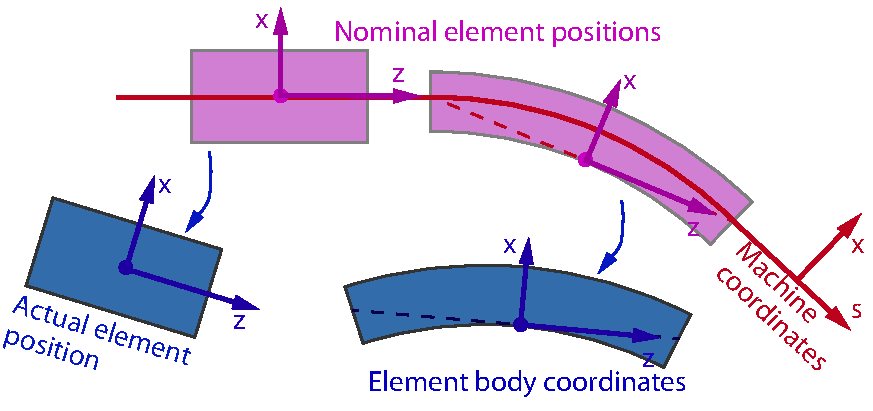
\includegraphics{alignment-ref.pdf} 
\caption[Element alignment.]  
{AlignmentGroup parameters The reference point is the origin
about which the element alignment is calculated. 
A) For straight elements, the reference point is in the center of the element. 
For \vn{Bend} elements, the reference point is at the midpoint of the chord connecting
the entrance point to the exit point. The drawing for the bend is valid for a \vn{ref_tilt}
of zero. For non-zero \vn{ref_tilt}, the outward direction from the bend center will not be
the $x$-axis. 
}  \label{f:alignment}
\end{figure}

\begin{figure}
\centering 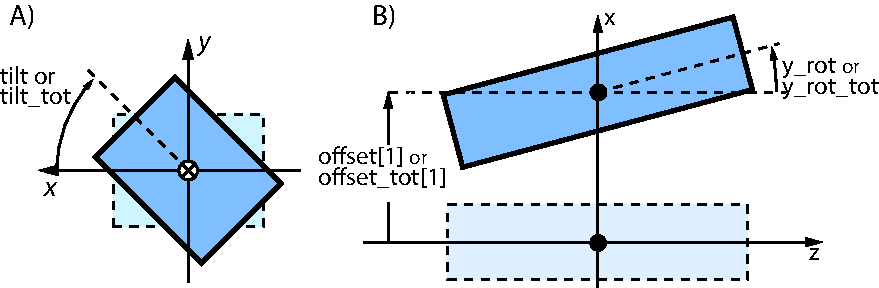
\includegraphics{alignment2.pdf} \caption[Alignment geometry.]  
{Alignment geometry. A) \vn{tilt} (or \vn{tilt_tot}) rotation. B) Combined
\vn{offset[1]} with \vn{y_rot} (or \vn{offset_tot[1]} with \vn{y_rot_tot}).
}  \label{f:alignment}
\end{figure}

The alignment group gives the alignment (position and angular orientation) of the physical element 
relative to the nominal position defined by the machine coordinates (\sref{s:orient}).
Alignment is specified with respect to the ``alignment reference point'' of an element as shown
in Fig~\ref{s:alignment}. The \vn{Bend} reference point is chosen to be the center of the chord
connecting the two ends. 
This reference point was chosen over using the midpoint on the reference orbit arc since a 
common simulation problem is to simulate a bend with a \vn{tilt} keeping the entrance and exit
endpoints fixed.

The parameters of the \vn{AlignmentGroup} can be divided into two sub-groups. 
One group has a \vn{_tot} suffix:
\begin{example}
  offset_tot::Vector - $[x, y, z]$ offset.
  x_rot_tot::Number  - Rotation around the x-axis.
  y_rot_tot::Number  - Rotation around the z-axis.
  tilt_tot::Number   - Rotation around the z-axis. 
\end{example}
These ``total alignment'' parameters give the alignment of the element with 
with respect to the machine coordinates.
The other sub-group of parameters do not have a \vn{_tot} suffix:
\begin{example}
  offset::Vector - $[x, y, z]$ offset.
  x_rot::Number  - Rotation around the x-axis.
  y_rot::Number  - Rotation around the z-axis.
  tilt::Number   - Rotation around the z-axis. 
\end{example}
These ``relative alignment'' parameters give the alignment of the element with respect 
to any \vn{Girder} that is supporting the element. 
If there is no support \vn{Girder}, the total alignment will be the same as the relative
alignment. The relative alignment can be set by the User. 
The total alignment is computed by \accellat based upon the relative alignment and the alignment
of any \vn{Girder}. \vn{Girder} elements themselves also have both relative and total
alignments since Girders can support other Girders.


%---------------------------------------------------------------------------------------------------
\section{ApertureGroup}
\label{s:aperture.g}


%---------------------------------------------------------------------------------------------------
\section{BMultipoleGroup}
\label{s:bmultipole.g}

%---------------------------------------------------------------------------------------------------
\section{BeamBeamGroup}
\label{s:beam.beam.g}

%---------------------------------------------------------------------------------------------------
\section{BendGroup}
\label{s:bend.g}

%---------------------------------------------------------------------------------------------------
\section{EMultipoleGroup}
\label{s:emulitipole.g}

%---------------------------------------------------------------------------------------------------
\section{FloorPositionGroup}
\label{s:floor.position.g}

%---------------------------------------------------------------------------------------------------
\section{GirderGroup}
\label{s:girder.g}

%---------------------------------------------------------------------------------------------------
\section{InitParticleGroup}
\label{s:init.particle.g}

%---------------------------------------------------------------------------------------------------
\section{LCavityGroup}
\label{s:lcavity.g}

%---------------------------------------------------------------------------------------------------
\section{LengthGroup}
\label{s:length.g}

%---------------------------------------------------------------------------------------------------
\section{LordSlaveGroup}
\label{s:lord.slave.g}

%---------------------------------------------------------------------------------------------------
\section{MasterGroup}
\label{s:master.g}

%---------------------------------------------------------------------------------------------------
\section{PatchGroup}
\label{s:patch.g}

%---------------------------------------------------------------------------------------------------
\section{RFFieldGroup}
\label{s:rffield.g}

%---------------------------------------------------------------------------------------------------
\section{RFGroup}
\label{s:rf.g}

%---------------------------------------------------------------------------------------------------
\section{RFMasterGroup}
\label{s:rfmaster.g}

%---------------------------------------------------------------------------------------------------
\section{ReferenceGroup}
\label{s:reference.g}

%---------------------------------------------------------------------------------------------------
\section{SolenoidGroup}
\label{s:solenoid.g}

%---------------------------------------------------------------------------------------------------
\section{StringGroup}
\label{s:string.g}

%---------------------------------------------------------------------------------------------------
\section{TrackingGroup}
\label{s:tracking.g}

%---------------------------------------------------------------------------------------------------
\section{TwissGroup}
\label{s:twiss.g}


\chapter{Constructing Lattices}
\label{c:construct-lat}

Note: 
\begin{example}
  @ele qq = Quadrupole()
  bl = beamline([.., qq, ..., qq, ...], ...)
\end{example}
Here changing parameters of qq will affect the parameters of the qq's in any beamline.
However, lattice expansion constructs the lattice with copies of qq so changing the
parameters of qq will not affect any of the copies in the lattice. This is done so that
parameters in the various qq's in the lattice are independent and an therefore differ from each
other. 

Branch geometry is inherited from the root line. To use a line with the "wrong" geometry, create
a new line using the old line with the "correct" geometry. EG
  ln2 = beamline(ln1.name, [ln1], geometry = CLOSED)
  lat = Lattice([ln2])

Note: OPEN and CLOSED are aliases for BranchGeometry.OPEN and BranchGeometry.CLOSED

* Show how to construct a Bmad replacement line using a function.

* Show how to get the effect of a Bmad List by replacing elements after expansion.

* Default name for end element is \vn{"endN"} where N is the index of the branch.
\chapter{Multipass}
\label{s:multipass}
\index{multipass|hyperbf}

%-----------------------------------------------------------------------------
\section{Multipass Fundamentals}
\label{s:multipass.fund}

\vn{Multipass} lines are a way to handle the bookkeeping when different elements being tracked
through represent the same physical element. For example, consider the case where dual ring colliding
beam machine is to be simulated. In this case the lattice file might look like:
\begin{example}
  ring1 = beamline("r1", [..., IR_region, ...])
  ring2 = beamline("r2", [..., reverse(IR_region), ...])
  IR_region = beamline("IR", [Q1, ....])
  lat = expand("dual_ring", [ring1, ring2])
\end{example}
[The \vn{reverse} construct means go through the line backwards (\sref{s:ele.reverse})] 
In this case, the \vn{Q1} element in \vn{ring1} and the
\vn{Q1} element in \vn{ring2} represent the same physical element.
Thus the parameters
of both the \vn{Q1}s should be varied in tandem. This can be done automatically using \vn{multipass}.
The use of multipass simplifies lattice and program development since the bookkeeping details are left
to the \accellat bookkeeping routines.

\index{multipass_slave}\index{multipass_lord}
To illustrate how \vn{multipass} works, consider the example of an Energy Recovery Linac (ERL) where
the beam will recirculate back through the LINAC section to recover the energy in the beam before it
is dumped. In \accellat, this situation can simulated by designating the LINAC section as \vn{multipass}.
The lattice file might look like:
\begin{example}
  @ele RF1 = LCavity(...)
  linac = beamline["linac", [RF1, ...], multipass = true)
  erl_line = beamline("erl", [linac, ..., linac])
  lat = expand("erl", [erl_line])
  rf1p2 = find_ele(lat, "RF1!mp1")
  rf1p2.multipass_phase = pi
\end{example}
The beamline called \vn{linac} is designated as \vn{multipass}. This \vn{linac} line appears twice in
the line \vn{erl_line} and \vn{erl_line} is the root line for lattice expansion. 
In branch 1 of the 
lattice, which will be a tracking branch, there will be two elements derived from the \vn{RF1} element:
\begin{example}
  RF1!mp1, ..., RF1!mp2, ...
\end{example}
Since the two elements are derived from a \vn{multipass} line, they are given unique names by adding
an \vn{!mpN} suffix where \vn{N} is an integer. 
These types of elements are known as \vn{multipass_slave} elements. In
addition to the \vn{multipass_slave} elements there will be a \vn{multipass_lord} element (that doesn't
get tracked through) called \vn{RF1} in the \vn{multipass_lord} branch of the lattice (\sref{s:lord.slave}).
Changes to the attributes of the lord \vn{RF1} element will be passed to the slave elements by the \accellat
bookkeeping routines. Assuming that the phase of \vn{RF1!mp1} gives acceleration, to make \vn{RF1!mp2}
decelerate, the \vn{multipass_phase} attribute of \vn{RF1!mp2} is set to pi. This is the one attribute
that \accellat's bookkeeping routines will not touch when transferring attribute values from \vn{RF1} to
its slaves. Notice that the \vn{multipass_phase} attribute had to be set after the lattice is formed
using the \vn{expand} function (\sref{s:expand}). This is true since 
\vn{RF1!mp2} does not exist before the lattice is expanded. \vn{multipass_phase} is useful with
relative time tracking \sref{s:rf.time}. However, \vn{multipass_phase} is ``unphysical'' and is just
a convenient way to shift the phase pass-to-pass through a given cavity. To ``correctly'' simulate
the recirculating beam, absolute time tracking should be used and the length of the lattice from a
cavity back to itself needs to be properly adjusted to get the desired phase advance. See the discussion
in section~\sref{s:rf.time}.

Multiple elements of the same name in a multipass line are considered 
physically distinct. Example:
\begin{example}
  m_line = beamline("m", [A, A, B], multipass = true)
  u_line = beamline("u", [m_line, m_line])
  lat = expand("lat", [u_line])
\end{example}
In this example, branch 1 of the lattice is:
\begin{example}
  A!mp1, A!mp1, B!mp1, A!mp2, A!mp2, B!mp2
\end{example}
In the \vn{multipass_lord} branch of the lattice there will be two multipass lords called \vn{A} and 
one another lord called \vn{B}. 
That is, there are three physically distinct elements in the lattice. The first
\vn{A} lord controls the 1\St and 4\Th elements in branch 1 and the second
\vn{A} lord controls the 2\Nd and 5\Th elements. If \vn{m_line} was {\em not} marked \vn{multipass},
branch 1 would have four \vn{A} and two \vn{B} elements and there would be
no lord elements.

Sublines contained in a multipass line that are themselves not marked multipass act the same as if
the elements of the subline where substituted directly in place of the subline in the containing
line. For example:
\begin{example}
  a_line = beamline("a", [A])
  m_line = beamline("m", [a_line, a_line], multipass = true)
  u_line = beamline("u", [m_line, m_line])
  lat = expand("lat", [u_line])
\end{example}
In this example, \vn{a_line}, which is a subline of the multipass \vn{m_line}, is {\em not}
designated \vn{multipass} and the result is the same as the previous example where \vn{m_line} was
defined to be \vn{(A, A, B)}. That is, there will be three physical elements represented by three
multipass lords.

Multipass lines do not have to be at the same ``level'' in terms of nesting of lines within
lines. Additionally, multipass can be used with line reversal (\sref{s:ele.reverse}). Example:
\begin{example}
  m_line = beamline("m", [A, B], multipass = true)
  m2_line = beamline("m2", m_line)
  @ele P = patch(...)  # Reflection patch
  u_line = beamline("u", [m_line, P, reverse(m2_line)])
  lat = expand("lat", [u_line])
\end{example}
Here the tracking part of the lattice is
\begin{example}
  A!mp1, B!mp1, ..., B!mp2 (r), A!mp2 (r)
\end{example}
The ``(r)'' here just denotes that the element is reversed and is not part of the name. The lattice
will have a multipass lord \vn{A} that controls the two \vn{A!mp n} elements and similarly with
\vn{B}. This lattice represents the case where, when tracking, 
a particle goes through the m_line in the ``forward''
direction and, at the reflection patch element \vn{P}, the coordinate system is reversed so that the particle
is then tracked in the reverse direction through the elements of \vn{m_line} twice.
While it is possible to use reflection ``$-$'' (\sref{s:lines.wo.arg}) instead
of reversal (\sref{s:ele.reverse}), reflection here does not make physical sense.  Needed
here is a reflection patch \vn{P} (\sref{s:patch}) between reversed and unreversed elements.

The procedure for how to group lattice elements into multipass slave groups which represent the same
physical element is as follows. For any given element in the lattice, this element has some line it
came from. Call this line $L_0$. The $L_0$ line in turn may have been contained in some other line
$L_1$, etc. The chain of lines $L_0$, $L_1$, ..., $L_n$ ends at some point and the last (top) line
$L_n$ will be one of the root lines listed in the \vn{use} statement (\sref{s:use}) in the lattice
file. For any given element in the lattice, starting with $L_0$ and proceeding upwards through the
chain, let $L_m$ be the {\em first} line in the chain that is marked as \vn{multipass}. If no such
line exists for a given element, that element will not be a multipass slave. For elements that have
an associated $L_m$ multipass line, all elements that have a common $L_m$ line and have the same
element index when $L_m$ is expanded are put into a multipass slave group (for a given line the
element index with respect to that line is 1 for the first element in the expanded line, the second
element has index 2, etc.).  For example, using the example above, the first element of the lattice,
\vn{A!mp1}, has the chain:
\begin{example}
    m_line, u_line
\end{example} 
The last element in the lattice, (\vn{A!mp2}), has the chain
\begin{example}
  m_line, m2_line, u_line
\end{example}
For both elements the $L_m$ line is \vn{m_line} and both elements are derived from the element with
index 1 with respect to \vn{m_line}. Therefore, the two elements will be slaved together.

As a final example, consider the case where a subline of a multipass line is also marked
\vn{multipass}:
\begin{example}
  a_line = beamline("a", [A], multipass = true)
  m_line = beamline("m", [a_line, a_line, B], multipass = true)
  u_line = beamline("u", [m_line, m_line])
  lat = expand("lat", [u_line])
\end{example}
In this case, branch 1 of the lattice will be:
\begin{example}
  A!mp1, A!mp2, B!mp1, A!mp3, A!mp4, B!mp2
\end{example}
There will be two lord elements representing the two physically distinct elements \vn{A} and \vn{B}.
The \vn{A} lord element will will control the four \vn{A!mpN} elements in the tracking
part of the lattice. The \vn{B} lord will control the two \vn{B!mpN} elements in the tracking part
of the lattice. 

To simplify the constructed lattice, if the set of lattice elements to slave together only contains
one element, a multipass lord is not constructed. For example:
\begin{example}
  m_line = beamline("m", [A, A, B], multipass = true)
  u_line = beamline([m_line])
  lat = expand("lat", [u_line])
\end{example}
In this example no multipass lords are constructed and the lattice is simply
\begin{example}
  A, A, B
\end{example}

It is important to note that the global coordinates (\sref{s:global}) of the slaves of a given
multipass lord are not constrained by \accellat to be the same. It is up to the lattice designer to make
sure that the physical positions of the slaves makes sense (that is, are the same).

%-----------------------------------------------------------------------------
\section{The Reference Energy in a Multipass Line}
\label{s:ref.e.multi}

Consider the lattice where the tracking elements are
\begin{example}
  A!mp1, C, A!mp2
\end{example}
where \vn{A!mp1} and \vn{A!mp2} are multipass slaves of element \vn{A} and \vn{C} is a \vn{lcavity}
element with some finite voltage. In this case, the reference energy calculation (\sref{s:energy})
where the reference energy of an element is inherited from the previous element, assigns differing
reference energies to \vn{A!mp1} and \vn{A!mp2}. In such a situation, what should be the assigned
reference energy for the multipass lord element \vn{A}? \accellat calculates the lord reference energy
in one of two ways. If, in the lattice file, \vn{e_tot_ref} or \vn{pc_ref} is set for the multipass lord
element, that setting will be used. If the reference energy (or reference momentum) is not set in the lattice
file, the reference energy of the lord is set equal to the reference energy of the first pass slave
element.

\chapter{Superposition}
\label{c:super}

%-----------------------------------------------------------------------------
\section{Superposition Fundamentals}
\label{s:super.fund}

In practice the field at a particular point in the lattice may be due to more than one physical
element. One example of this is a quadrupole magnet inside a larger solenoid magnet as shown in
\fig{f:super.ex}A. \bmad has a mechanism to handle this using what is called ``superposition''. A
simple example shows how this works (also see section \sref{s:lord.slave}):
\begin{example}
  using AcceleratorLattice
  @ele qq = Quadrupole(L = 4)
  @ele dd = Drift(L = 12)
  @ele ss = Solenoid(L = 1)
  @ele bb = BeginningEle(species_ref = species("proton"), pc_ref = 1e11)
  zline = beamline("z", [bb, qq, dd])
  lat = expand("lat", zline)
  dd_list = find_eles (lat, "dd")
  superimpose!(ss, dd_list, offset = 0.2)
\end{example}
The \vn{superimpose} attribute of element \vn{S} superimposes \vn{S} over the lattice \vn{(Q,
D)}. The placement of \vn{S} is such that the beginning of \vn{S} is coincident with the center of
\vn{Q} (this is is explained in more detail below). Additionally, a marker \vn{M} is superimposed at
a distance of +1~meter from the center of \vn{S}. The tracking part of the lattice
(\sref{s:lord.slave}) looks like:
\begin{example}
        Element   Key         Length  Total     
  1)    Q{\#}1       Quadrupole   2        2
  2)    Q{\B}S       Sol_quad     2        4
  3)    S{\#}1       Solenoid     3        7
  4)    M         Marker       0      
  4)    S{\#}2       Solenoid     3       10
  5)    D{\#}2       Drift        4       14
\end{example}
What \bmad has done is to split the original elements \vn{(Q, D)} at the edges of \vn{S} and then
\vn{S} was split where \vn{M} is inserted. The first element in the lattice, \vn{Q\#1}, is the part
of \vn{Q} that is outside of \vn{S}. Since this is only part of \vn{Q}, \bmad has put a \vn{\#1} in
the name so that there will be no confusion. (a single \vn{\#} has no special meaning other than the
fact that \bmad uses it for mangling names. This is opposed to a double \vn{\#\#} which is used to
denote the $N$\Th instance of an element (\sref{s:ele.match}). The next element, \vn{Q{\B}S}, is the
part of \vn{Q} that is inside \vn{S}. \vn{Q{\B}S} is a combination solenoid/quadrupole element as
one would expect. \vn{S{\#}1} is the part of \vn{S} that is outside \vn{Q} but before \vn{M}. This
element is just a solenoid. Next comes \vn{M}, \vn{S{\#}1}, and finally \vn{D\#2} is the rest of the
drift outside \vn{S}.

In the above example, \vn{Q} and \vn{S} will be \vn{super_lord} elements (\vn{s:lord.slave}) and
four elements in the tracking part of the lattice will be \vn{super_slave} elements. This is
illustrated in \fig{f:super.ex}B.

Notice that the name chosen for the \vn{sol_quad} element \vn{Q{\B}S} is dependent upon what is
being superimposed upon what. If \vn{Q} had been superimposed upon \vn{S} then the name would have
been \vn{S{\B}Q}.

When \bmad sets the element class for elements created from superpositions, \bmad will set the class
of the element to something other than an \vn{em_field} element (\sref{s:em.field}) if possible. If
no other possibilities exist, \bmad will use \vn{em_field}. For example, a \vn{quadrupole}
superimposed with a \vn{solenoid} will produce a \vn{sol_quad} \vn{super_slave} element but a
\vn{solenoid} superimposed with a \vn{rfcavity} element will produce an \vn{em_field} element since
there is no other class of element that can simultaneously handle solenoid and RF fields. An
\vn{em_field} \vn{super_slave} element will also be created if any of the superimposing elements 
have a non-zero orientation (\sref{s:offset}) since it is not, in general, possible to construct a slave
element that properly mimics the effect of a non-zero orientation.

  \begin{figure}[tb]
  \centering 
  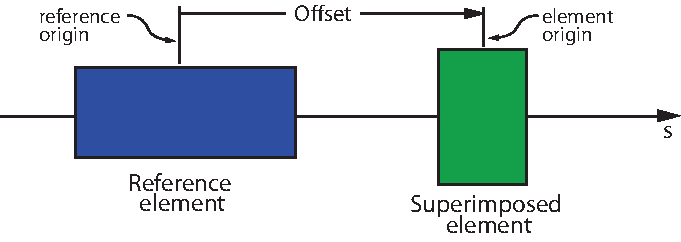
\includegraphics[width=0.8\textwidth]{superimpose-positioning.pdf} 
  \caption[Superposition Offset.]{
The superposition offset is the longitudinal $s$-distance from the origin point of the
reference element to the origin point of the element being superimposed.
  }
  \label{f:superimpose}
  \end{figure}

With the lattice broken up like this \bmad has constructed something that can be easily
analyzed. However, the original elements \vn{Q} and \vn{S} still exist within the lord section of
the lattice. \bmad has bookkeeping routines so that if a change is made to the \vn{Q} or \vn{S}
elements then these changes can get propagated to the corresponding slaves. It does not matter which
element is superimposed. Thus, in the above example, \vn{S} could have been put in the Beam Line
(with a drift before it) and \vn{Q} could then have been superimposed on top and the result would
have been the same (except that the split elements could have different names).

If an element has zero length (for example, a \vn{marker} element), is superimposed, or is
superimposed upon, then the element will remain in the tracking part of the lattice and there will
be no corresponding lord element. See \fig{f:super.ex}.
 
Superimpose syntax:
\begin{example}
  Q: quad, superimpose, ...       ! Superimpose element Q.
  Q: quad, superimpose = T, ...   ! Same as above.
  Q: quad, ...                    ! First define element Q ...
  Q[superimpose] = T              !   ... and then superimpose.
  Q[superimpose] = F              ! Suppress superposition.
\end{example}
Superposition happens at the end of parsing so the last set of the \vn{superimpose} for an element
will override previous settings. 

It is also possible to superimpose an element using the \vn{superimpose} command which has the
syntax:
\begin{example}
  superimpose, element = <ele-name>, ...
\end{example}
With the same optional superposition parameters (\vn{ref}, \vn{offset}, etc.) given below.
Example:
\begin{example}
  superimpose, element = Q1, ref = B12, offset = 1.3, 
                               ele_origin = beginning, ref_origin = end
\end{example}
Note: Superposition using the superimpose statement allows superimposing the same element with
multiple reference elements and/or multiple offsets. The drawback is that superposition using the
superimpose statement may not be switched off later in the lattice file.

The placement of a superimposed element is illustrated in \fig{f:superimpose}. The placement of a
superimposed element is determined by three factors: An origin point on the superimposed element, an
origin point on the reference element, and an offset between the points. The attributes that
determine these three quantities are:
\index{ref}\index{offset}
\index{ref_origin}\index{ele_origin}
\begin{example}
  create_jumbo_slave = <Logical>     ! See \sref{s:jumbo.slave}
  wrap_superimpose   = <Logical>     ! Wrap if element extends past lattice ends?
  ref          = <lattice_element>
  offset       = <length>            ! default = 0
  ele_origin   = <origin_location>   ! Origin pt on element.
  ref_origin   = <origin_location>   ! Origin pt on ref element.
\end{example}
\vn{ref} sets the reference element. If \vn{ref} is not present then the start of the lattice is
used (more precisely, the start of branch 0 (\sref{s:branch.def})). Wild card characters
(\sref{s:ele.match} can be used with \vn{ref}. If \vn{ref} matches to multiple elements (which may
also happen without wild card characters if there are multiple elements with the name given by
\vn{ref}) in the lattice a superposition will be done, one for each match.

The location of the origin points are determined by the setting of \vn{ele_origin} and
\vn{ref_origin}.  The possible settings for these parameters are
\begin{example}
  beginning       ! Beginning (upstream) edge of element
  center          ! Center of element. Default.
  end             ! End (downstream) edge of element
\end{example}
\vn{center} is the default setting. \vn{Offset} is the longitudinal offset of the origin 
of the element being superimposed relative
to the origin of the reference element. The default offset is zero.  
A positive offset moves the element being superimposed in the \vn{downstream} direction if
the reference element has a normal longitudinal \vn{orientation} (\sref{s:ele.reverse}) and
vice versa for the reference element has a reversed longitudinal orientation.

Note: There is an old syntax, deprecated but still supported for now, where the origin points were
specified by the appearance of:
\begin{example}
  ele_beginning         ! Old syntax. Do not use.
  ele_center            ! Old syntax. Do not use.
  ele_end               ! Old syntax. Do not use.
  ref_beginning         ! Old syntax. Do not use.
  ref_center            ! Old syntax. Do not use.
  ref_end               ! Old syntax. Do not use.
\end{example}
For example, ``ele_origin = beginning'' in the old syntax would be ``ele_beginning''.

\index{drift}
\index{overlay}\index{group}\index{girder}
The element begin superimposed may be any type of element except \vn{drift}, \vn{group},
\vn{overlay}, and \vn{girder} control elements. The reference element used to position a
superimposed element may be a \vn{group} or \vn{overlay} element as long as the \vn{group} or
\vn{overlay} controls the attributes of exactly one element. In this case, the controlled element is
used as the reference element.

\index{geometry}\index{open}
By default, a superimposed element that extends beyond either end of the lattice will be wrapped
around so part of the element will be at the beginning of the lattice and part of the element will
be at the end. For consistency's sake, this is done even if the \vn{geometry} is set to \vn{open}
(for example, it is sometimes convenient to treat a circular lattice as linear). Example:
\begin{example}
  d: drift, l = 10
  q: quad, l = 4, superimpose, offset = 1
  machine: line = (d)
  use, machine
\end{example}
The lattice will have five elements in the tracking section:
\begin{example}
        Element    Key             Length
  0)    BEGINNING  Beginning_ele   0
  1)    Q{\#}2        Quadrupole      3   ! Slave representing beginning of Q element
  2)    D{\#}1        Drift           6
  3)    Q{\#}1        Quadrupole      1   ! Slave representing end of Q element
  4)    END        Marker          0
\end{example}
And the lord section of the lattice will have the element \vn{Q}. 

To not wrap an element that is being superimposed, set the \vn{wrap_superimpose} logical to \vn{False}.
Following the above example, if the definition of\vn{q} is extended by adding \vn{wrap_superimpose}:
\begin{example}
  q: quad, l = 4, superimpose, offset = 1, wrap_superimpose = F
\end{example}
In this instance there are four elements in the tracking section:
\begin{example}
        Element    Key             Length
  0)    BEGINNING  Beginning_ele   0
  1)    Q          Quadrupole      4    
  2)    D{\#}1        Drift           7
  4)    END        Marker          0
\end{example}
And the lord section of the lattice will not have any elements.

To superimpose a zero length element ``\vn{S}'' next to a zero length element ``\vn{Z}'', and to
make sure that \vn{S} will be on the correct side of \vn{Z}, set the \vn{ref_origin} appropriately.
For example:
\begin{example}
  S1: marker, superimpose, ref = Z, ref_origin = beginning
  S2: marker, superimpose, ref = Z, ref_origin = end
  Z: marker
\end{example}
The order of the elements in the lattice will be
\begin{example}
  S1, Z, S2
\end{example}
If \vn{ref_origin} is not present or set to \vn{center}, the ordering of the elements will be
arbitrary.

If a zero length element is being superimposed at a spot where there are other zero length elements,
the general rule is that the element will be placed as close as possible to the reference element.
For example:
\begin{example}
  S1: marker, superimpose, offset = 1
  S2: marker, superimpose, offset = 1
\end{example}
In this case, after \vn{S1} is superimposed at $s = 1$ meter, the superposition of \vn{S2} will
place it as close to the reference element, which in this case is the \vn{BEGINNING} elements at $s
= 0$, as possible. Thus the final order of the superimposed elements is:
\begin{example}
  S2, S1
\end{example}
To switch the order while still superimposing \vn{S2} second one possibility is to use:
\begin{example}
  S1: marker, superimpose, offset = 1
  S2: marker, superimpose, ref = S1, ref_origin = end
\end{example}

If a superposition uses a reference element, and there are $N$ elements in the lattice with the
reference element name, there will be $N$ superpositions. For example, the following will split in
two all the quadrupoles in a lattice:
\begin{example}
  M: null_ele, superimpose, ref = quadrupole::*
\end{example}
A \vn{null_ele} (\sref{s:null.ele}) element is used here so that there is no intervening element
between split quadrupole halves as there would be if a \vn{marker} element was used.


\index{drift!superposition}\index{pipe!superposition}
When a superposition is made that overlaps a drift, the drift, not being a "real" element,
vanishes. That is, it does not get put in the lord section of the lattice.  Note that if aperture
limits (\sref{s:limit}) have been assigned to a drift, the aperture limits can ``disappear'' when
the superposition is done. Explicitly, if the exit end of a drift has been assigned aperture limits,
the limits will disappear if the superimposed element overlays the exit end of the drift. A similar
situation applies to the entrance end of a drift. If this is not desired, use a \vn{pipe} element
instead. 

To simplify bookkeeping, a drift element may not be superimposed. Additionally, since drifts can
disappear during superposition, to avoid unexpected behavior the superposition reference element may
not be the $N$\Th instance of a drift with a given name. For example, if there are a number of drift
elements in the lattice named \vn{a_drft}, the following is not allowed:
\begin{example}
  my_oct: octupole, ..., superimpose, ref = a_drft##2  ! This is an error
\end{example}

When the attributes of a super_slave are computed from the attributes of its super_lords, some types
of attributes may be ``missing''. For example, it is, in general, not possible to set appropriate
aperture attributes (\sref{s:limit}) of a super_slave if the lords of the slave have differing
aperture settings. When doing calculations, \bmad will use the corresponding attributes stored in
the lord elements to correctly calculate things.

When superposition is done in a line where there is \vn{element reversal} (\sref{s:ele.reverse}),
the calculation of the placement of a superimposed element is also ``reversed'' to make the relative
placement of elements independent of any element reversal.  An example will make this clear:
\begin{example}
  d1: drift, l = 1
  d2: d1
  q1: quad, l = 0.1, superimpose, ref = d1, offset = 0.2, 
             ref_origin = beginning, ele_origin = beginning
  q2: q1, ref = d2
  p: patch, x_pitch = pi  ! Needed to separate reversed and unreversed.
  this_line: line = (d1, p, --d2)
  use, this_line
\end{example}
Since the reference element of the \vn{q2} superposition, that is \vn{d2}, is a reversed element,
\vn{q2} will be reversed and the sense of \vn{offset}, \vn{ref_origin}, and \vn{ele_origin} will be
reversed so that the position of \vn{q2} with respect to \vn{d2} will be the mirror image of the
position of \vn{q1} with respect to \vn{d1}. The tracking part of the lattice will be:
\begin{example}
  Element:           d1{\#}1    q1  d1{\#}2   d2{\#}2    q2   d2{\#}1
  Length:             0.2   0.1   0.7    0.7   0.1    0.3
  Reversed element?:   No    No    No    Yes   Yes    Yes
\end{example}

Superposition with \vn{line reflection} (\sref{s:lines.wo.arg}) works the same way as line reversal.

The \vn{no_superposition} statement (\sref{s:no.sup}) can be used to turn off superpositioning

%-----------------------------------------------------------------------------
\section{Superposition and Sub-Lines}
\label{s:super.sub.line}

Sometimes it is convenient to do simulations with only part of a lattice. The rule for how
superpositions are handled in this case is illustrated in the following example. Consider a lattice
file which defines a \vn{line} called \vn{full} which is defined by two sublines called \vn{sub1}
and \vn{sub2}:
\begin{example}
  sub1: line = {..., ele1, ...}
  sub2: line = {...}
  full: line = {sub1, sub2}
  m1: marker, superimpose, ref = ele1, offset = 3.7
  use, full
\end{example}
Now suppose you want to do a simulation using only the \vn{sub2} line. Rather than edit the original
file, one way to do this would be to create a second file which overrides the used line:
\begin{example}
  call, file = "full.bmad"
  use, sub2
\end{example}
where \vn{full.bmad} is the name of the original file. What happens to the superposition of \vn{m1}
in this case? Since \vn{m1} uses a reference element, \vn{ele1}, that is not in \vn{sub1}, \bmad
will ignore the superposition. Even though \bmad will ignore the superposition of \vn{m1} here,
\bmad will check that \vn{ele1} has been defined. If \vn{ele1} has not been defined, \bmad will
assume that there is a typographic error and issue an error message.

Notice that in this case it is important for the superposition to have an explicit reference element
since without an explicit reference element the superposition is referenced to the beginning of the
lattice. Thus, in the above example, if the superposition were written like:
\begin{example}
  m1: marker, superimpose, offset = 11.3
\end{example}
then when the \vn{full} line is used, the superposition of \vn{m1} is referenced to the beginning of
\vn{full} (which is the same as the beginning of \vn{sub1}) but when the \vn{sub2} line is used, the
superposition of \vn{m1} is referenced to the beginning of \vn{sub2} which is not the same as the
beginning of \vn{full}.

%-----------------------------------------------------------------------------
\section{Jumbo Super_Slaves}
\label{s:jumbo.slave}

The problem with the way \vn{super_slave} elements are created as discussed above is that edge
effects will not be dealt with properly when elements with non-zero fields are misaligned. When this
is important, especially at low energy, a possible remedy is to instruct \bmad to construct
``\vn{jumbo}'' super_slave elements. The general idea is to create one large \vn{super_slave} for
any set of overlapping elements. Returning to the superposition example at the start of
Section~\sref{s:super}, If the superposition of solenoid \vn{S} is modified to be
\begin{example}
  S: solenoid, l = 8, superimpose, ref = Q, ele_origin = beginning, 
               create_jumbo_slave = T
\end{example}
The result is shown in \fig{f:super.ex}C. The tracking part of the lattice will be
\begin{example}
        Element   Key         Length  Total     
  1)    Q{\B}S       Sol_quad     2        4
  2)    M         Marker       0      
  3)    S{\#}2       Solenoid     3       10
  4)    D{\#}2       Drift        4       14
\end{example}
\index{lord_pad1}\index{lord_pad2}
\vn{Q} and part of \vn{S} have been combined into a jumbo \vn{super_slave} named \vn{Q{\B}S}. Since
the \vn{super_lord} elements of a jumbo \vn{super_slave} may not completely span the slave two
attributes of each lord will be set to show the position of the lord within the slave. These two
attributes are
\begin{example}
  lord_pad1    ! offset at upstream end
  lord_pad2    ! offset at downstream end
\end{example}
\vn{lord_pad1} is the distance between the upstream edge of the jumbo \vn{super_slave} and a
\vn{super_lord}. \vn{lord_pad2} is the distance between the downstream edge of a \vn{super_lord} and
the downstream edge of the jumbo \vn{super_slave}. With the present example, the lords have the
following padding:
\begin{example}
          lord_pad1    lord_pad2
  Q            0            3
  S            2            0
\end{example}
The following rule holds for all super lords with and without jumbo slaves:
\begin{example}
  Sum of all slave lengths = lord length + lord_pad1 + lord_pad2
\end{example}

One major drawback of jumbo \vn{super_slave} elements is that the \vn{tracking_method}
(\sref{s:tkm}) will, by necessity, have to be \vn{runge_kutta}, or \vn{time_runge_kutta} and the
\vn{mat6_calc_method} (\sref{s:xfer}) will be set to \vn{tracking}.

Notice that the problem with edge effects for non-jumbo \vn{super_slave} elements only occurs when
elements with nonzero fields are superimposed on top of one another. Thus, for example, one does not
need to use jumbo elements when superimposing a \vn{marker} element.

\index{field_overlaps}
Another possible way to handle overlapping fields is to use the \vn{field_overlaps} element
attribute as discussed in \sref{s:overlap}.

%-----------------------------------------------------------------------------
\section{Changing Element Lengths when there is Superposition}
\label{s:super.length}

When a program is running, if \vn{group} (\sref{s:group}) or \vn{overlay} (\sref{s:overlay})
elements are used to vary the length of elements that are involved in superimposition, the results
are different from what would have resulted if instead the lengths of the elements where changed in
the lattice file. There are two reasons for this. First, once the lattice file has been parsed,
lattices can be ``mangled'' by adding or removing elements in a myriad of ways. This means that it
is not possible to devise a general algorithm for adjusting superimposed element lengths that
mirrors what the effect of changing the lengths in the lattice file.

Second, even if a lattice has not been mangled, an algorithm for varying lengths that is based on
the superimpose information in the lattice file could lead to unexpected results. To see this
consider the first example in Section~\sref{s:super}. If the length of \vn{S} is varied in the
lattice file, the upstream edge of \vn{S} will remain fixed at the center of \vn{Q} which means that
the length of the \vn{super_slave} element \vn{Q{\#}1} will be invariant. On the other hand, if
element \vn{S} is defined by
\begin{example}
  S: solenoid, l = 8, superimpose, offset = 6
\end{example}
This new definition of \vn{S} produces exactly the same lattice as before. However, now varying the
length of \vn{S} will result in the center of \vn{S} remaining fixed and the length of \vn{Q{\#}1}
will not be invariant with changes of the length of \vn{S}. This variation in behavior could be very
confusing since, while running a program, one could not tell by inspection of the element positions
what should happen if a length were changed.

To avoid confusion, \bmad uses a simple algorithm for varying the lengths of elements involved in
superposition: The rule is that the length of the most downstream \vn{super_slave} is varied.  With
the first example in Section~\sref{s:super}, the \vn{group} \vn{G} varying the length of \vn{Q}
defined by:
\begin{example}
  G: group = \{Q\}, var = \{l\}
\end{example}
would vary the length of \vn{Q{\B}S} which would result in an equal variation of the length of
\vn{S}. To keep the length of \vn{S} invariant while varying \vn{Q} the individual \vn{super_slave}
lengths can be varied. Example:
\begin{example}
  G2: group = \{Q{\#}1, S{\#}1:-1\}, var = \{l\}
\end{example}
The definition of \vn{G2} must be placed in the lattice file after the superpositions so that the
super slaves referred to by \vn{G2} have been created.

In the above example there is another, cleaner, way of achieving the same result by varying the
downstream edge of \vn{Q}:
\begin{example}
  G3: group = \{Q\}, var = \{end_edge\}
\end{example}

\etcetc...

*) Difference from Bmad: Superposition is always done after lattice expansion.

*) Superimposing on a given drift multiple times is not allowed (unlike Bmad). 
  Instead, superimpose a Null ele at the beginning or end of the drift.


\chapter{Customizing Lattices}
\label{c:custom-lat}


%---------------------------------------------------------------------------------------------------
\vn{Custom Lattice Element Parameters}

Custom parameters may be added to lattice elements but methods need to be created to tell \accellat
how to handle these parameters.

* Define element parameter group

* Need to extend:
  ele_param_info_dict
  ele_param_groups


%---------------------------------------------------------------------------------------------------
\vn{Custom Lattice Elements}

* Need to extend:
  ele_param_groups


\chapter{Utilities}
\label{c:utilities}

This chapter covers utility functions.

%---------------------------------------------------------------------------------------------------
\section{Iteration Over Elements in a Lattice}
\label{s:iteration}

Iteration over a Region (see traversal.jl)

%---------------------------------------------------------------------------------------------------
\section{Searching for Lattice Elements}
\label{s:search}

%---------------------------------------------------------------------------------------------------
\section{Particle Properties Conversion Functions}
\label{s:conversion}

%---------------------------------------------------------------------------------------------------
\section{Math Utilities}
\label{s:math}

%---------------------------------------------------------------------------------------------------
\section{Lattice Manipulation}
\label{s:manipulation}

%---------------------------------------------------------------------------------------------------
\section{Miscellaneous Utilities}
\label{s:misc.utilities}


%---------------------------------------------------------------------------------------------------
\part{Conventions and Physics}
%---------------------------------------------------------------------------------------------------

\chapter{Coordinates}
\label{s:coords}
\index{coordinates|hyperbf}

\vspace*{-0.3in}
\bmad uses three coordinate systems as illustrated in \fig{f:coords}. First, the \vn{global} (also
called ``\vn{floor}'') coordinates are independent of the placement accelerator. Things such as the
building the accelerator is in may be described using \vn{global} coordinates.

\begin{figure}[!b]
  \centering
  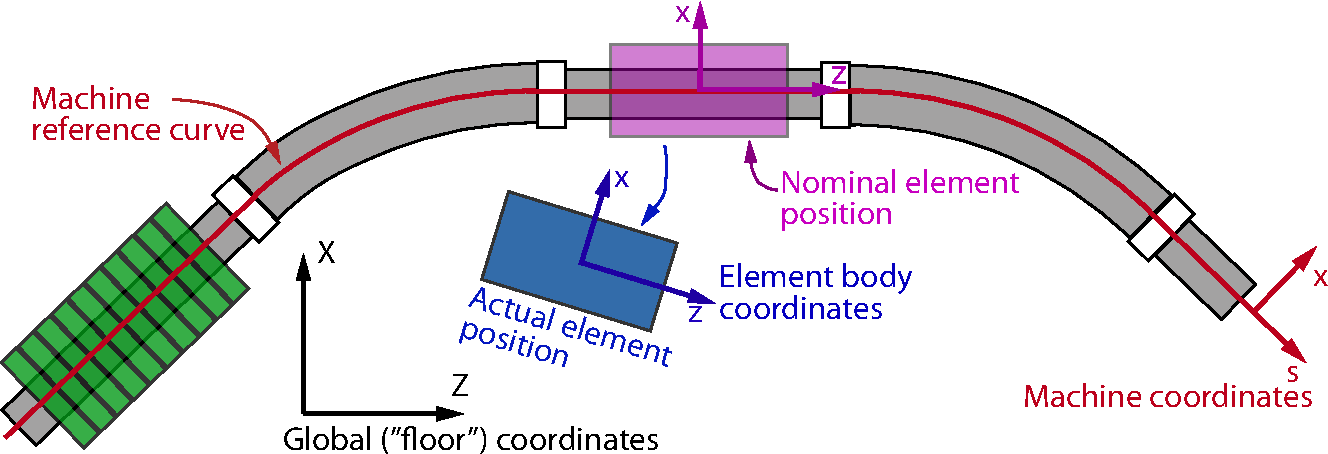
\includegraphics[width=5.0in]{coordinates.pdf}
  \caption[The three coordinate system used by \bmad.]
{The \vn{global} (or ``\vn{floor}'') coordinate system
is independent of the accelerator.  The \vn{machine} curvilinear coordinate system follows the bends
of the accelerator.  Each lattice element has \vn{element body} coordinates which, if the element is
not ``misaligned'' is the same as the \vn{machine} coordinates. 
The $x=y=0$ curved line of the
machine coordinate system is known as the ``reference orbit''.}
  \label{f:coords}
\end{figure}

It is inconvenient to describe the position of a particle beam using the 
\vn{global} coordinate system so
a ``\vn{machine}'' coordinate system is used (\sref{s:machine.coords}).  This curvilinear coordinate
system defines the nominal position of the lattice elements.  The relationship between the
\vn{machine} and \vn{global} coordinate systems is described in \sref{s:global}.

The ``nominal'' position of a lattice element is the position of the element without any
position and orientation shifts (\sref{s:align.g}) 
which are sometimes referred to as ``misalignments''. 
Each lattice element has ``\vn{element body}'' (or just ``\vn{body}'') 
coordinates which are attached to the physical element and the electric and magnetic
fields of an element are described with respect to \vn{body} coordinates.  If there are no
misalignments, the \vn{body} coordinates are aligned with the 
\vn{machine} coordinates.
The transformation between \vn{machine} and \vn{body} coordinates is given in
\sref{s:lab.body.transform}.
The $x=y=0$ curved line of the
machine coordinate system is known as the ``\vn{reference orbit}''.

%-----------------------------------------------------------------------------
\section{Machine Coordinates and Reference Orbit}
\label{s:machine.coords}

%-----------------------------------------------------------------------------
\subsection{The Reference Orbit}
\label{s:ref}
\index{reference orbit|hyperbf}
\index{machine coordinates|hyperbf}

\begin{figure}[tb]
  \centering
  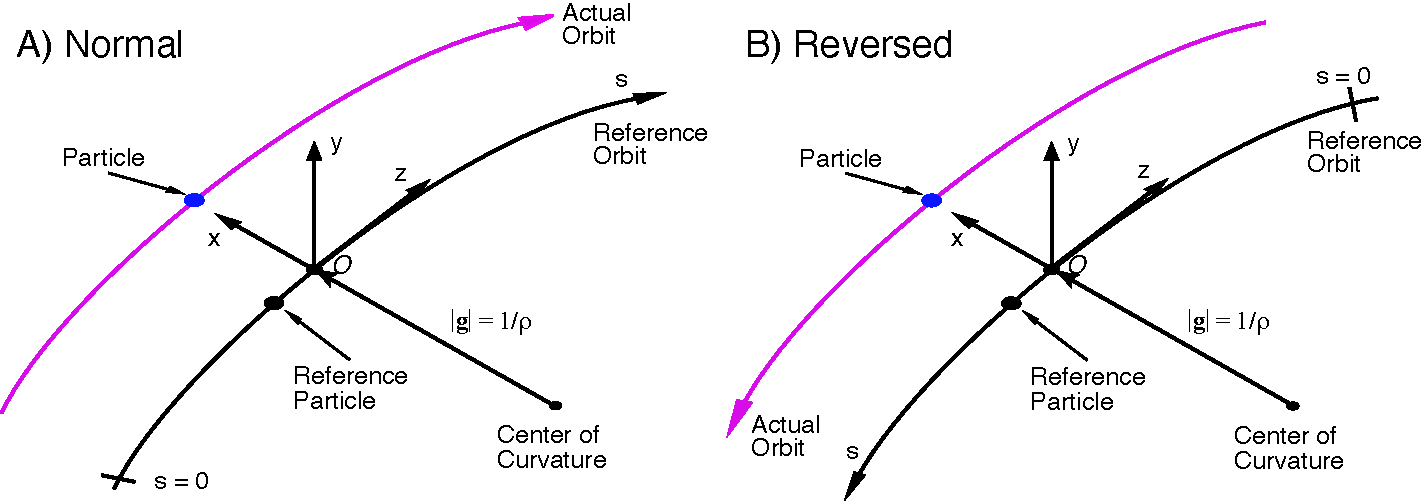
\includegraphics[width=6in]{machine-coords.pdf}
  \caption[Reference coordinate system.]
{The reference coordinate system. By construction, a particle's $z$ coordinate is zero.  This
is not to be confused with the phase space $z$ coordinate (\sref{s:phase.space}). The curvature
vector $\bfg$ lies in the $x$-$y$ plane and has a magnitude of $1/\rho$ where $\rho$ is the bending
radius. A) The $z$-axis will normally be parallel to the $s$-axis. B) For \vn{reversed} elements it
will be antiparallel. In both cases, the particle and reference particle are traveling in the
direction of greater $s$.}
  \label{f:machine.coords}
\end{figure}

The \vn{machine reference orbit} is the curved path used to define a coordinate system for describing
a particle's position as shown in \fig{f:machine.coords}. The reference orbit is also used for
orientating lattice elements in space. At a given time $t$, a particle's position can be described
by a point $\calO$ on the reference orbit a distance $s$ relative to the reference orbit's zero
position plus a transverse $(x,y)$ offset. The point $\calO$ on the reference orbit is used as the
origin of the machine $(x, y, z)$ coordinate system with the $z$--axis tangent to the reference
orbit. The $z$--axis will generally be pointing in the direction of increasing $s$
(\fig{f:machine.coords}A) but, as discussed below, will point counter to $s$ for elements that are
longitudinally \vn{reversed} in orientation (\fig{f:machine.coords}B). 
The $x$ and $y$--axes are perpendicular to the reference
orbit and, by construction, the particle is always at $z = 0$. The coordinate system so constructed
is called the \vn{``machine coordinate system''} when there is need to distinguish it from the 
\vn{``element body coordinate system''}
(\sref{s:coords}) which is attached to the physical element. There is a separate reference orbit
for each branch (\sref{s:branch.def}) of a lattice.

\index{x_offset}\index{y_offset}
\index{x_rot}\index{y_rot}\index{wiggler}
The reference orbit may not correspond to the orbit that any actual particle could travel.
A common example is the \vn{wiggler} element where particles always oscillate about the reference
orbit which is a straight line.

Do not confuse this reference orbit (which defines the machine coordinate system) with the reference
orbit about which the transfer maps are calculated (\sref{s:twiss}). The former is fixed by the
lattice while the latter can be any arbitrary orbit.

%-----------------------------------------------------------------------------
\subsection{Element Entrance and Exit Coordinates}
\label{s:ent.exi}
\index{element body coordinates}

%--------------------------------------

  \begin{figure}[tb]
  \centering
  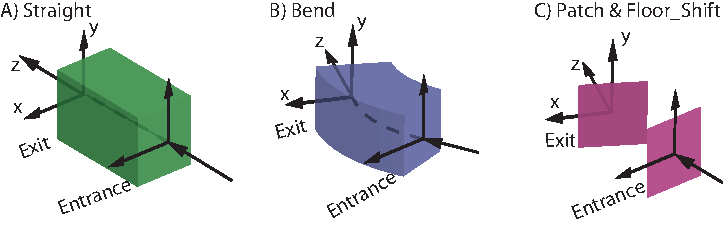
\includegraphics[width=5in]{ele-coord-frame.pdf}
\caption[Lattice elements as LEGO blocks.]{Lattice elements can be imagined as ``LEGO blocks'' which
fit together to form the reference orbit along with the machine coordinate system. How elements
join together is determined in part by their entrance and exit coordinate frames. A) For
straight line elements the entrance and exit frames are colinear. B) For bends elements, the two
frames are rotated with respect to each other. C) For \vn{patch} and \vn{floor_shift} elements the
exit frame may be arbitrarily positioned with respect to the entrance frame.}
  \label{f:ele.coord.frame}
  \end{figure}

%--------------------------------------

\index{sbend}\index{rbend}
\index{crystal}\index{mirror}\index{entrance_end}
\index{exit_end}\index{patch}\index{floor_shift}
One way of thinking about the reference orbit and machine coordinates is to imagine that each
element is like a LEGO block with an ``\vn{entrance}'' and an ``\vn{exit}'' coordinate frame as
illustrated in \fig{f:ele.coord.frame}\footnote
  {
Thanks to Dan Abell for this analogy.
  }. 
These coordinate frames are attached to the element. that is, things like electric and magnetic
fields, apertures, etc., are described with respect to the entrance and exit coordinates.  Thus, for
example, the \vn{e1} edge of a \vn{Bend} (\sref{s:bend}) is always at the \vn{entrance} face and the
\vn{e2} is always at the \vn{exit} face. Most elements have a ``straight'' geometry as shown in
\fig{f:ele.coord.frame}A. That is, the reference orbit through the element is a straight line
segment with the $x$ and $y$ axes always pointing in the same direction.  For a \vn{Bend} element
(\sref{s:bend}), the reference orbit is a segment of a circular arc as shown in
\fig{f:ele.coord.frame}B. With the \vn{ref_tilt} parameter of a bend set to zero, the rotation axis
between the entrance and exit frames is parallel to the $y$-axis (\sref{s:global}). For \vn{Patch}
(\sref{s:patch}), and \vn{floor_shift} (\sref{s:floorshift}) elements, the exit face can can
arbitrarily oriented with respect to the entrance end. For the \vn{FloorShift} element the
interior reference orbit between the
entrance and exit faces is not defined. For the \vn{Patch} element, the interior reference orbit 
is dependent upon certain \vn{Patch} element parameter settings.

%-----------------------------------------------------------------------------
\subsection{Reference Orbit and Machine Coordinates Construction}
\label{s:ref.construct}
\index{reference orbit!construction}
\index{upstream element end}\index{downstream element end}
\index{entrance element end}\index{exit element end}

%-----------------------------------------------------------------------------
\begin{figure}[tb]
  \centering
  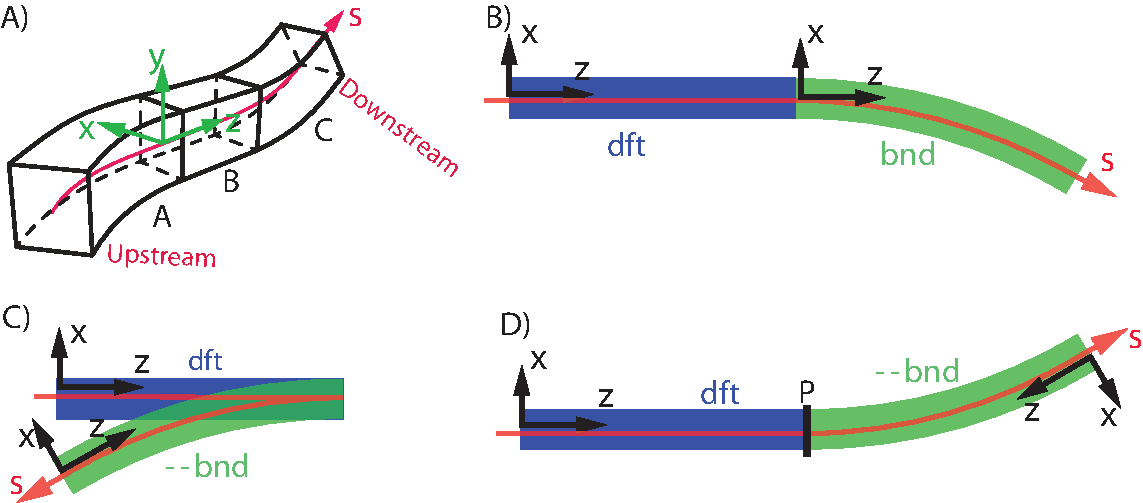
\includegraphics[width=5in]{patch-between.pdf}
  \caption[Machine coordinates construction.]{A) The machine coordinates are constructed by
connecting the \vn{downstream} reference frame of one element with the \vn{upstream} reference frame
of the next element in the branch. Coordinates shown is for the mating of element \vn{A} to element
{B}.  B) Example with drift element \vn{dft} followed by a bend \vn{bnd}. Both elements are
unreversed. C) Similar to (B) but in this case element \vn{bnd} is reversed.  D) Similar to (C) but
in this case a reflection patch has been added in between \vn{dft} and \vn{bnd}.  In (B), (C), and
(D) the $(x,z)$ coordinates are drawn at the \vn{entrance} end of the elements. The $y$ coordinate
is always out of the page.}
  \label{f:patch.between}
\end{figure}
%-----------------------------------------------------------------------------

\index{root branch}
Assuming for the moment that there are no \vn{fiducial} elements present, the construction of the
reference orbit starts at the \vn{BeginningEle} element (\sref{s:begin.ele}) at the start of a
branch. If the branch is a \vn{root} branch (\sref{s:lattice.def}), The orientation of the beginning
element within the global coordinate system (\sref{s:coords}) can be fixed by setting 
FloorPositionGroup parameters (\sref{floor.g}
positioning statements (\sref{s:beginning}). If the branch is not a \vn{root} branch, the position
of the beginning element is determined by the position of the \vn{fork} or \vn{photon_fork} element
from which the branch forks from. Unless set otherwise in the lattice file, $s = 0$ at the
\vn{BeginningEle} element.

If there are \vn{fiducial} elements, the machine coordinates are constructed beginning at these
elements.

Once the beginning element in a branch is positioned, succeeding elements are concatenated together
to form the machine coordinates. All elements have an ``\vn{upstream}'' and a ``\vn{downstream}''
end as shown in \fig{f:patch.between}A. The \vn{downstream} end of an element is always farther (at
greater $s$) from the beginning element than the \vn{upstream} end of the element.  Particles travel
in the $+s$ direction, so particles will enter an element at the upstream end and exit at the
downstream end.

Normally, the \vn{upstream} end is the same as the element's \vn{entrance} end 
(\fig{f:ele.coord.frame}) and the
\vn{downstream} end is the same as the element's \vn{exit} end. However, if an element is reversed
(\sref{s:ele.reverse}), the element's \vn{exit} end will be \vn{upstream} end and the element's
\vn{entrance} end will be the \vn{downstream} end. That is, for a reversed element, particles 
traveling downstream will
enter at the element's \vn{exit} end and will exit at the \vn{entrance} end.

The procedure to connect elements together to form the machine coordinates is to mate the
downstream reference frame of the element with the upstream reference frame of the next element in
the branch so that, without misalignments, the $(x,y,z)$ axes coincide\footnote
  {
If there are misalignments, the \vn{entrance} and \vn{exit} frames will move with the element. However,
the \vn{upstream} and \vn{downstream} frames, along with the reference orbit and machine
coordinates, will not move.
  }. 
This is illustrated in \fig{f:patch.between}. \fig{f:patch.between}A shows the general situation
with the downstream frame of element \vn{A} mated to the upstream frame of element \vn{B}.
Figures~\ref{f:patch.between}B-C show branches constructed from the following lattice file:
\begin{example}
  @ele dft = drift(L = 2)
  @ele bnd = bend(l = 2, g = pi/12)
  @ele p = patch(x_rot = pi)                   ! Reflection patch.
  BL = beamline("BL", [dft, bnd])              ! No reversal.
  CL = beamline("CL", [dft, reverse(bnd)])     ! Illegal. Do not use!
  DL = beamline("DL", [dft, p, reverse(bnd)])  ! Valid.
\end{example}
The $(x,z)$ coordinates are drawn at the entrance end of the elements and $z$ will always point
towards the element's exit end.  \fig{f:patch.between}B shows the branch constructed from
\vn{BL} containing an unreversed drift named \vn{dft} connected to an unreversed bend named
\vn{bnd}. \fig{f:patch.between}C shows the branch constructed from \vn{CL}. This is like
\vn{BL} except here element \vn{bnd} is reversed. This gives an unphysical situation since a
particle traveling through \vn{dft} will ``fall off'' when it gets to the end.
\fig{f:patch.between}D shows the branch constructed from \vn{DL}. Here a ``\vn{reflection}''
patch \vn{P} (\sref{s:reflect.patch}) has been added to get a plausible geometry. The patch rotates the
coordinate system around the $y$-axis by 180\Deg (leaving the $y$-axis invariant). It is always the
case that a reflection patch is needed between reversed and unreversed elements

Notes:
\begin{itemize}
\item
If the first element after the \vn{BeginningEle} element at the start of a branch is reversed, the
\vn{BeginningEle} element will be marked as reversed so that a reflection patch is not needed in
this circumstance.
\item
Irrespective of whether elements are reversed or not, the machine $(x,y,z)$ coordinate system
at all $s$-positions will always be a right-handed coordinate system.
\item
Care must be take when using reversed elements. For example, if the field of the \vn{bnd} element in
\vn{B_line} is appropriate for, say, electrons, that is, electrons will be bent in a clockwise
fashion going through \vn{bnd}, then an electron going through \vn{D_line} will be lost in the bend
(the $y$-axis and hence the field is in the same direction for both cases so electrons will still be
bent in a clockwise fashion but with \vn{D_line} a particle needs to be bent counterclockwise to get
through the bend). To get a particle through the bend, positrons must be used.
\item
A reflection patch that rotated the coordinates, for example, around the $x$-axis by 180\Deg (by
setting \vn{x_rot} to \vn{pi}) would also produce a plausible geometry.
\end{itemize}

%-----------------------------------------------------------------------------

\begin{figure}[bt]
  \centering
  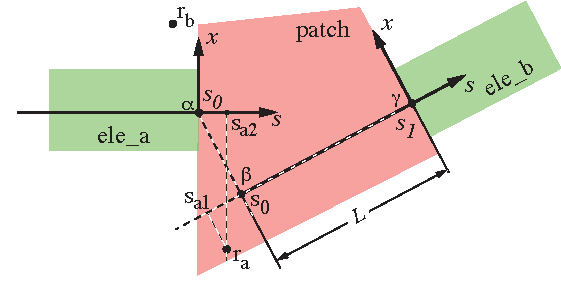
\includegraphics[width=5in]{patch-problem.pdf}
  \caption[The machine reference coordinates in a \vn{patch} element.]
{The machine reference coordinates in a \vn{Patch} element. The \vn{patch} element, shown
schematically as an irregular quadrilateral, is sandwiched between elements \vn{ele_a} and
\vn{ele_b}. \vn{L} is the length of the \vn{patch}. In this example, the \vn{patch} has a finite
\vn{y_rot}.}
  \label{f:patch.prob}
\end{figure}

%-----------------------------------------------------------------------------
%-----------------------------------------------------------------------------
\subsection{Patch Element Coordinates}
\label{s:patch.prob}
\index{patch}

Generally, if a particle is reasonably near the reference orbit, there is a one-to-one mapping
between the particle's position and $(x, y, s)$ coordinates. A \vn{patch} (\sref{s:patch}) elements
with a non-zero \vn{x_rot} or non-zero \vn{y_rot} breaks the one-to-one mapping. This is
illustrated in \fig{f:patch.prob}.  The \vn{patch} element, shown schematically as an, irregular
quadrilateral, is sandwiched between elements \vn{ele_a} and \vn{ele_b}. The machine coordinate system
with origin at $\alpha$ are the coordinates at the end of \vn{ele_a}. The coordinates at the end of
the \vn{patch} has its origin labeled $\gamma$. By convention, the length of the patch \vn{L} is
taken to be the longitudinal distance from $\alpha$ to $\gamma$ with the \vn{patch}'s exit
coordinates defining the longitudinal direction. The ``beginning'' point of the \vn{patch} on the
reference orbit a distance \vn{L} from point $\gamma$ is labeled $\beta$ in the figure.

In the machine $(x, y, s)$ coordinate system a particle at $\alpha$ will have some value $s = s_0$. A
particle at point $\beta$ will have the same value $s = s_0$ and a particle at $\gamma$ will have $s
= s_1 = s_0 + L$. A particle at point $r_a$ in \fig{f:patch.prob} illustrates the problem of
assigning $(x, y, s)$ coordinates to a given position. If the particle is considered to be within
the region of \vn{ele_a}, the particle's $s$ position will be $s_{a2}$ which is greater than the
value $s_0$ at the exit end of the element. This contradicts the expectation that particles within
\vn{ele_a} will have $s \le s_0$.  If, on the other hand, the particle is considered to be within
the \vn{patch} region, the particle's $s$ position will be $s_{a1}$ which is less than the value
$s_0$ at the entrance to the patch. This contradicts the expectation that a particles within the
\vn{patch} will have $s \ge s_0$.

To resolve this problem, \bmad considers a particle at position $r_a$ to be within the \vn{patch}
region. This means that there is, in theory, no lower limit to the $s$-position that a particle in
the \vn{patch} region can have. This also implies that there is a discontinuity in the $s$-position
of a particle crossing the exit face of \vn{ele1}. Typically, when particles are translated from the
exit face of one element to the exit face of the next, this \vn{patch} problem does not appear. It
only appears when the track between faces is considered.

Notice that a particle at position $r_b$ in \fig{f:patch.prob} can simultaneously be considered to
be in either \vn{ele_a} or the \vn{patch}. While this creates an ambiguity it does not complicate
tracking.

%-----------------------------------------------------------------------------
\section{Global Coordinates}
\label{s:global}
\index{global coordinates|hyperbf}

\begin{figure}[tb]
  \centering
  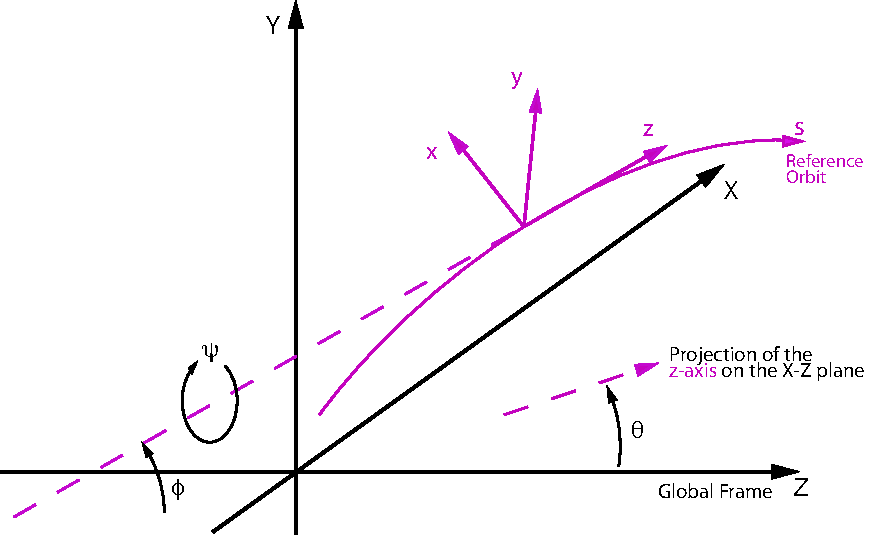
\includegraphics{global-coords.pdf}
  \caption[The Global Coordinate System]{
The machine (reference) coordinate system (purple), which is a function of $s$ along the reference
orbit, is described in the global coordinate system (black) by a position $(X(s), Y(s), Z(s))$ and
and by angles $\theta(s)$, $\phi(s)$, and $\psi(s)$.
  }
  \label{f:global.coords}
\end{figure}

The Cartesian \vn{global} coordinate system, also called the `floor'' coordinate system, is the
coordinate system ``attached to the earth'' that is used to describe the machine coordinate
system. Following the \mad\ convention, the \vn{global} coordinate axis are labeled $(X, Y,
Z)$. Conventionally, $Y$ is the ``vertical'' coordinate and $(X, Z)$ are the ``horizontal''
coordinates. To describe how the machine coordinate system is oriented within the global coordinate
system, each point on the $s$-axis of the machine coordinate system is characterized by its $(X, Y,
Z)$ position and by three angles $\theta(s)$, $\phi(s)$, and $\psi(s)$ that describe the orientation
of the machine coordinate axes as shown in \fig{f:global.coords}. These three angles are defined as
follows:
\begin{description}
%
\item[$\theta(s)$ Azimuth (yaw) angle:] 
Angle in the $(X, Z)$ plane between the $Z$--axis and the projection of the $z$--axis onto the $(X,
Z)$ plane. Corresponds to the \vn{y_rot} element parameter (\sref{s:offset}). A positive angle of
$\theta = \pi/2$ corresponds to the projected $z$--axis pointing in the negative $X$-direction.
%
\item[$\phi(s)$ Pitch (elevation) angle:] 
Angle between the $z$--axis and the $(X,Z)$ plane. Corresponds to the \vn{x_rot} element parameter
(\sref{s:offset}). A positive angle of $\phi = \pi/2$ corresponds to the $z$--axis pointing in the
positive $Y$ direction.
%
\item[$\psi(s)$ Roll angle:] 
Angle of the $x$--axis with respect to the line formed by the intersection of the $(X, Z)$ plane
with the $(x, y)$ plane. Corresponds to the \vn{tilt} element parameter (\sref{s:offset}). A
positive $\psi$ forms a right--handed screw with the $z$--axis.
\end{description}

\index{beginning statement}
\index{reference orbit!origin in global coordinates}
\index{global coordinates!reference orbit origin}
By default, at $s = 0$, the reference orbit's origin coincides with the $(X, Y, Z)$ origin and the
$x$, $y$, and $z$ axes correspond to the $X$, $Y$, and $Z$ axes respectively. If the lattice has no
vertical bends (the \vn{ref_tilt} parameter (\sref{s:bend}) of all bends are zero), the $y$--axis
will always be in the vertical $Y$ direction and the $x$--axis will lie in the horizontal $(X,Z)$
plane. In this case, $\theta$ decreases as one follows the reference orbit when going through a
horizontal bend with a positive bending angle. This corresponds to $x$ pointing radially
outward. Without any vertical bends, the $Y$ and $y$ axes will coincide, and $\phi$ and $\psi$ will
both be zero. The \vn{beginning} statement (\sref{s:beginning}) in a lattice file can be use to
override these defaults.

\index{MAD}
Following \mad, the global position of an element is characterized by a vector $\bfV$
\begin{equation}
  \bfV = 
  \begin{pmatrix}
    X \\ Y \\ Z 
  \end{pmatrix}
\end{equation}
The orientation of an element is described by a unitary rotation matrix $\bfW$. The column vectors
of $\bfW$ are the unit vectors spanning the machine coordinate axes in the order $(x, y, z)$. $\bfW$
can be expressed in terms of the orientation angles $\theta$, $\phi$, and $\psi$ via the formula
\begin{align}
  \bfW &= \bfR_{y}(\theta) \; \bfR_{x}(-\phi) \; \bfR_{z}(\psi) 
  \label{wwww} \\
  &= \begin{pmatrix}
    \cos\theta \cos\psi - \sin\theta \sin\phi \sin\psi & 
        -\cos\theta \sin\psi - \sin\theta \sin\phi \cos\psi & 
         \sin\theta \cos\phi \\
    \cos\phi \sin\psi & \cos\phi \cos\psi & \sin\phi \\
   -\cos\theta \sin\phi \sin\psi - \sin\theta \cos\psi & 
         \sin\theta \sin\psi - \cos\theta \sin\phi \cos\psi & 
         \cos\theta \cos\phi 
  \end{pmatrix}
  \nonumber
\end{align}
where
\begin{equation}
  \bfR_{y}(\theta) = 
  \begin{pmatrix}
    \cos\theta  & 0 & \sin\theta \\
    0           & 1 & 0          \\
    -\sin\theta & 0 & \cos\theta 
  \end{pmatrix}, \quad
  \bfR_{x}(\phi) = 
  \begin{pmatrix}
    1 & 0 & 0                \\
    0 & \cos\phi & -\sin\phi \\
    0 & \sin\phi &  \cos\phi 
  \end{pmatrix}, \quad
  \bfR_{z}(\psi) = 
  \begin{pmatrix}
    \cos\psi & -\sin\psi & 0 \\
    \sin\psi &  \cos\psi & 0 \\
    0        &  0        & 1                
  \end{pmatrix}
  \label{wtt0t}
\end{equation}
Notice that these are Tait-Bryan angles and not Euler angles.

An alternative representation of the $\bfW$ matrix (or any other rotation matrix) is to specify the
axis $\Bf u$ (normalized to 1) and angle of rotation $\beta$
\begin{equation}
  \bfW = \begin{pmatrix}
    \cos \beta + u_x^2 \left(1 - \cos \beta \right) & 
    u_x \, u_y \left(1 - \cos \beta \right) - u_z \sin \beta & 
    u_x \, u_z \left(1 - \cos \beta \right) + u_y \sin \beta \\ 
    u_y \, u_x \left(1 - \cos \beta \right) + u_z \sin \beta & 
    \cos \beta + u_y^2\left(1 - \cos \beta \right) & 
    u_y \, u_z \left(1 - \cos \beta \right) - u_x \sin \beta \\ 
    u_z \, u_x \left(1 - \cos \beta \right) - u_y \sin \beta & 
    u_z \, u_y \left(1 - \cos \beta \right) + u_x \sin \beta & 
    \cos \beta + u_z^2\left(1 - \cos \beta \right)
  \end{pmatrix}
  \label{wctux2}
\end{equation}

%-----------------------------------------------------------------------------
\subsection{Lattice Element Positioning}
\label{s:ele.pos}

\index{MAD}
\bmad, again following \mad, computes $\bfV$ and $\bfW$ by starting at the first element of the
lattice and iteratively using the equations
\begin{align}
  \bfV_i &= \bfW_{i-1} \; \bfL_i + \bfV_{i-1}, 
    \label{vwlv} \\
  \bfW_i &= \bfW_{i-1} \; \bfS_i
    \label{wws}
\end{align}
$\bfL_i$ is the displacement vector for the $i$\Th element and matrix $\bfS_i$ is the rotation of
the machine reference system of the exit end with respect to the entrance end. For clarity, the
subscript $i$ in the equations below will be dripped. For all elements whose reference orbit through
them is a straight line, the corresponding $\bfL$ and $\bfS$ are
\begin{equation}
  \bfL = 
  \begin{pmatrix}
      0 \\ 0 \\ L
  \end{pmatrix},
  \quad
  \bfS = 
  \begin{pmatrix}
      1 & 0 & 0 \\ 
      0 & 1 & 0 \\
      0 & 0 & 1
  \end{pmatrix},
  \label{l00l}
\end{equation}
Where $L$ is the length of the element. 

%-----------------------------------------------------------------------

\begin{figure}
\centering 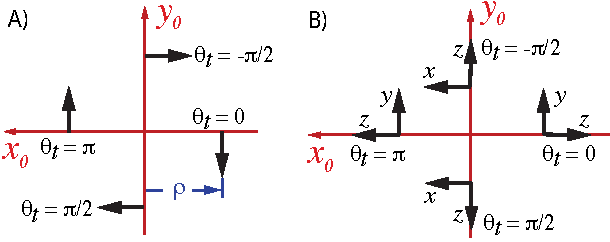
\includegraphics{tilt-bend.pdf} 
\caption[Orientation of a Bend.] 
  {
A) Rotation axes (bold arrows) for four different \vn{ref_tilt} angles of $\theta_t$ = 0, $\pm
\pi/2$, and $\pi$. $(x_0, y_0, z_0)$ are the machine coordinates at the entrance end of the bend with
the $z_0$ axis being directed into the page. Any rotation axis will be displaced by a distance of
the bend radius \vn{rho} from the origin. B) The $(x, y, z)$ coordinates at the exit end of the bend
for the same four \vn{ref_tilt} angles. In this case the bend angle is taken to be $\pi/2$.
  }
  \label{f:tilt.bend}
\end{figure}

%-----------------------------------------------------------------------

\index{rbend}\index{sbend}
\index{rho}\index{tilt}\index{angle}
For a \vn{bend}, the axis of rotation is dependent upon the bend's \vn{ref_tilt} angle
(\sref{s:offset}) as shown in \fig{f:tilt.bend}A. The axis of rotation points in the negative $y_0$
direction for \vn{ref_tilt} = 0 and is offset by the bend radius \vn{rho}. Here $(x_0, y_0, z_0)$
are the machine coordinates at the entrance end of the bend with the $z_0$ axis being directed into
the page in the figure.  For a non-zero \vn{ref_tilt}, the rotation axis is itself rotated about the
$z_0$ axis by the value of \vn{ref_tilt}. \fig{f:tilt.bend}B shows the exit coordinates for four
different values of \vn{ref_tilt} and for a bend angle \vn{angle} of $\pi/2$.  Notice that for a
bend in the horizontal $X-Z$ plane, a positive bend \vn{angle} will result in a decreasing azimuth
angle $\theta$.

For a bend, $\bfS$ is given using \Eq{wctux2} with 
\begin{align}
  \Bf u &= (-\sin\theta_t, -\cos\theta_t, 0) \CRNO
  \beta &= \alpha_b
  \label{ustt}
\end{align}
where $\theta_t$ is the \vn{ref_tilt} angle. The $\bfL$ vector for a \vn{bend} is given by 
\begin{equation}
  \bfL = \bfR_{z}(\theta_t) \; \bftilde L, \quad
  \bftilde L = 
  \begin{pmatrix}
    \rho (\cos\alpha_b - 1) \\ 0 \\ \rho \, \sin\alpha_b
  \end{pmatrix}
  \label{lrztt}
\end{equation}
where $\alpha_b$ is the bend \vn{angle} (\sref{s:bend}) and $\rho$ being the bend radius
(\vn{rho}). Notice that since $\Bf u$ is perpendicular to $z$, the curvilinear reference coordinate
system has no ``torsion''. That is, it is a Frenet-Serret coordinate system.

Note: An alternative equation for \vn{\bfS} for a bend is
 \begin{equation}
  \bfS = \bfR_{z}(\theta_t) \; \bfR_{y}(-\alpha_b) \; \bfR_{z}(-\theta_t)
  \label{srrr}
\end{equation}

The bend transformation above is so constructed that the transformation is equivalent to rotating
the machine coordinate system around an axis that is perpendicular to the plane of the bend. This
rotation axis is invariant under the bend transformation. For example, for $\theta_t = 0$ (or $\pi$)
the $y$-axis is the rotation axis and the $y$-axis of the machine coordinates before the bend will be
parallel to the $y$-axis of the machine coordinates after the bend as shown in \fig{f:tilt.bend}. That
is, a lattice with only bends with $\theta_t = 0$ or $\pi$ will lie in the horizontal plane (this
assuming that the $y$-axis starts out pointing along the $Y$-axis as it does by default).  For
$\theta_t = \pm\pi/2$, the bend axis is the $x$-axis. A value of $\theta_t = +\pi/2$ represents a
downward pointing bend.

\begin{figure}
  \centering 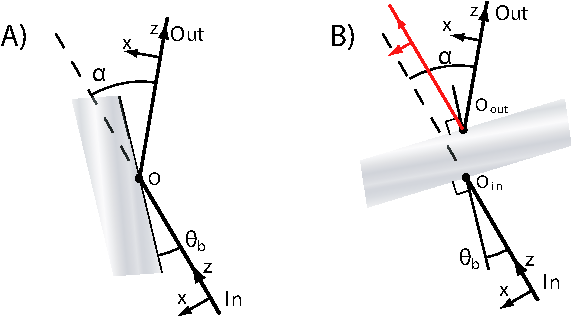
\includegraphics{mirror.pdf} 
\caption[Mirror and crystal geometry] {Mirror and crystal geometry.  The geometry shown here is
appropriate for a \vn{ref_tilt} angle of $\theta_t = 0$.  $\theta_g$ is the bend angle of the
incoming (entrance) ray, and $\alpha_b$ is the total bend angle of the reference trajectory. A)
Geometry for a mirror or a Bragg crystal. Point $\calO$ is the origin of both the machine coordinates
just before and just after the reflection/diffraction. B) Geometry for a Laue crystal.  Point
$\calO_{out}$ is the origin of the coordinates just after diffraction is displaced from the origin
$\calO_{in}$ just before diffraction due to the finite thickness of the crystal. here the bend
angles are measured with respect to the line that is in the plane of the entrance and exit
coordinates and perpendicular to the surface. For Laue diffraction, the user has the option of using
the undiffracted beam (shown in red) as the reference trajectory.
  }  
  \label{f:mirror}
\end{figure}

%-----------------------------------------------------------------------------
\subsection{Position Transformation When Transforming Coordinates}
\label{s:pos.trans}

A point $\bfQ_g = (X, Y, Z)$ defined in the global coordinate system, when expressed in the
coordinate system defined by $(\bfV, \bfW)$ is
\begin{equation}
  \bfQ_{VW} = \bfW^{-1} \left( \bfQ_g - \bfV \right)
  \label{rwrv}
\end{equation}
This is essentially the inverse of \Eq{vwlv}. That is, vectors propagate inversely to the
propagation of the coordinate system.

Using \Eq{rwrv} with \Eqs{vwlv}, and \eq{wws}, the transformation of a particle's position $\bfq =
(x,y,z)$ and momentum $\bfP = (P_x, P_y, P_z)$ when the coordinate frame is transformed from frame
$(\bfV_{i-1}, \bfW_{i-1})$ to frame $(\bfV_i, \bfW_i)$ is
\begin{align}
  \bfq_i &= \bfS_i^{-1} \, \left( \bfq_{i-1} - \bfL_i \right), 
    \label{rwlr} \\
  \bfP_i &= \bfS_i^{-1} \, \bfP_{i-1}
    \label{pps}
\end{align}

Notice that since $\bfS$ (and $\bfW$) is the product of orthogonal rotation matrices, $\bfS$ is
itself orthogonal and its inverse is just the transpose
\begin{equation}
  \bfS^{-1} = \bfS^T
\end{equation}

%-----------------------------------------------------------------------------
\subsection{Crystal and Mirror Element Coordinate Transformation}
\label{s:mirror.coords}

\index{crystal}\index{mirror}\index{ref_tilt}
A \vn{crystal} element (\sref{s:mirror}) diffracts photons and a \vn{mirror} element
(\sref{s:mirror}) reflects them. For a crystal setup for Bragg diffraction, and for a mirror, the
reference orbit is modeled as a zero length bend with $\bftilde L = (0, 0, 0)$, as shown in
\fig{f:mirror}A. Shown in the figure is the geometry appropriate for a \vn{ref_tilt} angle of
$\theta_t = 0$ (the rotation axis is here the $y$-axis). Since the mirror or crystal element is
modeled to be of zero length, the origin points (marked $\calO$ in the figure) of the entrance and
exit machine coordinates are the same. For Laue diffraction, the only difference is that $\bftilde L$
is non-zero due to the finite thickness of the crystal as shown in \fig{f:mirror}B. This results in
a separation between the entrance coordinate origin $\calO_{in}$ and the exit coordinate origin
$\calO_{out}$.

In all cases, the total bending angle is
\begin{align}
  \alpha_b &= \text{bragg_angle_in} + \text{bragg_angle_out} &&
                  \text{! Crystal, graze_angle_in} = 0 \CRNO
  \alpha_b &= \text{graze_angle_in} + \text{graze_angle_out} &&
                   \text{! Crystal, graze_angle_in} \ne 0 \CRNO
  \alpha_b &= 2 \, \text{graze_angle}                        &&\text{! Mirror}
  \label{agg}
\end{align}
With a mirror or Bragg diffraction, the bend angles are measured with respect to the surface
plane. With Laue diffraction the bend angles are measured with respect to the line in the bend plane
perpendicular to the surface.

For Laue diffraction, the user has the option of using the undiffracted beam (shown in red) as the
reference trajectory.

The orientation of the exit coordinates (the machine coordinates after the reflection) are only
affected by the element's \vn{ref_tilt} and bend angle parameters and is independent of all other
parameters such as the radius of curvature of the surface, etc. The machine $z$-axis of the entrance
coordinates along with the $z$-axis of the exit coordinates define a plane which is called the
element's \vn{bend plane}.  For a mirror, the graze angle is a parameter supplied by the user. For a
crystal, the Bragg angles are calculated so that the reference trajectory is in the middle of the
Darwin curve. Calculation of the Bragg angles for a crystal is given in
Section~\sref{s:crystal.ref}.

%-----------------------------------------------------------------------------
\subsection{Patch and FloorShift Elements Entrance to Exit Transformation}
\label{s:patch.coords}

\index{patch!coordinate transformation}\index{floorshift!coordinate transformation}
For \vn{patch} (\sref{s:patch}) and \vn{FloorShift} (\sref{s:floor.ele}) elements, the shift in the
exit end reference coordinates is given by \Eqs{vwlv} and \eq{wws} with
\begin{align}
  \bfL &= 
    \begin{pmatrix} 
      \text{x_offset} \\ \text{y_offset} \\ \text{z_offset} 
    \end{pmatrix}
    \CRNO
  \bfS &= \bfR_{y} (\text{y_rot}) \; \bfR_{x} (\text{y_rot}) \; \bfR_{z} (\text{tilt})
  \label{swww}
\end{align}

The difference here between \vn{patch} and \vn{SloorShift} elements is that, with a \vn{patch}
element, the shift is relative to the exit end of the previous element while, for a \vn{FloorShift}
element, the shift is relative to the reference point on the origin element specified by the
\vn{origin_ele} parameter of the \vn{FloorShift}.

%-----------------------------------------------------------------------------
\subsection{Fiducial and Girder Elements Origin Shift Transformation}
\label{s:girder.coords}

\index{girder}\index{fiducial}
For \vn{fiducial} and \vn{girder} elements, the alignment of the
reference coordinates with respect to ``\vn{origin}'' coordinates is
analogous to \Eqs{swww}. Explicitly:
\begin{align}
  \bfL &= 
    \begin{pmatrix} 
      \text{dx_origin} \\ \text{dy_origin} \\ \text{dz_origin}
    \end{pmatrix}
    \CRNO
  \bfS &= \bfR_{y} (\text{dtheta_origin}) \; \bfR_{-x} (\text{dphi_origin}) \; 
    \bfR_{z} (\text{dpsi_origin})
\end{align}

%-----------------------------------------------------------------------------
\subsection{Reflection Patch}
\label{s:reflect.patch}
\index{patch!reflection}

A \vn{Patch} (or a series of patches) that reflects the direction of the \vn{z}-axis is called a
\vn{reflection} \vn{patch}. By ``reflected direction'' it is meant that the dot product $\Bf z_1
\cdot \Bf z_2$ is negative where $\Bf z_1$ is the $z$-axis vector at the \vn{entrance} face and $\Bf
z_2$ is the $z$-axis vector at the \vn{exit} face. This condition is equivalent to the condition
that the associated $\bfS$ matrix (see \Eq{swww}) satisfy:
\begin{equation}
  S(3,3) < 0
  \label{s330}
\end{equation}
Using \Eq{swww} gives, after some simple algebra, this condition is equivalent to
\begin{equation}
  \cos(\text{x_rot}) \, \cos(\text{y_rot}) < 0
\end{equation}
When there are a series of patches, The transformations of all the patches are concatenated together
to form an effective $\bfS$ which can then be used with \Eq{s330}.

%-----------------------------------------------------------------------------
\section{Transformation Between Machine and Element Body Coordinates}
\label{s:lab.body.transform}
\index{machine coordinates}
\index{element body coordinates|hyperbf}

The \vn{element body} coordinates are the coordinate system attached to an element. Without any
misalignments, where \vn{``misalignments''} are here defined to be any offset, or rotation
(\sref{s:offset}), the \vn{machine} coordinates (\sref{s:ref}) and \vn{element body} coordinates
are the same. With misalignments, the transformation between \vn{machine} and \vn{element body}
coordinates depends upon whether the machine coordinate system is straight (\sref{s:straight.mis}) or
bent (\sref{s:bend.mis}).

When tracking a particle through an element, the particle starts at the \vn{nominal}
(\sref{s:coords}) upstream end of the element with the particle's position expressed in machine
coordinates. Tracking from the the nominal upstream end to the actual upstream face of the element
involves first transforming to element body coordinates (with $s = 0$ in the equations below) and
then propagating the particle as in a field free drift space from the particle's starting position
to the actual element face. Depending upon the element's orientation, this tracking may involve
tracking backwards. Similarly, after a particle has been tracked through the physical element to the
actual downstream face, the tracking to the nominal downstream end involves transforming to
machine coordinates (using $s = L$ in the equations below) and then propagating the particle as
in a field free drift space to the nominal downstream edge.

%-----------------------------------------------------------------------------
\subsection{Straight Element Misalignment Transformation}
\label{s:straight.mis}

For straight line elements, given a machine coordinate frame $\Lambda_s$ with origin a distance
$s$ from the beginning of the element, misalignments will shift the coordinates to a new reference
frame denoted $E_s$. Since misalignments are defined with respect to the middle of the element, the
transformation between $\Lambda_s$ and $E_s$ is a three step process:
\begin{equation}
  \Lambda_s \longrightarrow \Lambda_\text{mid} 
  \longrightarrow E_\text{mid} \longrightarrow E_s
  \label{llee}
\end{equation}
where $\Lambda_\text{mid}$ and $E_\text{mid}$ are the machine and element reference frames at the
center of the element.

The first and last transformations from $\Lambda_s$ to $\Lambda_\text{mid}$ and from $E_\text{mid}$
to $E_s$ use \Eqs{vwlv}, \eq{wws}, and \eq{l00l} with the replacement $L \rightarrow L/2 - s$ for
the first transformation and $L \rightarrow s - L/2$ for the third transformation. The middle
transformation, by definition of the offset and rotation parameters is
\begin{align}
  \bfL &= 
    \begin{pmatrix} 
      \text{x_offset} \\ \text{y_offset} \\ \text{z_offset} 
    \end{pmatrix}
    \CRNO
  \bfS &= \bfR_{y} (\text{x_rot}) \; \bfR_{x} (\text{y_rot}) \; \bfR_{z} (\text{tilt})
  \label{swww2}
\end{align}

Notice that with this definition of how elements are misaligned, the position of the center of a
non-bend misaligned element depends only on the offsets, and is independent of the rotations.

%-----------------------------------------------------------------------------
\subsection{Bend Element Misalignment Transformation}
\label{s:bend.mis}

This needs cleanup!!!

\index{rbend!coordinate transformation}\index{sbend!coordinate transformation}
\index{roll!coordinate transformation}\index{tilt!coordinate transformation}
For \vn{rbend} and \vn{sbend} elements there is no \vn{tilt} parameter.  Rather, there is the
\vn{roll} parameter and a \vn{ref_tilt} parameter. The latter affects both the reference orbit and
the bend position (\sref{s:bend.orient}). Furthermore, \vn{ref_tilt} is calculated with respect to
the coordinates at the beginning of the bend while, like straight elements, \vn{roll}, \vn{x_rot},
\vn{y_rot}, and offsets are calculated with respect to the center of the bend. 
The different reference frame used
for \vn{ref_tilt} versus everything else means that five transformations are needed to get from the
machine frame to the element body frame (see \Eq{llee}). Symbolically:
\begin{equation}
  \Lambda_s \longrightarrow \Lambda_\text{mid} 
  \longrightarrow \Omega_\text{mid} \longrightarrow \Omega_0
  \longrightarrow E_0 \longrightarrow E_s
\end{equation}

The first transformation, $\Lambda_s$ to $\Lambda_\text{mid}$, from machine coordinates at a
distance $s$ from the beginning of the element to machine coordinates at the center the bend is a
rotation around the center of curvature of the bend and is given by \Eqs{vwlv} and \eq{wws} with
\Eqs{ustt} and \eq{lrztt} with the substitution $\alpha_b \rightarrow (L/2 - s)/\rho$.

The second transformation $\Lambda_\text{mid}$ to $\Omega_\text{mid}$ at the center of the element
adds in the misalignments (Note that the coordinate frame $\Omega_\text{mid}$ is neither a
machine frame or an element frame so hence the use of a different symbol $\Omega$). Explicitly,
the $\Lambda_\text{mid} \longrightarrow \Omega_\text{mid}$ transformation is
\begin{align}
  \bfL &= \bfL_\text{off} + 
    \left[ \bfR_z(\text{roll}) - \Bf1 \right] \; \bfR_z(\theta_t) \; \bfR_{y}(\alpha_b/2) \; 
      \bfL_c \CRNO
  \bfS &= \bfR_{y}(\text{y_rot}) \; \bfR_{x}(\text{x_rot}) \; \bfR_z(\text{roll})
  \label{lcmis}
\end{align}
where
\begin{equation}
  \bfL_c = 
    \begin{pmatrix}
      \rho (\cos(\alpha_b/2) - 1) \\ 0 \\ \rho \, \sin(\alpha_b/2)
    \end{pmatrix}
  , \qquad
  \bfL_\text{off} = 
    \begin{pmatrix} 
      \text{x_offset} \\ \text{y_offset} \\ \text{z_offset} 
    \end{pmatrix}
\end{equation}
The reason why $\bfL$ has a different form from straight line elements is due to the fact that the
axis of rotation for a \vn{roll} is displaced from the $z$-axis of the coordinate system at the
center of the bend (see \fig{f:roll}).

The third transformation from $\Omega_\text{mid}$ to $\Omega_0$ is like the first transformation and
rotates from the center of the bend to the beginning. Again \Eqs{ustt} and \eq{lrztt} are used with
the substitution $\alpha_b \rightarrow -L/2\rho$.

The fourth transformation $\Omega_0$ to $E_0$ tilts the reference frame by an amount \vn{ref_tilt}:
\begin{equation}
  \bfL = 0, \quad
  \bfS = \bfR_{z}(\theta_t)
  \label{l0sr}
\end{equation}

The fifth and final transformation, $E_0$ to $E_s$, like the first and third, rotates around the
center of the bend but in this case, since we are dealing with element coordinates, the
\vn{ref_tilt} is ignored.  That is, \Eqs{ustt} and \eq{lrztt} are used with the substitutions
$\theta_t \rightarrow 0$ and $\alpha_b \rightarrow L/\rho$.

Notice that with this definition of how elements are misaligned, the position of the center of a
misaligned element depends only on the offsets and \vn{roll}, and is independent of any rotations. 
Also the orientation of an element depends only on the \vn{x_rot}, \vn{y_rot}, \vn{roll}, 
and \vn{ref_tilt}, and is independent of the offsets.

%-----------------------------------------------------------------------------
\section{Phase Space Coordinates}
\label{s:phase.coords}
\index{phase space coordinates|hyperbf}

%-----------------------------------------------------------------------------
\subsection{Reference Particle, Reference Energy, and Reference Time}
\label{s:ref.energy}
\index{reference particle|hyperbf}
\index{reference energy|hyperbf}
\index{reference time|hyperbf}

The \vn{reference energy} and \vn{reference time} are needed in evaluating the phase space
coordinates of charged particles (\sref{s:phase.space}).

All lattice elements, except for controller elements, have an associated \vn{reference energy}
energy.  The reference energy at the start of a lattice's \vn{root branch} (\sref{s:branch.def}) is
set in the lattice file by setting the reference momentum (\vn{p0c}) or total energy (\vn{E_tot})
using a \vn{parameter} (\sref{s:param}) or \vn{beginning} (\sref{s:beginning}) statement. For other
branches, the energy at the start of the branch is set using the appropriate line parameter
(\sref{s:beginning}) statement.

Note that the reference momentum \vn{p0c} is actually the reference momentum times the speed of light
so that the reference momentum has the same unit (eV) as the reference energy.

\index{custom!reference energy}\index{em_field!reference energy}
\index{hybrid!reference energy}\index{lcavity!reference energy}
\index{patch!reference energy}
For most elements, the reference energy is the same as the reference energy of the proceeding
element. The following elements are exceptions:
\begin{example}
  custom
  em_field
  hybrid
  lcavity
  patch
\end{example}
The reference energy of these elements is determined by tracking a particle (the ``\vn{reference
particle}'') through the element with the particle starting on the reference orbit and whose energy
is equal to the reference energy. The energy of the particle at the downstream end is the reference
energy of the element. Note: Tracking through an element to determine the reference energy is always
done with the element turned on independent of the setting of the element's \vn{is_on}
(\sref{s:is.on}) parameter. Reference energy tracking is also done ignoring any orientation parameters
(\sref{s:offset}) and errors like \vn{voltage_err}.

\index{wiggler!reference time}
Besides the reference energy, lattice elements have an associated \vn{reference time} which is
computed, for most elements, by the time-of-flight of the \vn{reference particle} assuming that the
reference particle is following the reference orbit. Exceptions are \vn{wiggler} elements which uses
the time-of-flight of the actual undulating trajectory. [Actually what is used in the computation of
the $z$ phase space coordinate (\Eq{zbctt}) is the sum of reference time deltas of the elements that
a particle has passed through. It is not possible to assign a unique reference time to an element
when particles are recirculating through elements as in a storage ring.]

%-----------------------------------------------------------------------------
\subsection{Charged Particle Phase Space Coordinates}
\label{s:phase.space}
\index{phase space coordinates|hyperbf}

\begin{figure}
\centering 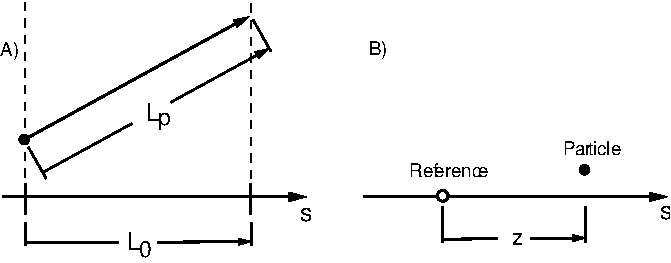
\includegraphics{canonical-z.pdf} \caption[Interpreting phase space $z$ at constant
velocity.]  {Interpreting phase space $z$ at constant velocity: A) The change in $z$ going through
an element of length $L_0$ is $L_0 - L_p$.  B) At constant time, $z$ is the longitudinal distance
between the reference particle and the particle.}  \label{f:canonical.z}
\end{figure}

For charged particles (more correctly, for everything but photons (\sref{s:photon.phase.space})),
\bmad uses the canonical phase space coordinates
\begin{equation}
  \Bf r(s) = (x, p_x, y, p_y, z, p_z)
\end{equation}
The longitudinal position $s$ is the independent variable instead of the time. $x$ and $y$, are the
transverse coordinates of the particle as shown in~\fig{f:machine.coords}A. Note that $x$ and $y$ are
independent of the position of the reference particle.

The phase space momenta $p_x$ and $p_y$ are normalized by the reference (sometimes called the
design) momentum $P_0$
\begin{equation}
  p_x = \frac{P_x}{P_0}, \qquad
  p_y = \frac{P_y}{P_0}
  \label{ppp}
\end{equation}
where $P_x$ and $P_y$ are respectively the $x$ and $y$ momentums.

\index{lcavity}\index{rfcavity}
The phase space $z$ coordinate is 
\begin{align}
  z(s) &= -\beta(s) \, c \, (t(s) - t_0(s)) \CRNO
    &\equiv - \beta(s) \, c \, \Delta t(s)
  \label{zbctt}
\end{align}
$t(s)$ is the time at which the particle is at position $s$, $t_0(s)$ is the time at which the
reference particle is at position $s$, and $\beta$ is $v/c$ with $v$ being the particle velocity
(and not the reference velocity). The reference particle is, by definition, ``synchronized'' with
elements whose fields are oscillating and therefore the actual fields a particle will see when
traveling through such an element will depend upon the particle's phase space $z$. For example, the
energy change of a particle traveling through an \vn{lcavity} (\sref{s:lcav}) or \vn{rfcavity}
(\sref{s:rfcav}) element is $z$ dependent. Exception: With absolute time tracking (\sref{s:rf.time})
fields are tied to the absolute time and not $z$.

If the particle's velocity is constant, and is the same as the velocity of the reference particle
(for example, at high energy where $\beta = 1$ for all particles), then $\beta \, c \, t$ is just
the path length. In this case, the change in $z$ going through an element is
\begin{equation}
  \Delta z = L_0 - L_p
\end{equation}
where, as shown in \fig{f:canonical.z}A, $L_0$ is the path length of the reference particle (which
is just the length of the element) and $L_p$ is the path length of the particle in traversing the
element.  Another way of interpreting phase space $z$ is that, at constant $\beta$, and constant
time, $z$ is the longitudinal distance between the particle and the reference particle as shown in
\fig{f:canonical.z}B. with positive $z$ indicating that the particle is ahead of the reference
particle.

Do not confuse the phase space $z$ with the $z$ that is the particle's longitudinal coordinate in
the machine reference frame as shown in \fig{f:machine.coords}. By construction, this latter $z$ is
always zero.

Notice that if a particle gets an instantaneous longitudinal kick so that $\beta$ is discontinuous
then, from \Eq{zbctt}, phase space $z$ is discontinuous even though the particle itself does not
move in space. In general, from \Eq{zbctt}, The value of $z$ for a particle at $s_2$ is related to
the value of $z$ for the particle at $s_1$ by
\begin{equation}
  z_2 = \frac{\beta_2}{\beta_1} \, z_1 - 
  \beta_2 \, c \, (\Delta t_2 - \Delta t_1)
  \label{zbbzb}
\end{equation}
$\Delta t_2 - \Delta t_1$ can be interpreted as the difference in transit time, between the particle
and the reference particle, in going from $s_1$ to $s_2$.

The longitudinal phase space momentum $p_z$ is given by
\begin{equation}
  p_z = \frac{\Delta P}{P_0} \equiv \frac{P - P_0}{P_0}
  \label{ppppp}
\end{equation}
where $P$ is the momentum of the particle. For ultra--relativistic particles $p_z$ can be
approximated by
\begin{equation}
  p_z = \frac{\Delta E}{E_0}
\end{equation}
\index{lcavity}
where $E_0$ is the reference energy (energy here always refers to the total energy) and $\Delta E =
E - E_0$ is the deviation of the particle's energy from the reference energy. For an \vn{Lcavity}
element (\sref{s:lcav}) the reference momentum is {\it not} constant so the tracking for an
\vn{Lcavity} is not canonical.

\index{phase space coordinates!MAD convention}
\index{MAD!phase space convention}
\mad uses a different coordinate system where $(z, p_z)$ is replaced by $(-c\Delta t, p_t)$ where
$p_t \equiv \Delta E / P_0 c$. For highly relativistic particles the two coordinate systems are
identical.

\index{paraxial approximation}
\index{bmad_standard!tracking method}
The relationship, between the phase space momenta and the slopes $x' \equiv dx/ds$ and 
$y' \equiv dy/ds$ is
\begin{align}
  x' &= \frac{p_x}{\sqrt{(1 + p_z)^2 - p_x^2 - p_y^2}} \, (1 + g x) \\
  y' &= \frac{p_y}{\sqrt{(1 + p_z)^2 - p_x^2 - p_y^2}} \, (1 + g x) 
  \label{xpa1p}
\end{align}
$g = 1/\rho$ is the curvature function with $\rho$ being the radius of curvature of the reference
orbit and it has been assumed that the bending is in the $x$--$z$ plane.

With the paraxial approximation, and in the relativistic limit, the change in $z$ with position is
\begin{equation}
  \frac{dz}{ds} = -g \, x - \frac{1}{2} (x'^2 + y'^2)
\end{equation}
This shows that in a linac, without any bends, the $z$ of a particle always decreases.

A particle can also have a spin. The spin is characterized by the spinor $\Psi = \left( \psi_{1},
\psi_{2} \right)^{T}$ where $\psi_{1,2}$ are complex numbers (\sref{s:spin.dyn}).

%-----------------------------------------------------------------------------
\subsection{Time-based Phase Space Coordinates}
\label{s:time.phase.space}
\index{time!phase space coordinates|hyperbf}

Some specialized routines (for example, time Runge Kutta tracking) use the time $t$ as the
independent variable for charged particle tracking. This is useful when particles can reverse
direction since the normal $z$ based tracking cannot handle this. Direction reversal can happen, for
example, with low energy ``dark current'' electrons that are generated at the walls of the vacuum
chamber.

When the tracking is time based the phase space coordinates are:
\begin{equation}
  (x, c \, p_x, y, c \, p_y, z, c \, p_s)
\end{equation}
The positions $x$, $y$, and $z$ are the same as with phase space coordinates
(\sref{s:phase.space}). The momenta are defined as
\begin{align}
c p_x &\equiv m c^2 \gamma \beta_x \CRNO
c p_y &\equiv m c^2 \gamma \beta_y \\
c p_s &\equiv m c^2 \gamma \beta_s, \nonumber
\end{align}
and internally are stored in units of eV.

%-----------------------------------------------------------------------------
\subsection{Photon Phase Space Coordinates}
\label{s:photon.phase.space}
\index{photon!phase space coordinates|hyperbf}

The phase space coordinates discussed above implicitly assume that
particles are traveling longitudinally in only one direction. That is,
the sign of the $s$ component of the momentum cannot be determined
from the phase space coordinates. This is generally fine for tracking
high energy beams of charged particles but for photon tracking this
would oftentimes be problematical. For photons, therefore, a different
phase space is used:
\begin{equation}
  (x, \beta_x, y, \beta_y, z, \beta_z)
  \label{xbybzb}
\end{equation}
Here $(\beta_x, \beta_y, \beta_z)$ is the normalized photon velocity with
\begin{equation}
  \beta_x^2 + \beta_y^2 + \beta_z^2 = 1 
  \label{bbb1}
\end{equation}
and $(x, y, z)$ are the reference orbit coordinates with $z$ being the
distance from the start of the lattice element the photon is in.

In \bmad, the information associated with a photon include its phase
space coordinates and time along with the photon energy and four
parameters $E_x, \phi_x$, and $E_y, \phi_y$ specifying the intensity
and phase of the field along the $x$ and $y$ axes transverse to the
direction of propagation.  the field in the vicinity of the photon is
\begin{align}
  E_x (\Bf r, t) &\sim E_x \, e^{i (k \, (z - z_0) - \omega \, (t - t_\REF) + \phi_x)} \CRNO
  E_y (\Bf r, t) &\sim E_y \, e^{i (k \, (z - z_0) - \omega \, (t - t_\REF) + \phi_y)} 
  \label{ertee}
\end{align}
where $z_0$ is the photon $z$ position and and $t_\REF$ is the reference time.

The normalization between field and intensity is dependent upon the
particular parameters of any given simulation and so must be
determined by the program using \bmad.


\chapter{Electromagnetic Fields}

%-----------------------------------------------------------------
\section{Magnetostatic Multipole Fields}
\label{s:mag.field}
\index{magnetic fields|hyperbf}

\index{MAD}
Start with the assumption that the local magnetic field has no longitudinal component
(obviously this assumption does not work with, say, a solenoid).  Following \mad, ignoring
skew fields for the moment, the vertical magnetic field along the $y = 0$ axis is expanded
in a Taylor series
\begin{equation}
  B_y(x, 0) = \sum_n B_n \, \frac{x^n}{n!}
  \label{byx0b}
\end{equation}
Assuming that the reference orbit is locally straight (there are correction terms if the
reference orbit is curved (\sref{s:field.exact})), the field is
\begin{alignat}{5}
  B_x &=           &&B_1 y \plus         &&B_2 \, xy       
                   && \plus && \frac{1}{6} B_3 (3x^2 y - y^3) \plus \ldots \CRNO
  B_y &= B_0 \plus &&B_1 x + \frac{1}{2} &&B_2 (x^2 - y^2) 
                   && \plus && \frac{1}{6} B_3 (x^3 - 3x y^2) \plus \ldots
  \label{bbb}
\end{alignat}
The relation between the field $B_n$ and the normalized field $K_n$ is:
\index{multipole!KnL, Tn|hyperbf}
\begin{equation}
  K_n \equiv \frac{q \, B_n}{P_0}
  \label{kqlbp}
\end{equation}
where $q$ is the charge of the reference particle (in units of the elementary charge), and $P_0$ is
the reference momentum (in units of eV/c).  Note that $P_0/q$ is sometimes written as $B\rho$. This
is just an old notation where $\rho$ is the bending radius of a particle with the reference energy
in a field of strength $B$. Notice that $P_0$ is the local reference momentum at the element which
may not be the same as the reference energy at the beginning of the lattice if there are
\vn{lcavity} elements (\sref{s:lcav}) present.

The kicks $\Delta p_x$ and $\Delta p_y$ that a particle experiences going through a multipole field
is
\begin{alignat}{5}
  \Delta p_x & = \frac{-q \, L \, B_y}{P_0} \label{pqlbp1} \\
             & = -K_0 L \;-\; 
             && K_1 L \, x \plus 
             \frac{1}{2} && K_2 L (y^2 - x^2) && \plus 
             && \frac{1}{6} K_3 L (3x y^2 - x^3) \plus \ldots 
             \nonumber \\
  \Delta p_y & = \frac{q \, L \, B_x}{P_0} \label{pqlbp2} \\
             & =     
             && K_1 L \, y \plus 
             && K_2 L \, xy && \plus 
             && \frac{1}{6} K_3L (3x^2 y - y^3) \plus \ldots \nonumber 
\end{alignat}
A positive $K_1L$ quadrupole component gives horizontal focusing and vertical defocusing. The
general form is
\begin{align}
  \Delta p_x &= \sum_{n = 0}^{\infty} \frac{K_n L}{n!} 
             \sum_{m = 0}^{2m \le n}
             \begin{pmatrix} n \cr 2m \end{pmatrix} \,
             (-1)^{m+1} \, x^{n-2m} \, y^{2m} \\
  \Delta p_y &= \sum_{n = 0}^{\infty} \frac{K_n L}{n!} 
             \sum_{m = 0}^{2m \le n-1}
             \begin{pmatrix} n \cr 2m+1 \end{pmatrix} \,
             (-1)^{m} \, x^{n-2m-1} \, y^{2m+1}
\end{align}
where $\binom{a}{b}$ (``a choose b'') denotes a binomial coefficient.

\index{multipole!KnL, Tn|hyperbf}
The above equations are for fields with a normal component only. If a given multipole field of order
$n$ has normal $B_n$ and skew $S_n$ components and is rotated in the $(x, y)$ plane by an angle
$T_n$, the magnetic field at a point $(x,y)$ can be expressed in complex notation as
\begin{equation}
  B_y(x,y) + i B_x(x,y) = 
    \frac{1}{n!} (B_n + i S_n) \, e^{-i(n+1)T_n} \, e^{i n \theta} \, r^n 
  \label{bib1nb}
\end{equation}
where $(r, \theta)$ are the polar coordinates of the point $(x, y)$.

\index{multipole}
Note that, for compatibility with MAD, the $K0L$ component of a \vn{Multipole} element rotates the
reference orbit essentially acting as a zero length bend. This is not true for multipoles of any
other type of element.

Instead of using magnitude $K_n$ and rotation angle $\theta_n$, Another representation is using
normal $\wt K_n$ and skew $\wt S_n$. The conversion between the two are
\begin{align}
  \wt K_n &= K_n \, \cos((n + 1) \, T_n) \CRNO
  \wt S_n &= K_n \, \sin((n + 1) \, T_n) 
\end{align}

\index{multipole!an, bn|hyperbf}
Another representation of the magnetic field used by \bmad divides the fields into normal $b_n$ and
skew $a_n$ components. In terms of these components the magnetic field for the $n$\Th\ order
multipole is
\begin{equation}
  \frac{q \, L}{P_0} \, (B_y + i B_x) = (b_n + i a_n) \, (x + i y)^n
  \label{qlpbb}
\end{equation}
The $a_n$, $b_n$ representation of multipole fields can be used in elements such as
quadrupoles, sextupoles, etc. to allow ``error'' fields to be represented.  
The conversion between $(a_n, b_n)$ and $(K_nL, S_nL, T_n)$ is
\begin{equation}
  b_n + i a_n = \frac{1}{n!} \, (K_nL + i \, S_nL) \, e^{-i(n+1)T_n}
\end{equation}
In the case where $S_nL = 0$
\begin{align}
  K_n L &= n! \, \sqrt{a_n^2 + b_n^2} \\
  \tan[(n+1) T_n] &= \frac{-a_n}{b_n}
\end{align}
To convert a normal magnet (a magnet with no skew component) into a skew magnet (a magnet with no
normal component) the magnet should be rotated about its longitudinal axis with a rotation angle of
\begin{equation}
  (n+1) T_n = \frac{\pi}{2}
\end{equation}
For example, a normal quadrupole rotated by $45^\circ$ becomes a skew quadrupole.

The multipole fields can be ``\vn{reference energy}'' scaled and/or ``\vn{element strength}''
scaled.  Scaling here means that the $a_n$ and $b_n$ values used in tracking are scaled from the
input values given in the lattice file.

\vn{Reference energy} scaling is applied if the \vn{field_master} attribute (\sref{s:field.master})
is True for an element so that the multipole values specified in the lattice file are not reference
energy normalized
\begin{equation}
  \bigl[ a_n, b_n \bigr] \longrightarrow
  \bigl[ a_n, b_n \bigr] \cdot \frac{q}{P_0}
  \label{ababq}
\end{equation}

\index{r0_mag}
\index{F (multipole scale factor)}
\vn{Element strength} scaling is applied when the multipoles are associated with a non
\vn{AB_Multipole} element and if the \vn{scale_multipoles} attribute (\sref{s:multip}) is
\vn{True}. This scaling uses a measurement radius $r_0$ and a scale factor $F$:
\begin{equation}
  \bigl[ a_n, b_n \bigr] \longrightarrow
  \bigl[ a_n, b_n \bigr]
  \cdot F \cdot \frac{r_0^{n_\REF}}{r_0^n}
  \label{ababf}
\end{equation}
$r_0$ is set by the \vn{r0_mag} attribute of an element. $F$ and $n_\REF$ are set
automatically depending upon the type of element as shown in Table~\ref{t:ab}. The
$\gamma_p$ term is

\index{kicker}\index{hkicker}\index{vkicker}\index{ac_kicker}
\index{rbend}\index{sbend}\index{elseparator}
\index{quadrupole}\index{solenoid}\index{sol_quad}
\index{sextupole}\index{octupole}
\begin{table}[ht]
\centering
\begin{tabular}{lll} \toprule
\tt
  {\em Element} & $F$                              & $n_\REF$ \\ \midrule
  \vn{Elseparator} & $\sqrt{{\tt Hkick}^2 + {\tt Vkick}^2}$ & 0 \\
  \vn{Hkicker}     & Kick                                   & 0 \\
  \vn{Kicker},\vn{AC_Kicker}
                   & $\sqrt{{\tt Hkick}^2 + {\tt Vkick}^2}$ & 0 \\
  \vn{Rbend}       & G * L                                  & 0 \\
  \vn{Sbend}       & G * L                                  & 0 \\
  \vn{Vkicker}     & Kick                                   & 0 \\
  \vn{Wiggler}     & $\dsfrac{2 \, c \, {\tt L\_pole} \, B_{max}}{\pi \, {\tt p0c}}$ 
                                                            & 0 \\
  \vn{Quadrupole}  & K1 * L                                 & 1 \\
  \vn{Sol_Quad}    & K1 * L                                 & 1 \\
  \vn{Solenoid}    & KS * L                                 & 1 \\
  \vn{Sextupole}   & K2 * L                                 & 2 \\
  \vn{Octupole}    & K3 * L                                 & 3 \\ \bottomrule
\end{tabular}
\caption{$F$ and $n_\REF$ for various elements.}
\label{t:ab}
\end{table}

%-----------------------------------------------------------------
\section{Electrostatic Multipole Fields}
\label{s:elec.field}
\index{electric fields}

Except for the \vn{elseparator} element, \bmad specifies DC electric fields using normal
$b_{en}$ and skew $a_{en}$ components (\sref{s:multip}). The potential $\phi_n$ for the
$n$\Th\ order multipole is
\begin{equation}
  \phi_n = -\re \left[ \frac{b_{en} - i a_{en}}{n + 1} \, \frac{(x + i y)^{n+1}}{r_0^n} \right]
  \label{pbian1}
\end{equation}
where $r_0$ is a ``measurement radius'' set by the \vn{r0_elec} attribute of an element
(\sref{s:multip}).

The electric field for the $n$\Th order multipole is
\begin{equation}
  E_x - i E_y = (b_{en} - i a_{en}) \, \frac{(x + i y)^n}{r_0^n}
  \label{exiey}
\end{equation}
Notice that the magnetic multipole components $a_n$ and $b_n$ are normalized by the
element length, reference charge, and reference momentum (\Eq{qlpbb}) while their electric
counterparts are not.

Using the paraxial approximation, The kick given a particle due to the electric field is
\begin{equation}
  \frac{dp_x}{ds} = \frac{q \, E_x}{\beta \, P_0 \, c}, \qquad \frac{dp_y}{ds} = \frac{q \, E_y}{\beta \, P_0 \, c}
\end{equation}
Where $\beta$ is the normalized velocity.

%-----------------------------------------------------------------
\section{Exact Multipole Fields in a Bend}
\label{s:field.exact}

For static magnetic and electric multipole fields in a bend, the spacial dependence of the
field is different from multipole fields in an element with a straight geometry as given
by \Eqs{qlpbb} and \eq{exiey}. The analysis of the multipole fields in a bend here follows
McMillan\cite{McMillan:Multipoles}.  

In the rest of this section, normalized coordinates $\rw = r / \rho$, $\xw / = x /
\rho$, and $\yw = y / \rho$ will be used where $\rho$ is the bending radius of the
reference coordinate system, $r$ is the distance, in the plane of the bend, from the bend
center to the observation point, $x$ is the distance in the plane of the from the reference
coordinates to the observation point and $y$ is the distance out-of-plane. With this
convention $\rw = 1 + \xw$.

An electric or magnetic multipole can be characterized by a scalar potential $\phi$ with
the field given by $-\nabla \phi$.  The potential is a solution to Laplace's equation
\begin{equation}
  \frac{1}{\rw} \, \frac{\partial}{\partial \, \rw} 
  \left( \rw \, \frac{\partial \, \phi}{\partial \, \rw} \right) +
  \frac{\partial^2 \phi}{\partial \, \yw^2} = 0
\end{equation}
As McMillian shows, it is also possible to calculate the magnetic field by constructing the
appropriate vector potential. However, from a practical point of view, it is simpler to use the
scalar potential for both the magnetic and electric fields.

Solutions to Laplace's equation can be found in form
\begin{equation}
  \phi_{n}^r = \frac{-1}{1+n} \sum_{p = 0}^{2p \le n+1} 
             \begin{pmatrix} n + 1 \cr 2 \, p \end{pmatrix} \,
             (-1)^{p} \, F_{n+1-2p}(\rw) \, \yw^{2p}
  \label{pspn1}
\end{equation}
and in the form
\begin{equation}
  \phi_{n}^i = \frac{-1}{1+n} \sum_{p = 0}^{2p \le n}
             \begin{pmatrix} n + 1 \cr 2p +1 \end{pmatrix} \,
             (-1)^{p} \, F_{n-2p}(\rw) \, \yw^{2p+1}
  \label{pspn2}
\end{equation}
where $\binom{a}{b}$ (``a choose b'') denotes a binomial coefficient, and $n$ is the order
number which can range from 0 to infinity.\footnote
  { 
Notice that here $n$ is related to $m$ in
McMillian's paper by $m = n + 1$. Also note that the $\phi^r$ and $\phi^i$ here have a
normalization factor that is different from McMillian.
  }

In \Eq{pspn2} the $F_p(\rw)$ are related by
\begin{equation}
  F_{p+2} = (p + 1) \, (p + 2) \, \int_1^{\rw} \frac{d\rw}{\rw} 
  \left[ \int_1^{\rw} d\rw \, \rw \, F_{p} \right]
\end{equation}
with the ``boundary condition'':
\begin{align}
  F_0(\rw) &= 1 \CRNO
  F_1(\rw) &= \ln \, \rw
\end{align}
This condition ensures that the number of terms in the sums in \Eqs{pspn1} and \eq{pspn2}
are finite. With this condition, all the $F_p$ can be constructed:
\begin{align}
  F_1 &= \ln \, \rw = \xw - \frac{1}{2}\xw^2 + \frac{1}{3}\xw^3 - \ldots \CRNO
  F_2 &= \frac{1}{2} (\rw^2 - 1) - \ln \rw = \xw^2 - \frac{1}{3}\xw^3 + \frac{1}{4} \xw^4 - \ldots \CRNO
  F_3 &= \frac{3}{2} [-(\rw^2 - 1) + (\rw^2 + 1) \ln \rw] = \xw^3 - \frac{1}{2} \xw^4 + \frac{7}{20} \xw^5 - \ldots 
         \label{ffff} \\
  F_4 &= 3 [ \frac{1}{8} (\rw^4 - 1) + \frac{1}{2} (\rw^2 - 1) - (\rw^2 + \frac{1}{2}) \ln \rw] = 
         \xw^4 - \frac{2}{5} \xw^5 + \frac{3}{10} \xw^6 - \ldots \CRNO
  &\text{Etc...} \nonumber
\end{align}
Evaluating these functions near $\xw = 0$ using the exact $\rw$-dependent functions can be
problematical due to round off error. For example, Evaluating $F_4(\rw)$ at $\xw = 10^{-4}$ results
in a complete loss of accuracy (no significant digits!) when using double precision numbers. In
practice, \bmad uses a Pad\'e approximant for $\xw$ small enough and then switches to the
$\rw$-dependent formulas for $\xw$ away from zero.

For magnetic fields, the ``real'' $\phi_n^r$ solutions will correspond to skew fields and the
``imaginary'' $\phi_n^i$ solutions will correspond to normal fields
\begin{equation}
  \bfB = -\frac{P_0}{q \, L} \, 
    \sum_{n = 0}^\infty \rho^n \, \left[ a_n \, \widetilde \nabla \phi_n^r + b_n \, \widetilde \nabla \phi_n^i \right]
  \label{bpql}
\end{equation}
where the gradient derivatives of $\widetilde \nabla$ are with respect to the normalized
coordinates. In the limit of infinite bending radius $\rho$, the above equations converge
to the straight line solution given in \Eq{qlpbb}.

For electric fields, the ``real'' solutions will correspond to normal fields and the
``imaginary'' solutions are used for skew fields
\begin{equation}
  \bfE = -\sum_{n = 0}^\infty \rho^n \, \left[ a_{en} \, \widetilde \nabla \phi_n^i + 
  b_{en} \, \widetilde \nabla \phi_n^r \right]
  \label{enrn}
\end{equation}
And this will converge to \Eq{exiey} in the straight line limit.

In the vertical plane, with $\xw = 0$, the solutions $\phi_n^r$ and $\phi_n^i$ have the same
variation in $\yw$ as the multipole fields with a straight geometry. For example, the field
strength of an $n = 1$ (quadrupole) multipole will be linear in $\yw$ for $\xw = 0$. However, in the
horizontal direction, with $\yw = 0$, the multipole field will vary like $dF_2/d\xw$ which has
terms of all orders in $\xw$. In light of this, the solutions $\phi_n^r$ and $\phi_n^i$ are
called ``vertically pure'' solutions.

It is possible to construct ``horizontally pure'' solutions as well. That is, it is possible to
construct solutions that in the horizontal plane, with $\yw = 0$, behave the same as the corresponding
multipole fields with a straight geometry. A straight forward way to do this, for some given
multipole of order $n$, is to construct the horizontally pure solutions, $\psi_n^r$ and $\psi_n^i$,
as linear superpositions of the vertically pure solutions
\begin{equation}
  \psi_n^r = \sum_{k = n}^\infty C_{nk} \, \phi_k^r, \qquad
  \psi_n^i = \sum_{k = n}^\infty D_{nk} \, \phi_k^i
  \label{p1rc}
\end{equation}
with the normalizations $C_{nn} = D_{nn} = 1$. The $C_{nk}$ and $D_{nk}$ are chosen, order
by order, so that $\psi_n^r$ and $\psi_n^i$ are horizontally pure. For the real
potentials, the $C_{nk}$, are obtained from a matrix $\bfM$ where $M_{ij}$ is the
coefficient of the $\xw^j$ term of $(dF_i/d\xw)/i$ when $F_i$ is expressed as an expansion in
$\xw$ (\Eq{ffff}). $C_{nk}$, $k = 0, \ldots, \infty$ are the row vectors of the inverse
matrix $\bfM^{-1}$. For the imaginary potentials, the $D_{nk}$ are constructed similarly
but in this case the rows of $\bfM$ are the coefficients in $\xw$ for the functions $F_i$.
To convert between field strength coefficients, \Eqs{bpql} and \eq{enrn} and \Eqs{p1rc}
are combined
\begin{alignat}{3}
  a_n &= \sum_{k = n}^\infty \frac{1}{\rho^{k-n}} \, C_{nk} \, \alpha_k, \quad 
  &a_{en} &= \sum_{k = n}^\infty \frac{1}{\rho^{k-n}} \, D_{nk} \, \alpha_{ek}, \CRNO
  b_n &= \sum_{k = n}^\infty \frac{1}{\rho^{k-n}} \, D_{nk} \, \beta_k, \quad
  &b_{en} &= \sum_{k = n}^\infty \frac{1}{\rho^{k-n}} \, D_{nk} \, \beta_{ek}
\end{alignat}
where $\alpha_k$, $\beta_k$, $\alpha_{ek}$, and $\beta_{ek}$ are the corresponding coefficients
for the horizontally pure solutions.

When expressed as a function of $\rw$ and $\yw$, the vertically pure solutions $\phi_n$ have a
finite number of terms (\Eqs{pspn1} and \eq{pspn2}). On the other hand, the horizontally
pure solutions $\psi_n$ have an infinite number of terms.

The vertically pure solutions form a complete set. That is, any given field that satisfies
Maxwell's equations and is independent of $z$ can be expressed as a linear combination of
$\phi_n^r$ and $\phi_n^i$. Similarly, the horizontally pure solutions form a complete
set. [It is, of course, possible to construct other complete sets in which the basis
functions are neither horizontally pure nor vertically pure.]

\index{exact_multipoles}
This brings up an important point. To properly simulate a machine, one must first of all
understand whether the multipole values that have been handed to you are for horizontally
pure multipoles, vertically, pure multipoles, or perhaps the values do not correspond to
either horizontally pure nor vertically pure solutions! Failure to understand this point
can lead to differing results. For example, the chromaticity induced by a horizontally
pure quadrupole field will be different from the chromaticity of a vertically pure
quadrupole field of the same strength. With \bmad, the \vn{exact_multipoles}
(\sref{s:bend}) attribute of a bend is used to set whether multipole values are for
vertically or horizontally pure solutions. [Note to programmers: PTC always assumes
coefficients correspond to horizontally pure solutions. The \bmad PTC interface will
convert coefficients as needed.]

%-----------------------------------------------------------------
\section{Map Decomposition of Magnetic and Electric Fields}
\label{s:field.map}
\index{electric fields!map decomposition}
\index{magnetic fields!map decomposition}

Electric and magnetic fields can be parameterized as the sum over a number of functions
with each function satisfying Maxwell's equations. These functions are also referred to as
``maps'', ``modes'', or ``terms''. \bmad has three parameterizations:
\begin{example}
  Cartesian Map              ! \sref{s:cart.map.phys}.
  Cylindrical Map            ! \sref{s:cylind.map.phys}
  Generalized Gradient Map   ! \sref{s:gen.grad.phys}
\end{example}
These parameterizations are three of the four \vn{field map} parameterizations that \bmad
defines \sref{s:fieldmap}.

The \vn{Cartesian map} decomposition involves a set of terms, each term a solution the
Laplace equation solved using separation of variables in Cartesian coordinates. This
decomposition can be used for DC but not AC fields. See \sref{s:cart.map.phys}.
for more details. The syntax for specifying the \vn{Cartesian map} decomposition
is discussed in \sref{s:cart.map}.

The \vn{cylindrical map} decomposition can be used for both DC and AC fields. See
\sref{s:cylind.map.phys} for more details. The syntax for specifying the \vn{cylindrical map}
decomposition is discussed in \sref{s:cylind.map}.

The \vn{generalized gradient map} start with the cylindrical map decomposition but then express the
field using coefficients derived from an expansion of the scalar potential in powers of the radius
(\sref{s:gen.grad.phys}).

%-----------------------------------------------------------------
\section{Cartesian Map Field Decomposition}
\label{s:cart.map.phys}
\index{cartesian_map}

Electric and magnetic fields can be parameterized as the sum over a number of functions
with each function satisfying Maxwell's equations. These functions are also referred to as
``maps'', ``modes'', or ``terms''. \bmad has two types. The ``\vn{Cartesian}''
decomposition is explained here. The other type is the \vn{cylindrical} decomposition
(\sref{s:cylind.map.phys}).

The \vn{Cartesian} decomposition implemented by \bmad involves a set of terms, each
term a solution the Laplace equation solved using separation of variables in Cartesian
coordinates. This decomposition is for DC electric or magnetic fields. No AC Cartesian Map
decomposition is implemented by \bmad. In a lattice file, a \vn{Cartesian} map is specified using
the \vn{cartesian_map} attribute as explained in Sec.~\sref{s:cart.map}.

The \vn{Cartesian} decomposition is modeled using an extension of the method of Sagan,
Crittenden, and Rubin\cite{Sagan:wiggler}. In this decomposition, the magnetic(or electric
field is written as a sum of terms $B_i$ (For concreteness the symbol $B_i$ is used but
the equations below pertain equally well to both electric and magnetic fields) with:
\begin{equation}
  \bfB(x,y,z) = \sum_i \bfB_i(x, y, z; A, k_x, k_y, k_z, x_0, y_0, \phi_z, family)
\end{equation}
Each term $B_i$ is specified using seven numbers $(A, k_x, k_y, k_z,
x_0, y_0, \phi_z)$ and a switch called \vn{family} which can be one of:
\begin{example}
  x,  qu
  y,  sq
\end{example}
Roughly, taking the offsets $x_0$ and $y_0$ to be zero (see the equations below), the \vn{x}
\vn{family} gives a field on-axis where the $y$ component of the field is zero. that is, the \vn{x}
family is useful for simulating, say, magnetic vertical bend dipoles. The \vn{y} \vn{family} has a
field that on-axis has no $x$ component. The \vn{qu} \vn{family} has a magnetic quadrupole like
(which for electric fields is skew quadrupole like) field on-axis and the \vn{sq} \vn{family} has a
magnetic skew quadrupole like field on-axis. Additionally, assuming that the $x_0$ and $y_0$ offsets
are zero, the \vn{sq} family, unlike the other three families, has a nonzero on-axis $z$ field
component.

Each family has three possible forms These are designated as ``\vn{hyper-y}'',
``\vn{hyper-xy}'', and ``\vn{hyper-x}''. 

For the \vn{x} \vn{family} the \vn{hyper-y} form is:
\begin{alignat}{4}
  B_x &=  &&A \, &\dfrac{k_x}{k_y} & \cos(\kxx) \, \cosh(\kyy) \, \cos(\kzz) \CRNEG
  B_y &=  &&A \, &                 & \sin(\kxx) \, \sinh(\kyy) \, \cos(\kzz) \CRNEG
  B_s &= -&&A \, &\dfrac{k_z}{k_y} & \sin(\kxx) \, \cosh(\kyy) \, \sin(\kzz) \label{cm1} \\
  &&&&& \text{with} \,\, k_y^2 = k_x^2 + k_z^2 \nonumber
\end{alignat}
The \vn{x} \vn{family} \vn{hyper-xy} form is:
\begin{alignat}{4}
  B_x &=  &&A \, &\dfrac{k_x}{k_z} & \cosh(\kxx) \, \cosh(\kyy) \, \cos(\kzz) \CRNEG
  B_y &=  &&A \, &\dfrac{k_y}{k_z} & \sinh(\kxx) \, \sinh(\kyy) \, \cos(\kzz) \CRNEG
  B_s &= -&&A \, &                 & \sinh(\kxx) \, \cosh(\kyy) \, \sin(\kzz) \label{cm3} \\
  &&&&& \text{with} \,\, k_z^2 = k_x^2 + k_y^2 \nonumber
\end{alignat}
And the \vn{x} \vn{family} \vn{hyper-x} form is:
\begin{alignat}{4}
  B_x &=  &&A \, &                 & \cosh(\kxx) \, \cos(\kyy) \, \cos(\kzz) \CRNEG
  B_y &= -&&A \, &\dfrac{k_y}{k_x} & \sinh(\kxx) \, \sin(\kyy) \, \cos(\kzz) \CRNEG
  B_s &= -&&A \, &\dfrac{k_z}{k_x} & \sinh(\kxx) \, \cos(\kyy) \, \sin(\kzz) \label{cm5} \\
  &&&&& \text{with} \,\, k_x^2 = k_y^2 + k_z^2 \nonumber
\end{alignat}

The relationship between $k_x$, $k_y$, and $k_z$ ensures that
Maxwell's equations are satisfied. Notice that which form
\vn{hyper-y}, \vn{hyper-xy}, and \vn{hyper-x} a particular $\bfB_i$
belongs to can be computed by \bmad by looking at the values of $k_x$,
$k_y$, and $k_z$.

Using a compact notation where $\Ch \equiv \cosh$, subscript $x$ is $\kxx$, subscript $z$
is $\kzz$, etc., the \vn{y} \vn{family} of forms is:
\begin{alignat}{7}
  & \text{Form} \quad  && \text{hyper-y} \quad && \text{hyper-xy} \quad && \text{hyper-x} \quad \CRNO
  & B_x  
    &-& A \, \dfrac{k_x}{k_y} \, \Se_x \, \Sh_y \, \Ce_z \quad
    & & A \, \dfrac{k_x}{k_z} \, \Sh_x \, \Sh_y \, \Ce_z \quad
    & & A \, \hphphp          \, \Sh_x \, \Se_y \, \Ce_z \quad \CRNO
  & B_y
    & & A \, \hphphp          \, \Ce_x \, \Ch_y \, \Ce_z \quad
    & & A \, \dfrac{k_y}{k_z} \, \Ch_x \, \Ch_y \, \Ce_z \quad
    & & A \, \dfrac{k_y}{k_x} \, \Ch_x \, \Ce_y \, \Ce_z \quad \label{family.y} \\
  & B_z
    &-& A \, \dfrac{k_z}{k_y} \, \Ce_x \, \Sh_y \, \Se_z \quad
    &-& A \, \hphphp          \, \Ch_x \, \Sh_y \, \Se_z \quad
    &-& A \, \dfrac{k_z}{k_x} \, \Ch_x \, \Se_y \, \Se_z \quad \CRNO
  & \text{with} 
    && k_y^2 = k_x^2 + k_z^2 
    && k_z^2 = k_x^2 + k_y^2
    && k_x^2 = k_y^2 + k_z^2 \nonumber
\end{alignat}

the \vn{qu} \vn{family} of forms is:
\begin{alignat}{7}
  & \text{Form} \quad  && \text{hyper-y} \quad && \text{hyper-xy} \quad && \text{hyper-x} \quad \CRNO
  & B_x  
    & & A \, \dfrac{k_x}{k_y} \, \Ce_x \, \Sh_y \, \Ce_z \quad
    & & A \, \dfrac{k_x}{k_z} \, \Ch_x \, \Sh_y \, \Ce_z \quad
    & & A \, \hphphp          \, \Ch_x \, \Se_y \, \Ce_z \quad \CRNO
  & B_y
    & & A \, \hphphp          \, \Se_x \, \Ch_y \, \Ce_z \quad
    & & A \, \dfrac{k_y}{k_z} \, \Sh_x \, \Ch_y \, \Ce_z \quad
    & & A \, \dfrac{k_y}{k_x} \, \Sh_x \, \Ce_y \, \Ce_z \quad \\
  & B_z
    &-& A \, \dfrac{k_z}{k_y} \, \Se_x \, \Sh_y \, \Se_z \quad
    &-& A \, \hphphp          \, \Sh_x \, \Sh_y \, \Se_z \quad
    &-& A \, \dfrac{k_z}{k_x} \, \Sh_x \, \Se_y \, \Se_z \quad \CRNO
  & \text{with} 
    && k_y^2 = k_x^2 + k_z^2 
    && k_z^2 = k_x^2 + k_y^2
    && k_x^2 = k_y^2 + k_z^2 \nonumber
\end{alignat}

the \vn{sq} \vn{family} of forms is:
\begin{alignat}{7}
  & \text{Form} \quad  && \text{hyper-y} \quad && \text{hyper-xy} \quad && \text{hyper-x} \quad \CRNO
  & B_x  
    &-& A \, \dfrac{k_x}{k_y} \, \Se_x \, \Ch_y \, \Ce_z \quad
    & & A \, \dfrac{k_x}{k_z} \, \Sh_x \, \Ch_y \, \Ce_z \quad
    &-& A \, \hphphp          \, \Sh_x \, \Ce_y \, \Ce_z \quad \CRNO
  & B_y
    & & A \, \hphphp          \, \Ce_x \, \Sh_y \, \Ce_z \quad
    & & A \, \dfrac{k_y}{k_z} \, \Ch_x \, \Sh_y \, \Ce_z \quad
    & & A \, \dfrac{k_y}{k_x} \, \Ch_x \, \Se_y \, \Ce_z \quad \label{bsq} \\
  & B_z
    &-& A \, \dfrac{k_z}{k_y} \, \Ce_x \, \Ch_y \, \Se_z \quad
    &-& A \, \hphphp          \, \Ch_x \, \Ch_y \, \Se_z \quad
    & & A \, \dfrac{k_z}{k_x} \, \Ch_x \, \Ce_y \, \Se_z \quad \CRNO
  & \text{with} 
    && k_y^2 = k_x^2 + k_z^2 
    && k_z^2 = k_x^2 + k_y^2
    && k_x^2 = k_y^2 + k_z^2 \nonumber
\end{alignat}


The singular case where $k_x = k_y = k_z = 0$ is not allowed. If a uniform field is needed, a term
with very small $k_x$, $k_y$, and $k_z$ can be used. Notice that since $k_y$ must be non-zero for
the \vn{hyper-y} forms (remember, $k_y^2 = k_x^2 + k_z^2$ for these forms and not all $k$'s can be
zero), and $k_z$ must be non-zero for the \vn{hyper-xy} forms, and $k_x$ must be nonzero for the
\vn{hyper-x} forms. The magnetic field is always well defined even if one of the $k$'s is zero.

Note: The vector potential for these fields is given in \sref{s:wiggler.std}.

%-----------------------------------------------------------------
\section{Cylindrical Map Decomposition}
\label{s:cylind.map.phys}
\index{cylindrical map}

Electric and magnetic fields can be parameterized as the sum over a number of functions with each
function satisfying Maxwell's equations. These functions are also referred to as ``maps'',
``modes'', or ``terms''. \bmad has two types. The ``\vn{cylindrical}'' decomposition is explained
here. The other type is the \vn{Cartesian} decomposition (\sref{s:cylind.map.phys}).

In a lattice file, a \vn{cylindrical} map is specified using the \vn{cylindrical_map} attribute as
explained in Sec.~\sref{s:cylind.map}.

The \vn{cylindrical} decomposition takes one of two forms depending upon whether the fields are time
varying or not. The DC decomposition is explained in Sec.~\sref{s:cylind.dc} while the RF
decomposition is explained in Sec.~\sref{s:cylind.ac}.

%-----------------------------------------------------------------
\subsection{DC Cylindrical Map Decomposition}
\label{s:cylind.dc}

The DC \vn{cylindrical} parametrization used by \bmad essentially follows Venturini et
al.\cite{Venturini:LHC-Quads}. See Section~\sref{s:fieldmap} for details on the syntax used to cylindrical
maps in \bmad. The electric and magnetic fields are both described by a scalar potential\footnote
  {
Notice the negative sign here and in \Eq{psps1k} compared to Venturini et al.\cite{Venturini:LHC-Quads}. 
This is to keep the definition of the electric scalar potential $\psi_E$ consistent with the normal
definition.
  }
\begin{equation}
  \bfB = -\nabla \, \psi_B, \qquad \bfE = -\nabla \, \psi_E
  \label{bpep}
\end{equation}
The scalar potentials both satisfy the Laplace equation $\nabla^2 \, \psi = 0$.
The scalar potentials are decomposed as a sum of modes indexed by an integer $m$
\begin{equation}
  \psi_B = \re \left[ \sum_{m = 0}^\infty \, \psi_{Bm} \right]
\end{equation}
[Here and below, only equations for the magnetic field will be shown. The equations for the electric
fields are similar.] The $\psi_{Bm}$ are decomposed in $z$ using a discrete Fourier
sum.\footnote
  {
Venturini uses a continuous Fourier transformation but \bmad uses a discrete
transformation so that only a finite number of coefficients are needed.
  }
Expressed in cylindrical coordinates the decomposition of $\psi_{Bm}$ is
\begin{equation}
  \psi_{Bm} = \sum_{n=-N/2}^{N/2-1} \psi_{Bmn} =
  \sum_{n=-N/2}^{N/2-1} \frac{-1}{k_n} \, e^{i \, k_n \, z} \,
  \cos (m \, \theta - \theta_{0m}) \, b_m(n) \, I_m(k_n \, \rho)
  \label{psps1k}
\end{equation}
where $I_m$ is a modified Bessel function of the first kind, and the
$b_m(n)$ are complex coefficients. [For electric fields, $e_m(n)$ is
substituted for $b_m(n)$] In \Eq{psps1k} $k_n$ is
given by
\begin{equation}
  k_n = \frac{2 \pi \, n}{N \, dz}
\end{equation}
where $N$ is the number of ``sample points'', and $dz$ is the longitudinal ``distance between
points''. That is, the above equations will only be accurate over a longitudinal length $(N-1)
\, dz$. Note: Typically the sum in \Eq{psps1k} and other equations below runs from $0$ to $N-1$.
Using a sum from $-N/2$ to $N/2-1$ gives exactly the same field at the sample points ($z = 0, dz,
2\,ds, \ldots$) and has the virtue that the field is smoother in between.

The field associated with $\psi_{Bm}$ is for $m = 0$:
\begin{align}
  B_\rho &= \re \left[ 
    \sum_{n=-N/2}^{N/2-1} e^{i \, k_n \, z} \, b_0(n) \,
    I_1(k_n \, \rho) \right] \CRNO
  B_\theta &= 0 \\
  B_z &= \re \left[ 
    \sum_{n=-N/2}^{N/2-1} i \, e^{i \, k_n \, z} \, b_0(n) \,
    I_0(k_n \, \rho) \right]
    \nonumber
\end{align}

And for $m \neq 0$:
\begin{align}
  B_\rho &= \re \left[ 
    \sum_{n=-N/2}^{N/2-1} \frac{1}{2} \, e^{i \, k_n \, z} \, 
    \cos (m \, \theta - \theta_{0m}) \, b_m(n) \,
    \Big[ I_{m-1}(k_n \, \rho) + I_{m+1}(k_n \, \rho) \Big] \right] \CRNO
  B_\theta &= \re \left[ 
    \sum_{n=-N/2}^{N/2-1} \frac{-1}{2} \, e^{i \, k_n \, z} \, 
    \sin (m \, \theta - \theta_{0m}) \, b_m(n) \,
    \Big[ I_{m-1}(k_n \, \rho) - I_{m+1}(k_n \, \rho) \Big] \right] \\
  B_z &= \re \left[ 
    \sum_{n=-N/2}^{N/2-1} i \, e^{i \, k_n \, z} \, 
    \cos (m \, \theta - \theta_{0m}) \, b_m(n) \,
    I_m(k_n \, \rho) \right]
    \nonumber
\end{align}

While technically $\psi_{Bm0}$ is not well defined due to the $1/k_n$ factor that is present, the
field itself is well behaved. Mathematically, \Eq{psps1k} can be corrected if, for $n = 0$, the term
$I_m(k_n \, \rho) / k_n$ is replaced by
\begin{equation}
  \frac{I_m(k_0 \, \rho)}{k_0} \rightarrow 
  \begin{cases}
    \rho   &\text{if } m = 0 \\
    \rho/2 &\text{if } m = 1 \\
    0      &\text{otherwise}
  \end{cases}
\end{equation}

The magnetic vector potential for $m = 0$ is constructed such that only $A_\theta$ is non-zero
\begin{align}
  A_\rho &= 0 \CRNO
  A_\theta &= \re \left[ 
    \sum_{n=-N/2}^{N/2-1} \frac{i}{k_n} \, e^{i \, k_n \, z} \, b_0(n) \, I_1(k_n \, \rho) \right] \\
  A_z    &= 0 \nonumber
\end{align}
For $m \ne 0$, the vector potential is chosen so that $A_\theta$ is zero.
\begin{align}
  A_\rho &= \re \left[ 
    \sum_{n=-N/2}^{N/2-1} \frac{-i \, \rho}{2 \, m} \, e^{i \, k_n \, z} \, 
    \cos (m \, \theta - \theta_{0m}) \, b_m(n) \,
    \Big[ I_{m-1}(k_n \, \rho) - I_{m+1}(k_n \, \rho) \Big] \right] \CRNO
  A_\theta &= 0 \\
  A_z    &= \re \left[ 
    \sum_{n=-N/2}^{N/2-1} \frac{-i \, \rho}{m} \, e^{i \, k_n \, z} \, 
    \cos (m \, \theta - \theta_{0m}) \, b_m(n) \,
    I_m(k_n \, \rho) \right] \nonumber
\end{align}

Note: The description of the field using \vn{``generalized gradients''}\cite{Newton:map} is similar to
the above equations. The difference is that, with the generalized gradient formalism, terms in
$\theta$ and $\rho$ are expanded in a Taylor series in $x$ and $y$.

%-----------------------------------------------------------------
\subsection{AC Cylindrical Map Decomposition}
\label{s:cylind.ac}
\index{rf fields|hyperbf}

For RF fields, the \vn{cylindrical} mode parametrization used by \bmad essentially
follows Abell\cite{Abell:RF-maps}. The electric field is the real part of the complex field
\begin{equation}
  \bfE(\bfr) = \sum_{j=1}^M \, \bfE_j(\bfr) \, \exp[{-2 \pi i \, (f_j \, t + \phi_{0j})}]
  \label{eseei}
\end{equation}
where $M$ is the number of modes. Each mode satisfies the vector Helmholtz
equation
\begin{equation}
  \nabla^2 \bfE_j + k_{tj}^2 \, \bfE_j = 0
  \label{bke}
\end{equation}
where $k_{tj} = 2 \, \pi \, f_j/c$ with $f_j$ being the mode frequency.

The individual modes vary azimuthally as $\cos(m \, \theta - \theta_0)$ where $m$ is a non-negative
integer.  [in this and in subsequent equations, the mode index $j$ has been dropped.]  For the $m =
0$ modes, there is an accelerating mode whose electric field is in the form
\begin{align}
  E_\rho(\bfr) &= \sum_{n=-N/2}^{N/2-1} -e^{i \, k_n \, z} \, 
    i \, k_n \, e_0(n) \, \wt I_1(\kappa_n, \rho) \CRNO
  E_\theta(\bfr) &= 0 \\
  E_z(\bfr) &= \sum_{n=-N/2}^{N/2-1}e^{i \, k_n \, z} \, 
    e_0(n) \, \wt I_0(\kappa_n, \rho) \nonumber
\end{align}
where $\wt I_m$ is
\begin{equation}
  \wt I_m (\kappa_n, \rho) \equiv \frac{I_m(\kappa_n \, \rho)}{\kappa_n^m}
\end{equation}
with $I_m$ being a modified Bessel function first kind, and $\kappa_n$ is given by
\begin{equation}
  \kappa_n = \sqrt{k_n^2 - k_t^2} = 
  \begin{cases}
    \sqrt{k_n^2 - k_t^2} & |k_n| > k_t \\
    -i \, \sqrt{k_t^2 - k_n^2} & k_t > |k_n|
  \end{cases}
\end{equation}
with
\begin{equation}
  k_n = \frac{2 \pi \, n}{N \, dz}
\end{equation}
$N$ is the number of points where $E_{zc}$ is evaluated, and $dz$ is
the distance between points. The length of the field region is $(N-1) \, dz$. When
$\kappa_n$ is imaginary, $I_m(\kappa_n \, \rho)$ can be evaluated
through the relation
\begin{equation}
  I_m(-i \, x) = i^{-m} \, J_m(x)
\end{equation}
where $J_m$ is a Bessel function of the first kind.
The $e_0$ coefficients can be obtained given knowledge of the field at some radius $R$ via
\begin{align}
  e_0(n) &= \frac{1}{\wt I_0(\kappa_n, R)} \, \frac{1}{N} \, \sum_{p=0}^{N-1}
    e^{-2 \pi i n p / N} \, E_{z}(R, p \, dz)
\end{align}

The non-accelerating $m = 0$ mode has an electric field in the form
\begin{align}
  E_\rho(\bfr) &= E_z(\bfr) = 0 \CRNO
  E_\theta(\bfr) &= \sum_{n=-N/2}^{N/2-1}e^{i k_n z} \, 
    b_0(n) \, \wt I_1(\kappa_n, \rho)
\end{align}
where the $b_0$ coefficients can be obtained given knowledge of the field at some radius $R$ via
\begin{equation}
  b_0(n) = \frac{1}{\wt I_1(\kappa_n, R)} \, \frac{1}{N} \, \sum_{p=0}^{N-1}
    e^{-2 \pi i \, n \, p / N} \, E_{\theta}(R, p \, dz)
\end{equation}

For positive $m$, the electric field is in the form
\begin{align}
  E_\rho(\bfr) &= \sum_{n=-N/2}^{N/2-1}
    -i \, e^{i \, k_n \, z} \, 
    \left[ 
    k_n \, e_m(n) \, \wt I_{m+1}(\kappa_n, \rho) +
    b_m(n) \, \frac{\wt I_m(\kappa_n, \rho)}{\rho}
    \right]
    \cos(m \, \theta - \theta_{0m}) \CRNO
  E_\theta(\bfr) &= \sum_{n=-N/2}^{N/2-1} 
    -i \, e^{i \, k_n \, z} \, 
    \left[
    k_n \, e_m(n) \, \wt I_{m+1}(\kappa_n, \rho) \, + \right. \\
  & \left. \qquad \qquad \qquad \qquad \qquad \qquad
    b_m(n) \, \left( \frac{\wt I_m(\kappa_n, \rho)}{\rho} - 
    \frac{1}{m} \, \wt I_{m-1}(\kappa_n, \rho) \right)
    \right] 
    \sin(m \, \theta - \theta_{0m}) \CRNO
  E_z(\bfr) &= \sum_{n=-N/2}^{N/2-1}e^{i \, k_n \, z} \, 
    e_m(n) \, \wt I_m(\kappa_n, \rho) \cos(m \, \theta - \theta_{0m}) \nonumber
\end{align}
The \vn{e_m} and \vn{b_m} coefficients can be obtained given knowledge of the field at some radius $R$ via
\begin{align}
  e_m(n) &= \frac{1}{\wt I_m(\kappa_n, R)} \, \frac{1}{N} \, \sum_{p=0}^{N-1}
    e^{-2 \, \pi \, i \, n \, p / N} \, E_{zc}(R, p \, dz) \CRNO
  b_m(n) &= \frac{R}{\wt I_m(\kappa_n, R)} \left[
    \frac{1}{N} \, \sum_{p=0}^{N-1}
    i \, e^{-2 \, \pi \, i \, n \, p / N} \, E_{\rho c}(R, p \, dz) -
    k_n \, e_m(n) \, \wt I_{m+1}(\kappa_n, R)
    \right]
\end{align}
where $E_{\rho c}$, $E_{\theta s}$, and $E_{z c}$ are defined by
\begin{align}
  E_\rho(R, \theta, z) &= E_{\rho c}(R, z) \, \cos(m \, \theta - \theta_{0m}) \CRNO
  E_\theta(R, \theta, z) &= E_{\theta s}(R, z) \, \sin(m \, \theta - \theta_{0m}) \\
  \label{erpze}
  E_z(R, \theta, z)    &= E_{z c}(R, z)    \, \cos(m \, \theta - \theta_{0m}) \nonumber
\end{align}

The above mode decomposition was done in the gauge where the scalar potential $\psi$ is zero. The
electric and magnetic fields are thus related to the vector potential $\bfA$ via
\begin{equation}
  \bfE = -\partial_t \, \bfA, \qquad \bfB = \nabla \times \bfA
\end{equation}
Using \Eq{eseei}, the vector potential can be obtained from the electric field via
\begin{equation}
  \bfA_j = \frac{-i \, \bfE_j}{2 \, \pi \, f_j}
  \label{aiew}
\end{equation}
 
Symplectic tracking through the RF field is discussed in Section~\sref{s:symp.track}.  For the
fundamental accelerating mode, the vector potential can be analytically integrated using the
identity
\begin{equation}
  \int dx \,\frac{x \, I_1 (a \, \sqrt{x^2+y^2})}{\sqrt{x^2+y^2}}  = 
  \frac{1}{a} \, I_0 (a \, \sqrt{x^2+y^2})
\end{equation}

%-----------------------------------------------------------------
\section{Generalized Gradient Map Field Modeling}
\label{s:gen.grad.phys}
\index{generalized gradient field modeling}

\bmad has a number of \vn{field map} models that can be used to model electric or magnetic fields
(\sref{s:fieldmap}). One model involves what are called \vn{generalized gradients}\cite{Venturini:magmaps}.
This model is restricted to modeling DC magnetic or electric fields. In a lattice file, the
generalized gradient field model is specified using the \vn{gen_grad_map} attribute as explained
in Sec.~\sref{s:gen.grad.map}.

The electric and magnetic fields are both described by a scalar potential\footnote
  {
Notice the negative sign here and in \Eq{ppmpp} compared to Venturini et al.\cite{Venturini:magmaps}.
This is to keep the definition of the electric scalar potential $\psi_E$ consistent with the normal
definition.
  }
\begin{equation}
  \bfB = -\nabla \, \psi_B, \qquad \bfE = -\nabla \, \psi_E
  \label{bpep2}
\end{equation}
The scalar potential is then decomposed into azimuthal components
\begin{equation}
  \psi = \sum_{m = 1}^\infty \psi_{m,s} \, \sin(m \theta) + \sum_{m = 0}^\infty \psi_{m,c} \, \cos(m \theta)
\end{equation}
where the $\psi_{m,\alpha}$ ($\alpha = c,s$) are characterized by a using functions
$C_{m,\alpha}(z)$ which are functions along the longitudinal $z$-axis.
\begin{equation}
  \psi_{m,\alpha} = \sum_{n = 0}^\infty \frac{(-1)^{n+1} m!}{4^n \, n! \, (n+m)!} 
  \, \rho^{2n+m} \, C_{m,\alpha}^{[2n]}(z) 
  \label{ppmpp}
\end{equation}
The notation $[2n]$ indicates the $2n$\Th derivative of $C_{m,\alpha}(z)$.

From \Eq{ppmpp} the field is given by
\begin{align}
  B_\rho   &= \sum_{m = 1}^{\infty} \sum_{n = 0}^\infty \frac{(-1)^n \, m! \, (2n+m)}{4^n \, n! \, (n+m)!}
    \rho^{2n+m-1} \left[ C^{[2n]}_{m,s}(z) \, \sin m\theta + C^{[2n]}_{m,c}(z) \, \cos m\theta \right] + \CRNO
    & \hspace{25 em} \sum_{n = 1}^\infty \frac{(-1)^n \, 2n}{4^n n! \, n!} \rho^{2n-1} \, C^{[2n]}_{0,c}(z) \CRNO
  B_\theta &= \sum_{m = 1}^{\infty} \sum_{n = 0}^\infty \frac{(-1)^n \, m! \, m}{4^n \, n! \, (n+m)!}
    \rho^{2n+m-1} \left[ C^{[2n]}_{m,s}(z) \, \cos m\theta - C^{[2n]}_{m,c}(z) \, \sin m\theta \right] \\
  B_z      &= \sum_{m = 0}^{\infty} \sum_{n = 0}^\infty \frac{(-1)^n \, m!}{4^n \, n! \, (n+m)!}
    \rho^{2n+m} \left[ C^{[2n+1]}_{m,s}(z) \, \sin m\theta + C^{[2n+1]}_{m,c}(z) \, \cos m\theta \right] \nonumber
\end{align}
Even though the scalar potential only involves even derivatives of $C_{m,\alpha}$, the field is
dependent upon the odd derivatives as well. The multipole index $m$ is such that $m = 0$ is for
solenoidal fields, $m = 1$ is for dipole fields, $m = 2$ is for quadrupolar fields, etc. The
\vn{sin}--like generalized gradients represent normal (non-skew) fields and the \vn{cos}--like one
represent skew fields. The on-axis fields at $x=y=0$ are given by:
\begin{equation}
  (B_x, B_y, B_z) = (C_{1,c}, C_{1,s}, -C^{[1]}_{0,c})
\end{equation}

The magnetic vector potential for $m = 0$ is constructed such that only $A_\theta$ is non-zero
\begin{align}
  A_\rho   &= 0 \CRNO
  A_\theta &= \sum_{n=1}^\infty 
    \frac{(-1)^{n+1} \, 2n}{4^n \, n! \, n!} \rho^{2n-1} \, C_{0,c}^{[2n-1]} \\
  A_z      &= 0 \nonumber
\end{align}
For $m \ne 0$, the vector potential is chosen so that $A_\theta$ is zero.
\begin{align}
  A_\rho   &= \sum_{m = 1}^{\infty} \sum_{n=0}^\infty 
    \frac{(-1)^{n} \, (m-1)!}{4^n \, n! \, (n+m)!} \rho^{2n+m+1} \, 
    \left[ C_{m,s}^{[2n+1]} \cos(m \theta) - C_{m,c}^{[2n+1]} \, \sin(m \theta) \right] \CRNO 
  A_\theta &= 0 \\
  A_z      &= \sum_{m = 1}^{\infty} \sum_{n=0}^\infty 
    \frac{(-1)^n \, (m-1)! \, (2n+m)}{4^n \, n! \, (n+m)!} \rho^{2n+m} \, 
    \left[ -C_{m,s}^{[2n]} \cos(m \theta) + C_{m,c}^{[2n]} \, \sin(m \theta) \right]
  \nonumber
\end{align}

The functions $C_{m,\alpha}(z)$ are characterized by specifying $C_{m,\alpha}(z_i)$ and derivatives
at equally spaced points $z_i$, up to some maximum derivative order $N_{m,\alpha}$ chosen by the
user. Interpolation is done by constructing an interpolating polynomial (``non-smoothing spline'')
for each GG of order $2N_{m,\alpha}+1$ for each
interval $[z_i, z_{i+1}]$ which has the correct derivatives from $0$ to $N_{m,\alpha}$ at points $z_i$ and
$z_{i+1}$. The coefficients of the interpolating polynomial are easily calculated by inverting the
appropriate matrix equation.

The advantages of a generalized gradient map over a cylindrical or Cartesian map decomposition come
from the fact that with generalized gradients the field at some point $(x,y,z)$ is only dependent
upon the value of $C_{m,\alpha}(z)$ and derivatives at points $z_i$ and $z_{i+1}$ where $z$ is in
the interval $[z_i, z_{i+1}]$. This is in contrast to the cylindrical or Cartesian map decomposition
where the field at any point is dependent upon {\em all} of the terms that characterize the
field. This ``\vn{locality}'' property of generalized gradients means that calculating coefficients
is easier (the calculation of $C_{m,\alpha}(z)$ at $z_i$ can be done using only the field near $z_i$
independent of other regions) and it is easier to ensure that the field goes to zero at the
longitudinal ends of the element. Additionally, the evaluation is faster since only coefficients to
either side of the evaluation point contribute. The disadvantage of generalized gradients is that
since the derivatives are truncated at some order $N_{m,\alpha}$, the resulting field does not satisfy
Maxwell's equations with the error as a function of radius scaling with the power $\rho^{m+N_{m,\alpha}}$.

It is sometimes convenient to express the fields in terms of Cartesian coordinates. For sine like
even derivatives $C_{m,s}^{[2n]}$ the conversion is
\begin{align}
  \left( B_x, B_y \right) &= \left( \cos\theta \, B_\rho - \sin\theta \, B_\theta, \,
    \sin\theta \, B_\rho + \cos\theta \, B_\theta \right) \CRNO
  &= \frac{(-1)^n \, m!}{4^n n! \, (n+m)!} \, C_{m,s}^{[2n]} \, \Big[ (n+m) \, (x^2 + y^2)^n \,
    \left( S_{xy}(m-1), \, C_{xy}(m-1) \right) \, + 
    \label{bbtb} \\
  &\hspace{13em}  n \, (x^2 + y^2)^{n-1} \, 
    \left( S_{xy}(m+1), \, -C_{xy}(m+1) \right) \Big] \nonumber
\end{align}
and for the sine like odd derivatives $C_{m,s}^{[2n+1]}$
\begin{equation}
  B_z = \frac{(-1)^n \, m!}{4^n n! \, (n+m)!}
    (x^2 + y^2)^n \, C^{[2n+1]}_{m,s}(z) \, S_{xy}(m)
\end{equation}
where the last term in \Eq{bbtb} is only present for $n > 0$.
\begin{align}
  S_{xy}(m) &\equiv \rho^m \, \sin m\theta = 
    \sum_{r=0}^{2r \le m-1} (-1)^r \begin{pmatrix} m \cr 2r+1 \end{pmatrix} \,
    x^{m-2r-1} \, y^{2r+1} \CRNO
  C_{xy}(m) &\equiv \rho^m \, \cos m\theta = 
    \sum_{r=0}^{2r \le m} (-1)^r \begin{pmatrix} m \cr 2r \end{pmatrix} \,
    x^{m-2r} \, y^{2r} 
\end{align}
The conversion for the cosine like derivatives is:
\begin{align}
  \left( B_x, B_y \right) &= 
    \frac{(-1)^n \, m!}{4^n n! \, (n+m)!} \, C_{m,c}^{[2n]} \, \Big[ (n+m) \, (x^2 + y^2)^n \,
    \left( C_{xy}(m-1), \, -S_{xy}(m-1) \right) \, + \CRNO
  &\hspace{13em}  n \, (x^2 + y^2)^{n-1} \, 
    \left( C_{xy}(m+1), \, S_{xy}(m+1) \right) \Big] \\
  B_z &= \frac{(-1)^n \, m!}{4^n n! \, (n+m)!}
    (x^2 + y^2)^n \, C^{[2n+1]}_{m,c}(z) \, C_{xy}(m) \nonumber
\end{align}

%-----------------------------------------------------------------
\section{RF fields}
\label{s:rf.fields}
\index{RF fields|hyperbf}

The following describes the how RF fields are calculated when the \vn{field_calc}
attribute of an RF element is set to \vn{bmad_standard}.\footnote
  {
Notice that the equations here are only relavent with the \vn{tracking_method} for an RF element set
to a method like \vn{runge_kutta} where tracking through the field of an element is done.  For
\vn{bmad_standard} tracking, Equations for \vn{lcavity} tracking are shown in \sref{s:lcavity.std}
and \vn{rfcavity} tracking in \sref{s:rfcavity.std}.
  }
Also see Section~\sref{s:rf.fringe} for how fringe fields are calculated.

With \vn{cavity_type} set to \vn{traveling_wave}, the setting of \vn{longitudinal_mode} is ignored
and the field is given by
\begin{align}
  E_s(r, \phi, s, t) &= G \, \cos\bigl( \omega \, t - k \, s + 2 \, \pi \, \phi \bigr) \CRNO
  E_r(r, \phi, s, t) &= -\frac{r}{2} \, G \, k \, \sin\bigl( \omega \, t - k \, s + 2 \, \pi \, \phi \bigr) \\
  B_\phi(r, \phi, s, t) &= -\frac{r}{2 \, c} \, G \, k \, \sin\bigl( \omega \, t - k \, s + 2 \, \pi \, \phi \bigr) \nonumber
  \label{egot}
\end{align}
where $G$ is the accelerating gradient, $k = \omega / c$ is the wave number with $\omega$ being the
RF frequency.

For standing wave cavities, with \vn{cavity_type} set to \vn{standing_wave}, the RF fields are
modeled as $N$ half-wave cells, each having a length of $\lambda/2$ where $\lambda = 2 \, \pi / k$
is the wavelength. If the length of the RF element is not equal to the length of $N$ cells, the
``active region'' is centered in the element and the regions to either side are treated as field
free.

The field in the standing wave cell is modeled either with a $p = 0$ or $p = 1$ longitudinal mode
(set by the \vn{longitudinal_mode} element parameter). The $p = 1$ longitudinal mode models the
fields as a pillbox with the transverse wall at infinity as detailed in Chapter 3, Section VI of
reference \cite{Lee:Physics}
\begin{align}
  E_s(r, \phi, s, t)    &= 2 \, G \,                 \cos(k \, s) \, \cos(\omega \, t + 2 \, \pi \, \phi) \CRNO
  E_r(r, \phi, s, t)    &= r \, G \, k \,            \sin(k \, s) \, \cos(\omega \, t + 2 \, \pi \, \phi) \\
  B_\phi(r, \phi, s, t) &= -\frac{r}{c} \, G \, k \, \cos(k \, s) \, \sin(\omega \, t + 2 \, \pi \, \phi) \nonumber
  \label{egot2}
\end{align}
The overall factor of 2 in the equation is present to ensure that an ultra-relativistic particle
entering with $\phi = 0$ will experience an average gradient equal to $G$.

For the $p = 0$ longitudinal mode (which is the default), a ``pseudo TM$_{010}$'' mode is used that
has the correct symmetry:
\begin{align}
  E_s(r, \phi, s, t)    &= 2 \, G \,                \sin(k \, s) \, \sin(\omega \, t + 2 \, \pi \, \phi) \CRNO
  E_r(r, \phi, s, t)    &= -r \, G \, k \,          \cos(k \, s) \, \sin(\omega \, t + 2 \, \pi \, \phi) \\
  B_\phi(r, \phi, s, t) &= \frac{r}{c} \, G \, k \, \sin(k \, s) \, \cos(\omega \, t + 2 \, \pi \, \phi) \nonumber
  \label{egot3}
\end{align}


%---------------------------------------------------------------------------------------------------
\part{Developer's Guide}
%---------------------------------------------------------------------------------------------------

\chapter{Defining New Lattice Elements}
\label{c:new.ele}

\chapter{Lattice Bookkeeping}
\label{c:bookkeeping}

Bookkeeping in \accellat mainly involves making sure that dependent parameters are updated as needed.
This includes dependent parameters within a lattice element, propagating changes through the lattice,
and lord/slave bookkeeping.

%---------------------------------------------------------------------------------------------------
\section{Lord/Slave Bookkeeping}
\label{s:lord.slave.book}

There are two types of lords/slave groupings:
\begin{example}
  Superposition: Super lords / Super Slaves        \sref{c:super}
  Multipass:     Multipass lords Multipass Slaves  \sref{c:multipass}
\end{example}

The lord and slave slave status of a lattice element is contained in the \vn{LordSlaveStatusParams}
parameter group. The components of this group are (\sref{s:lord.slave.g}):
\begin{example}
  lord_status::Lord.T     - Lord status. 
  slave_status::Slave.T   - Slave status. 
\end{example}

For a given element, some combinations of lord and slave status are not possible. The possibilities are:
\begin{tabular}{lcccc}
  \toprule
  & \multicolumn{4}{c}{\vn{lord_status}} \\
  \cmidrule(lr){2-5}
  {\vn{slave_status}} &
  \begin{sideways}\vn{.NOT}\end{sideways} &
  \begin{sideways}\vn{.SUPER}\end{sideways} &
  \begin{sideways}\vn{.MULTIPASS}\end{sideways} &
  \\ \midrule
  %                   N   S   M
  \vn{.NOT}         & X & X & X \\
  \vn{.SUPER}       & X &   &   \\
  \vn{.MULTIPASS}   & X & X &   \\
  \bottomrule
\end{tabular}
\hfill \break

Notice that the only possibility for an element to simultaneously be both a lord and a slave is
for a super lord being a multipass slave.

%---------------------------------------------------------------------------------------------------
\section{Girders}

\vn{Girders} support a set of supported elements. A \vn{Girder} may support other \vn{Girders}
and so a hierarchy of \vn{Girders} may be constructed. While a \vn{Girder} may support many elements,
any given element may only be supported by one \vn{Girder}.

\vn{Girder} elements may support super and multipass lord elements, a \vn{Girder} will never support
slave elements directly. This includes any super lord element that is also a multipass slave.

A \vn{Girder} element will have a \vn{Vector\{Ele\}} parameter of supported elements \vn{.supported}. 
Supported elements will have a \vn{.girder} parameter pointing to the supporting \vn{Girder}.
Elements that do not have a supporting \vn{Girder} will not have this parameter.

%---------------------------------------------------------------------------------------------------
\section{Superposition}
\label{s:super.book}

Super lords are formed when elements are superimposed on top of other elements (\sref{c:super}).
The \accellat bookkeeping routines and take changes to lord element parameters and set the 
appropriate slave parameters.

When there is a set of lattice elements that are in reality the same physical element, a
multipass lord can be used to represent the common physical element \sref{c:multipass}. 
The \accellat bookkeeping routines and take changes to lord element parameters and set the 
appropriate slave parameters.

\vn{Girder} lords support other elements (possibly including other \vn{Girder} lords). Alignment
shifts of a \vn{Girder} lord will shift the supported elements accordingly.

%---------------------------------------------------------------------------------------------------
\section{Lord/Slave Element Pointers}

All three types of lord elements contain a \vn{Vector\{ele\}} of elements called \vn{slaves}.

%---------------------------------------------------------------------------------------------------
\section{Element Parameter Access}
\label{s:access}

%---------------------------------------------------------------------------------------------------
\section{Changed Parameters and Auto-Bookkeeping}
\label{s:changed.param}

Importance of using pop!, insert!, push! and set! when modifying the branch.ele array.

The \vn{ele.changed} parameter (which is actually \vn{ele.pdict[:changed]}) is a dictionary.
The keys of this dict will be either symbols of the changed parameters or
will be an element parameter group. 
When the key is a symbol of a changed parameter,
the dict value will be the old value of the parameter. These dict entries are set by the 
overloaded \vn{Base.setproperty(ele, param_sym, value)} function. 
When the key is an element parameter group, the dict value will be the string \vn{"changed"}.
These dict entries are set by functions that do lord/slave bookkeeping.

When bookkeeping is done, entries from the \vn{ele.changed} dict are removed when the corresponding
parameter(s) are bookkeeped. If there are dict entries that remain after all bookkeeping is done,
this is an indication of a problem and a warning message is printed.


\chapter{Design Decisions}
\label{c:design}

This chapter discusses some of the design decisions that were made in the planning of \accellat.
Hopefully this information will be useful as \accellat is developed in the future.
The design of \accellat is heavily influenced by the decades of experience constructing and maintaining
\bmad --- both in terms of what works and what has not worked.

First a clarification. The name \bmad 
can be used in two senses. There is \bmad the Fortran software toolkit
that can be used to create simulation programs. But \bmad can also be used to refer to the 
ecosystem of toolkit and \bmad based programs that have been developed over the years --- the
most heavily used program being Tao. In the discussion below, \bmad generally refers to the toolkit
since it is the toolkit that defines the syntax for \bmad lattice files.

\paragraph{Bmad history:}
To understand \bmad it helps to understand some of the history of \bmad. The \bmad toolkit 
started out as a modest project for calculating Twiss parameters and closed orbits within online control
programs for the Cornell CESR storage ring. As such, the lattice structure was simply an array
of elements. That is, early \bmad did not have the concept of interlocking branches, and tracking was very simple ---
there was only one tracking method, symplecticity was ignored and ultra-relativistic and 
paraxial approximations were used. 
\bmad has come a long way from the early days but design decisions made early on still haunt the \bmad
toolkit. 

\paragraph{Julia itself is the design language:}
One of the main problems with \bmad --- and many other simulation programs like MAD, Elegant, SAD, etc. ---
is that the design language is some custom construct with custom syntax put together by a team that
never has enough manpower. This both greatly limits the versatility of language as well as adding
the burden of developing and maintaining the language. Julia was chosen for \accellat
due to the ability of using Julia as the design language.

There are many design decisions that flow from the fact that Julia is used for the design language
so decisions are made to follow the ``Julia way''.
For example, case sensitivity of names, indexing of branch element arrays starting at 1 (\bmad uses 0),
etc.

\paragraph{Separation of tracking and lattice description:} 
One of the first \accellat design decisions was to separate particle tracking from the lattice description. 
This was done since experience with \bmad showed that properly doing lattice bookkeeping is vastly
more complicated when tracking is involved. This is especially true when the User can choose
among multiple tracking methods for a given element and the User is free to vary the tracking method
on-the-fly.

The decision to separate lattice and tracking was also inspired by the PTC code of Etienne Forest.
The fact that \bmad did not make this separation complicated \bmad's lattice element structure,
the \vn{ele_struct}, 
to the extent that the \vn{ele_struct} is the most complicated structure in all of \bmad. And
having complicated structures is an impediment to code sustainability.
The lack of a separation in \bmad also made bookkeeping more complicated in cases where, for example, 
Twiss parameters were to be calculated under differing conditions (EG varing initial 
particle positions) but the \vn{ele_struct} can only hold Twiss parameters for one specific
condition.

\paragraph{Lattice branches:}
The organization of the lattice into branches with each branch having an array of elements has
worked very well with \bmad and so is used with \accellat. The relatively minor difference is
that with \accellat the organization of the branches is more logical with multiple lord branches
with each lord branch containing only one type of lord.

\paramgraph{No Controllers:}
\bmad has control element types called \vn{groups} and \vn{overlays}. Elements of these types
can control the parameters of other elements. 
The ability to define controllers has been tremendously useful, for example,
to simulate machine control from a control room. Nevertheless, controllers are not implemented
with \accellat. The reason for this is that there is no need to define controllers since the Julia
language provides all the necessary tools to construct control functions that have a versatility
much greater than the ones in \bmad.

\paragraph{Type stability:}
Type stability is {\em not} a major concern with \accellat. The reason being that compared to
the time needed for tracking and track analysis, lattice instantiation
and manipulation does not take an appreciable amount of time. For tracking, where computation time
is a hugh consideration, an interface layer can be
used to translate lattice parameters to a type stable form. Of much greater importance is the
flexibility of \accellat to accomodate changing needs and software sustainability. 
Hence all element, branch, and lattice structures contain a Dict (always called \vn{pdict}) which
can store arbitrary information.

\paragraph{Lattice element structure:}
All lattice element structs are very simple: They contain a single Dict and all element information
is stored within this Dict. This means that there is no restriction as to what can be stored
in an element adding custom information to an element simple. 
And the ability to do customization easily is very important. 

Within an element Dict, for the most part, parameters are grouped into ``element group'' structs. 
A flattened structure, that is, without the element group structs, would be the correct strategy
if the number of possible parameters for a given element type was not as large as it is. 
However, the parameterization of an element can be complicated. 
For example, a field table describing the field in an element has a grid of field points plus 
parameters to specify the distance between points, the frequency (if the field is oscillating), etc.
In such a case, where the number of parameters is large, and with the parameters falling into 
logical groups, using substructures if preferred. Another consideration is that parameter groups
help remove the conflict that occurs when multiple parameters logically should have the same name.
For example, if an element is made up of different parts and multipole parts can have independent
misalignments, parameter groups help keep the offset parameters distinct. 

\paragraph{Defining multipoles using normal and skew strengths along with a tilt:}
The reason why for any order multipole there are three components, 
normal, skew and tilt, that describe the field when only two would be sufficient is due convenience.
Having normal and skew components is convenient when magnet has multiple windings that control
both independently. A common case is combined horizontal and vertical steering magnets. On the
other hand, being able to ``misalign'' the multipole using the \vn{tilt} component is also
useful.

%---------------------------------------------------------------------------------------------------
\part{Bibliography}
%---------------------------------------------------------------------------------------------------

\printbibliography[heading=bibnumbered]

\cleardoublepage
\phantomsection


\end{document}
